\documentclass[aspectratio=169,hyperref={pdfencoding=auto}]{beamer}
%\usepackage{pgfpages}
%\pgfpagesuselayout{4 on 1}[a4paper,border shrink=5mm]
\usetheme[]{conae}
\usepackage{animate}
% Paquetes de la ams
\usepackage{amsmath,amsthm,amssymb,amsfonts}
% Posibilidad de mover la pagina
\usepackage[a4paper]{geometry}
% Saco la indentacion en todos los parrafos.
\usepackage{parskip}
% Codificacion UTF-8
\usepackage[utf8]{inputenc}
% Tablas e imagenes en espaniol
\usepackage[spanish,es-tabla]{babel}
% Mejores graficos
\usepackage{graphicx}
% tablas mas lindas
\usepackage{booktabs}
% Posibilidad de tocar los encabezados
%\usepackage{fancyhdr}
%\pagestyle{fancy}
% Posibilidad de meter subfigurasw
%\usepackage[font=footnotesize, labelfont=it]{subcaption}
% Links a urls
\usepackage{url}
% Linkear referencias en pdfs
\usepackage{hyperref}
% Texto mas lindo para los pie de figura
\usepackage[margin=10pt,font=small,labelfont=bf, labelsep=endash]{caption}
% Mejores autores
\usepackage[affil-it]{authblk}
% Compatibilidad con PDF/A
\usepackage{xmpincl}
% Hoja a4 mas ancha
\usepackage{a4wide}
% Citas
%\usepackage[backend=biber,style=ieee]{biblatex}
%\addbibresource{biblio.bib}
% Cambio and por y
\renewcommand\Authand{y }
\renewcommand\Authands{, y }

% Codigo
\usepackage{listings}

% Coloreo los links
\usepackage[usenames,dvipsnames]{xcolor}
\hypersetup{colorlinks,
     linkcolor={red!50!black},
     citecolor={blue!50!black},
     urlcolor={blue!80!black} }
% Graficos con tikz
\usepackage{tikz}

% Dir tree
\usepackage{dirtree}

% Pagina en blanco cuando ha
\usepackage{emptypage}

% Subfiguras
\usepackage{subfig}

% Tablas largas
\usepackage{longtable}
% Fechas automáticas
\usepackage{advdate}    % Advancing/saving dates
\usepackage{datetime}   % Dates formatting
\usepackage{datenumber} % Counters for dates

\newdateformat{mydate}{\THEDAY\ de \shortmonthname[\THEMONTH]}
\renewcommand\AdvanceDate[1][\@ne]{\global\advance\day#1 \FixDate}

% Menues y path
\usepackage[os=win]{menukeys}
\renewmenumacro{\directory}{pathswithfolder}
\definecolor{A11}{HTML}{B2DF8A}
\definecolor{A12}{HTML}{33A02C}
\definecolor{A23}{HTML}{FDBF6F}
\definecolor{A24}{HTML}{FF7F00}
\definecolor{B15}{HTML}{FB9A99}
\definecolor{B16}{HTML}{E31A1C}
\definecolor{B27}{HTML}{A6CEE3}
\definecolor{B28}{HTML}{1F78B4}

% Ejemplos, observaciones y teorema
\theoremstyle{definition}
\newtheorem{exa}{Ejemplo}[section]
\newtheorem*{obs}{Observación}
\newtheorem{que}{}[section]
\newtheorem{dex}{Definicion}[section]

\usepackage{multimedia}
\usepackage{subfig}
\includeonly{clase5}
\title{\\[2cm]Introducción a la teledetección SAR}
\author{Francisco Nemiña y Tomás Zajc}
\email{fnemina@conae.gov.ar}
\place{Buenos Aires, Argentina}
\logoext{./logos/logo-ext.png}

\date{Abril de 2019}
\graphicspath{{./figs/}}

\begin{document}

{
\setbeamertemplate{footline}{}
\begin{frame}[noframenumbering]
  \titlepage
\end{frame}
}

%\begin{frame}{Esquema de la presentación}
%  \setbeamertemplate{section in toc}[sections numbered]
%  \tableofcontents[hideallsubsections]
%\end{frame}

\section{Introducción al radar}
\subsection{Espectro electromagnético}
\begin{frame}{} \vskip0cm
  \begin{figure}
    \centering
    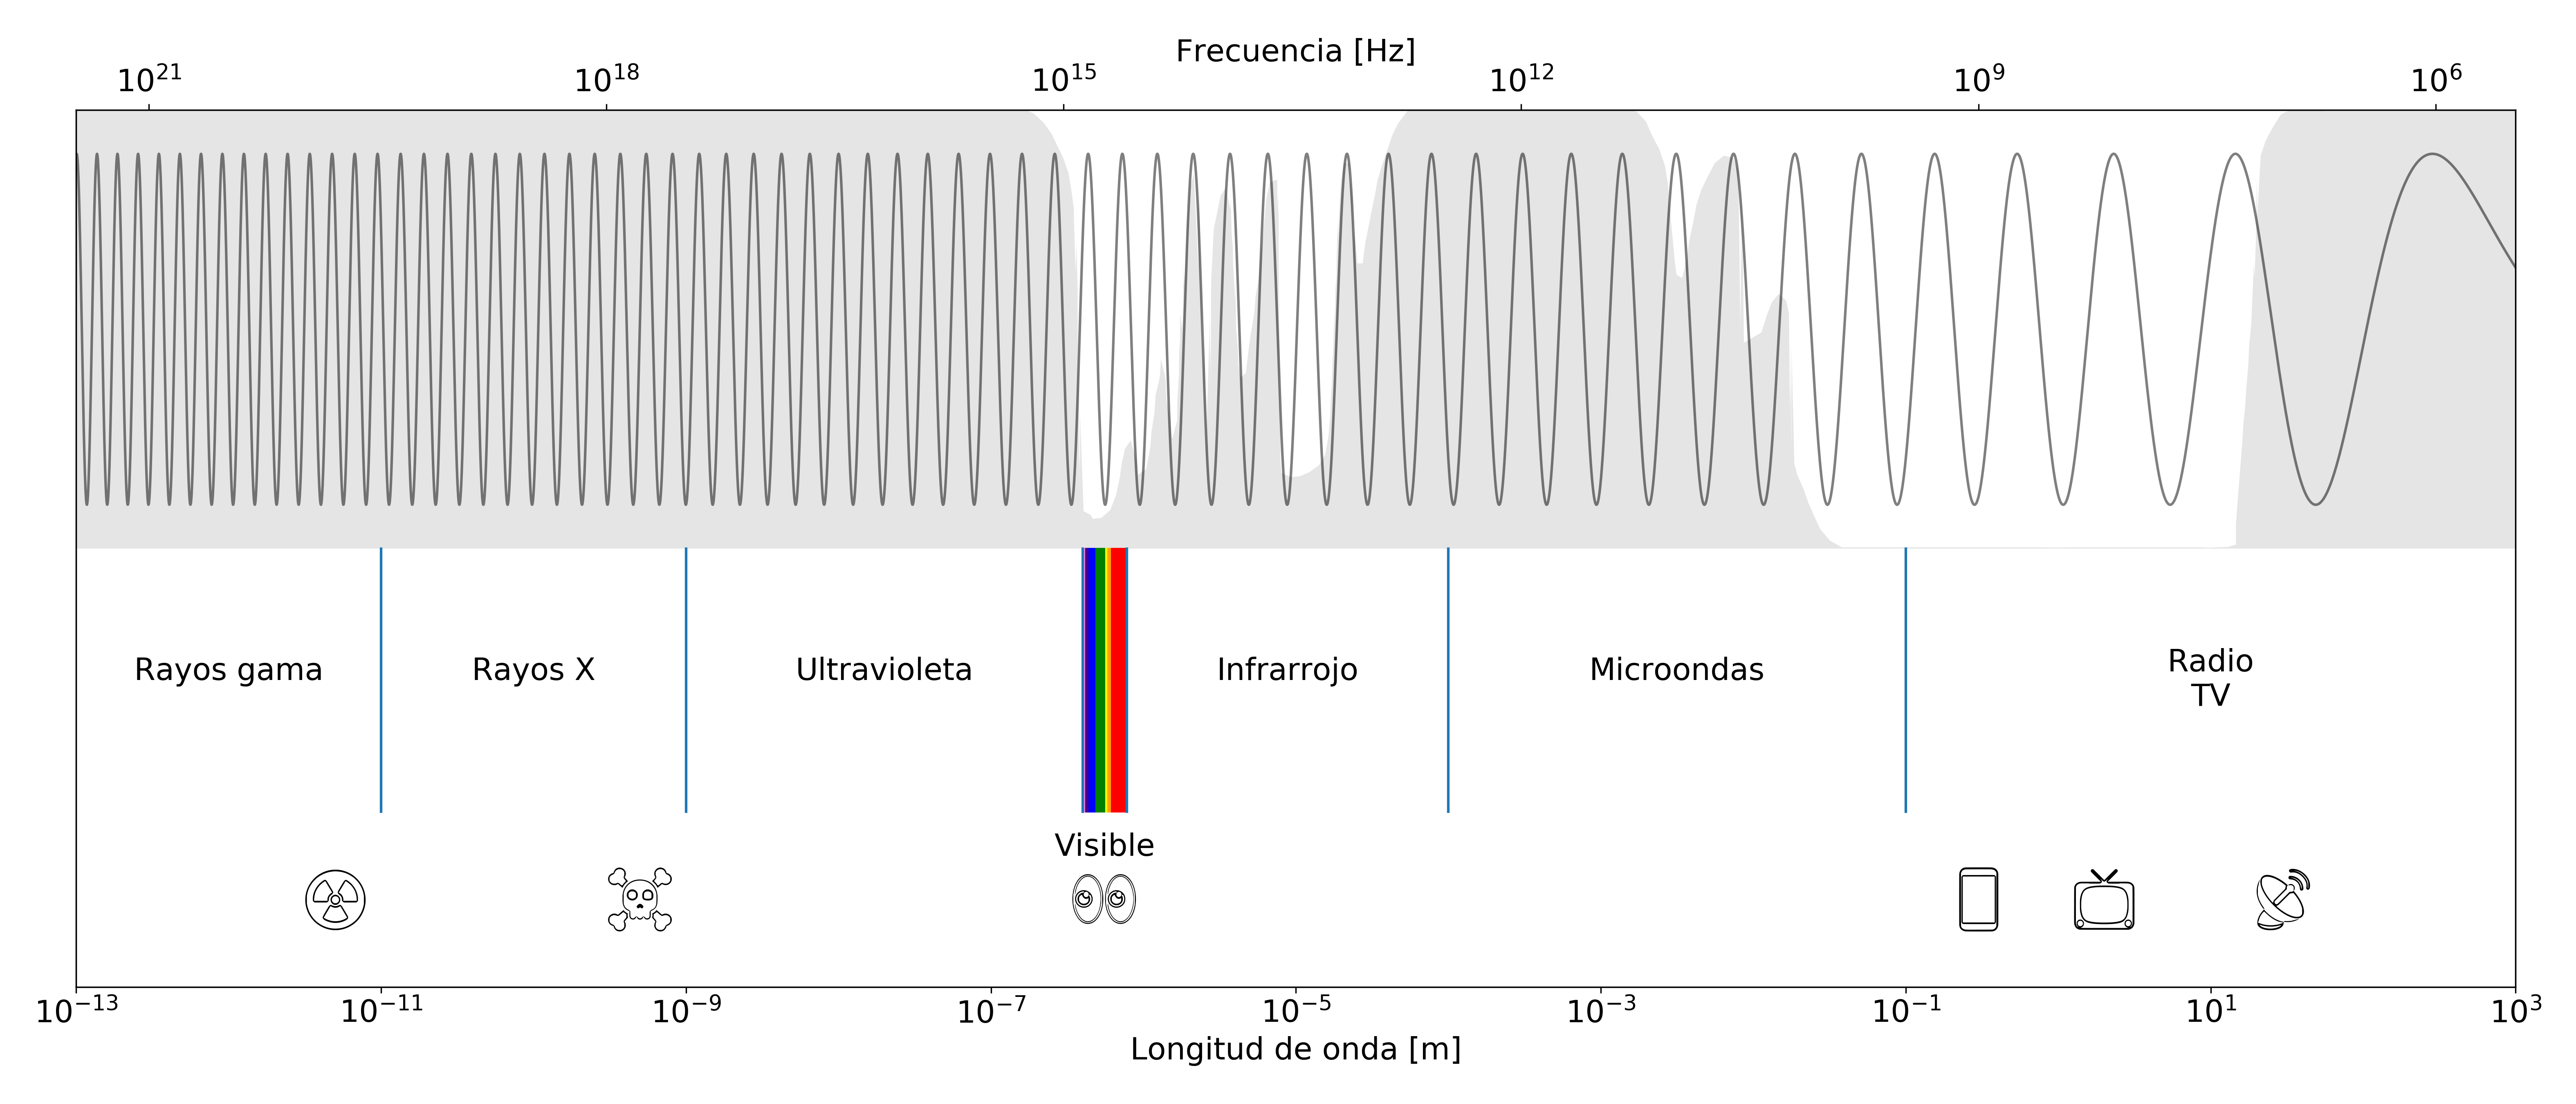
\includegraphics[width=\textwidth]{fig:espectro-pres.png}
    \caption{Espectro electromagnético en longitud de onda (abajo) y frecuencia (arriba).}
    \label{}
  \end{figure}
\end{frame}
%--- Next Frame ---%

\subsection{Funcionamiento de un radar}
\begin{frame}{} \vskip0cm
    \begin{figure}
      \centering
      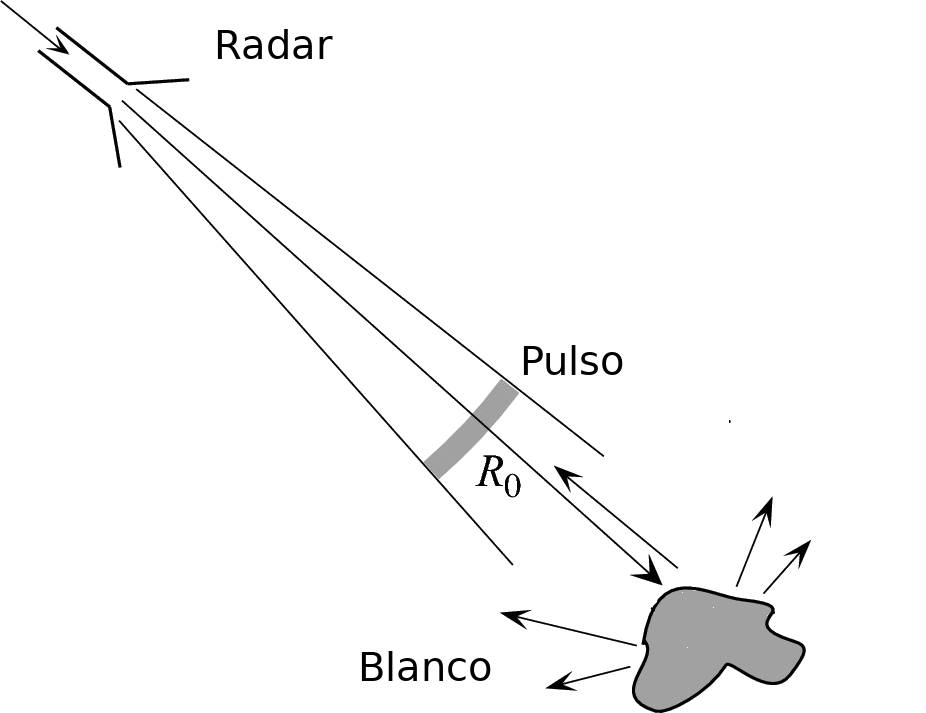
\includegraphics[scale=0.7]{fig:radar.png}
      \caption{RAdio Detection And Ranging. Funcionamiento esquemático.}
      \label{}
    \end{figure}
\end{frame}
%--- Next Frame ---%

\begin{frame}{} \vskip0cm
  \begin{figure}
    \centering
    \movie[width = \textwidth,loop,autostart]{\centering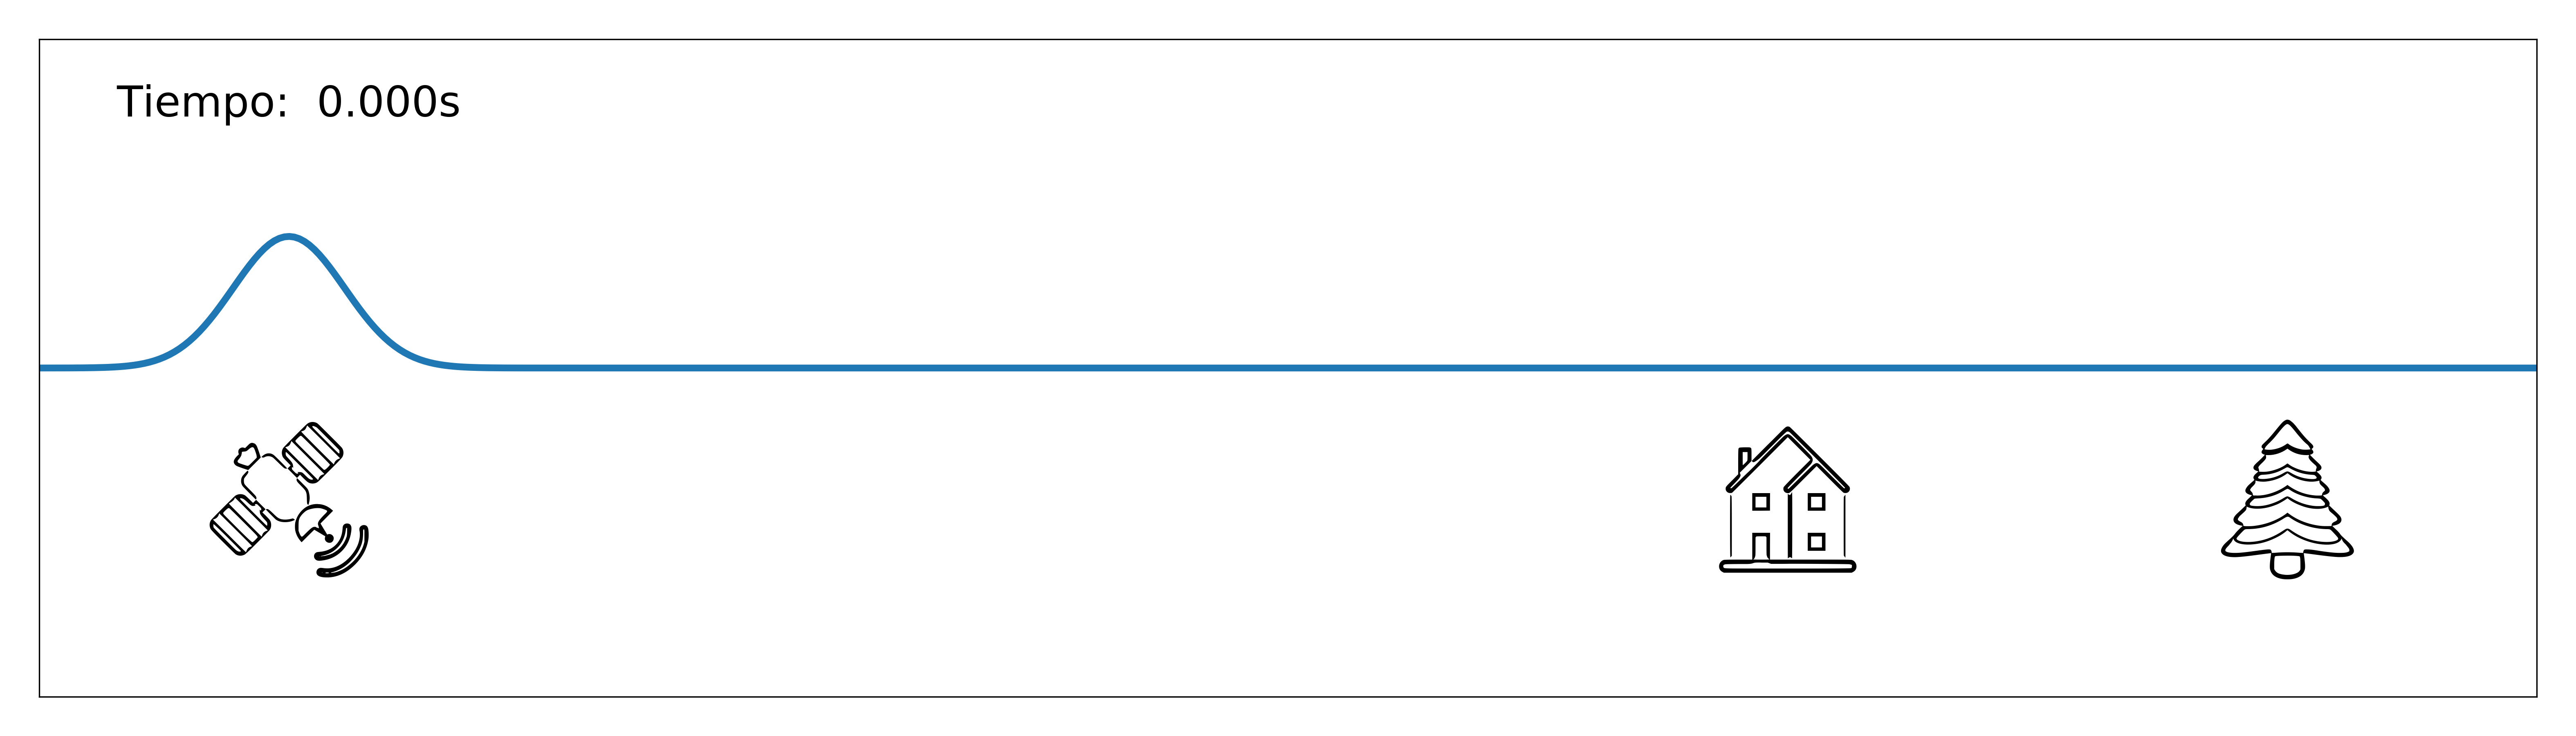
\includegraphics[width=\textwidth]{fig:funcionamiento.png}}{../figs/fig:funcionamiento.mp4}
    \caption{Ecos detectados por un radar en función del tiempo}
    \label{}
  \end{figure}
\end{frame}
%--- Next Frame ---%

\begin{frame}{} \vskip0cm
  \begin{figure}
    \centering
    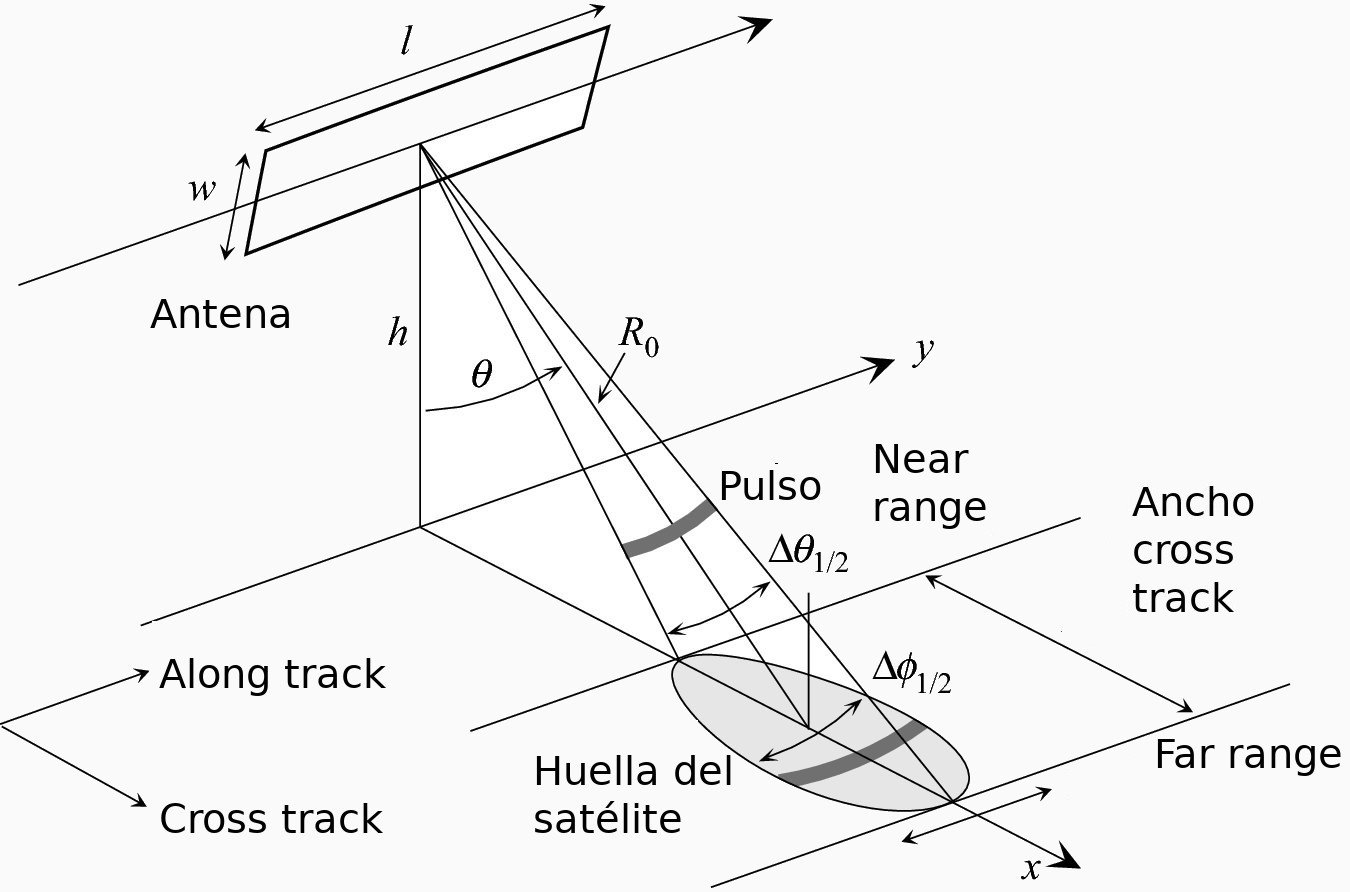
\includegraphics[scale=0.7]{01938fig13_1.jpg}
    \caption{Geometría de observación de un radar completa en la direcciones perpendiculares y paralelas al movimiento (accross track y along track)}
    \label{}
  \end{figure}
\end{frame}
%--- Next Frame ---%


\begin{frame}{} \vskip0cm
  \begin{figure}
    \centering
    \movie[width = 0.95\textwidth,loop,autostart]{\centering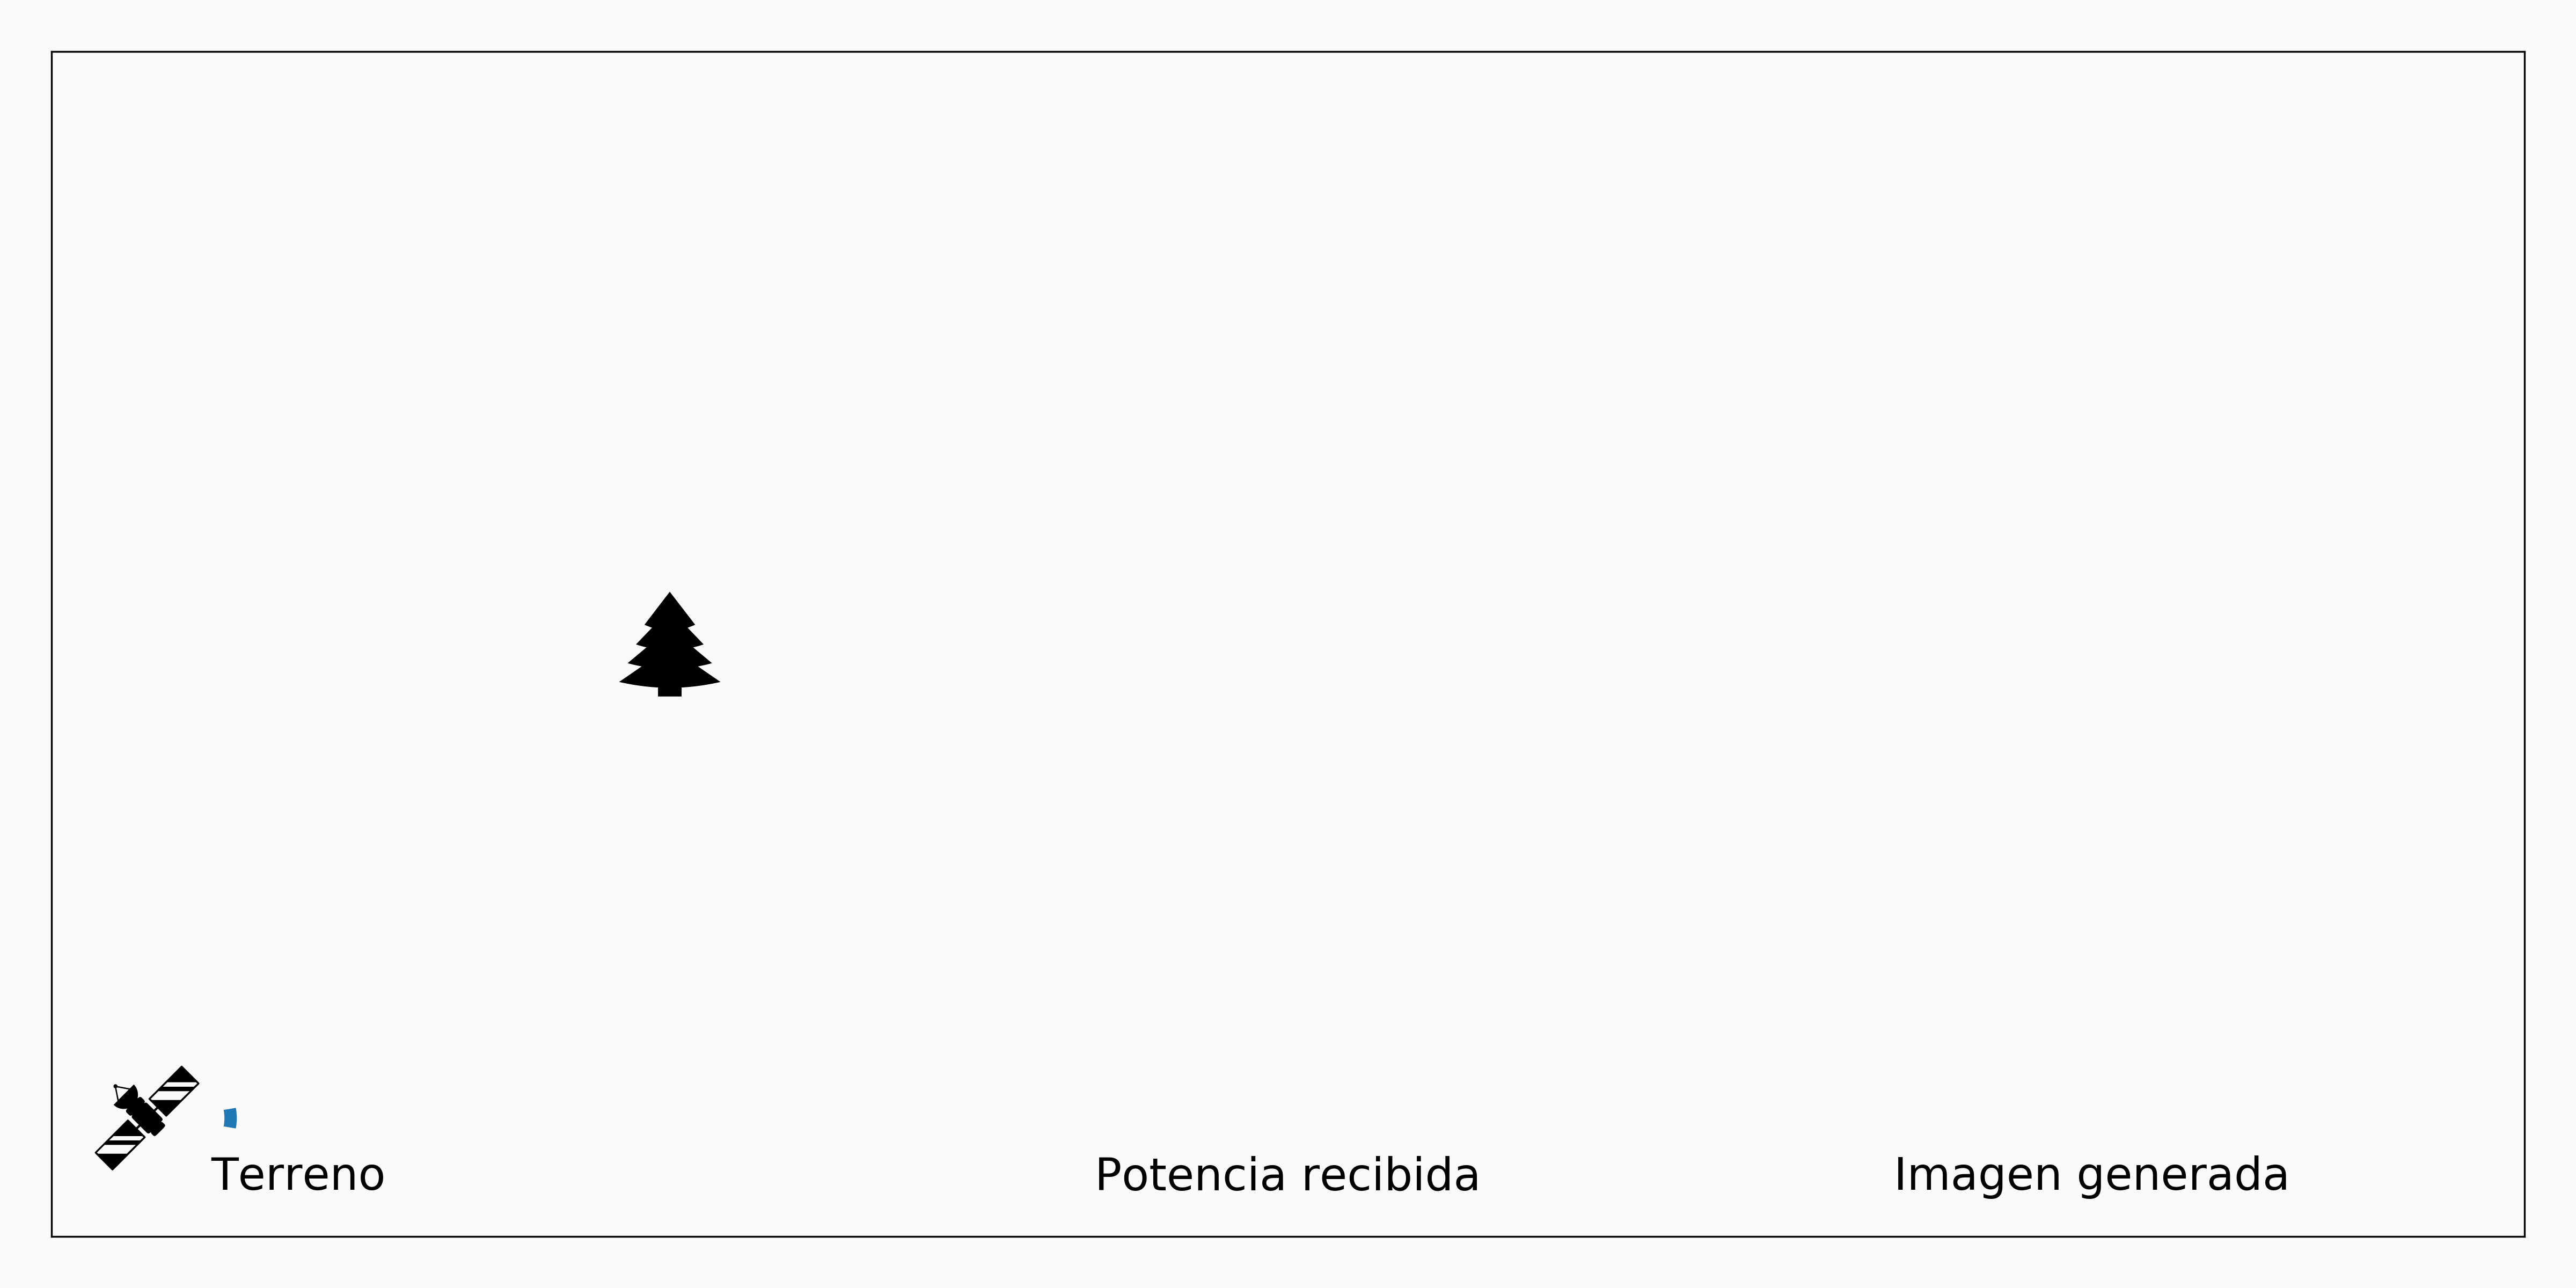
\includegraphics[width=0.95\textwidth]{fig:imagen.png}}{../figs/fig:imagen.mp4}
    \caption{Generación de una imagen radar a partir de datos en el terreno.}
    \label{}
  \end{figure}
\end{frame}
%--- Next Frame ---%

\subsection{Modos de adquisición}

\begin{frame}{} \vskip0cm
  \begin{columns}
    \begin{column}{0.5\textwidth}
       \begin{figure}
         \centering
         \movie[width = 0.95\textwidth,loop,autostart]{\centering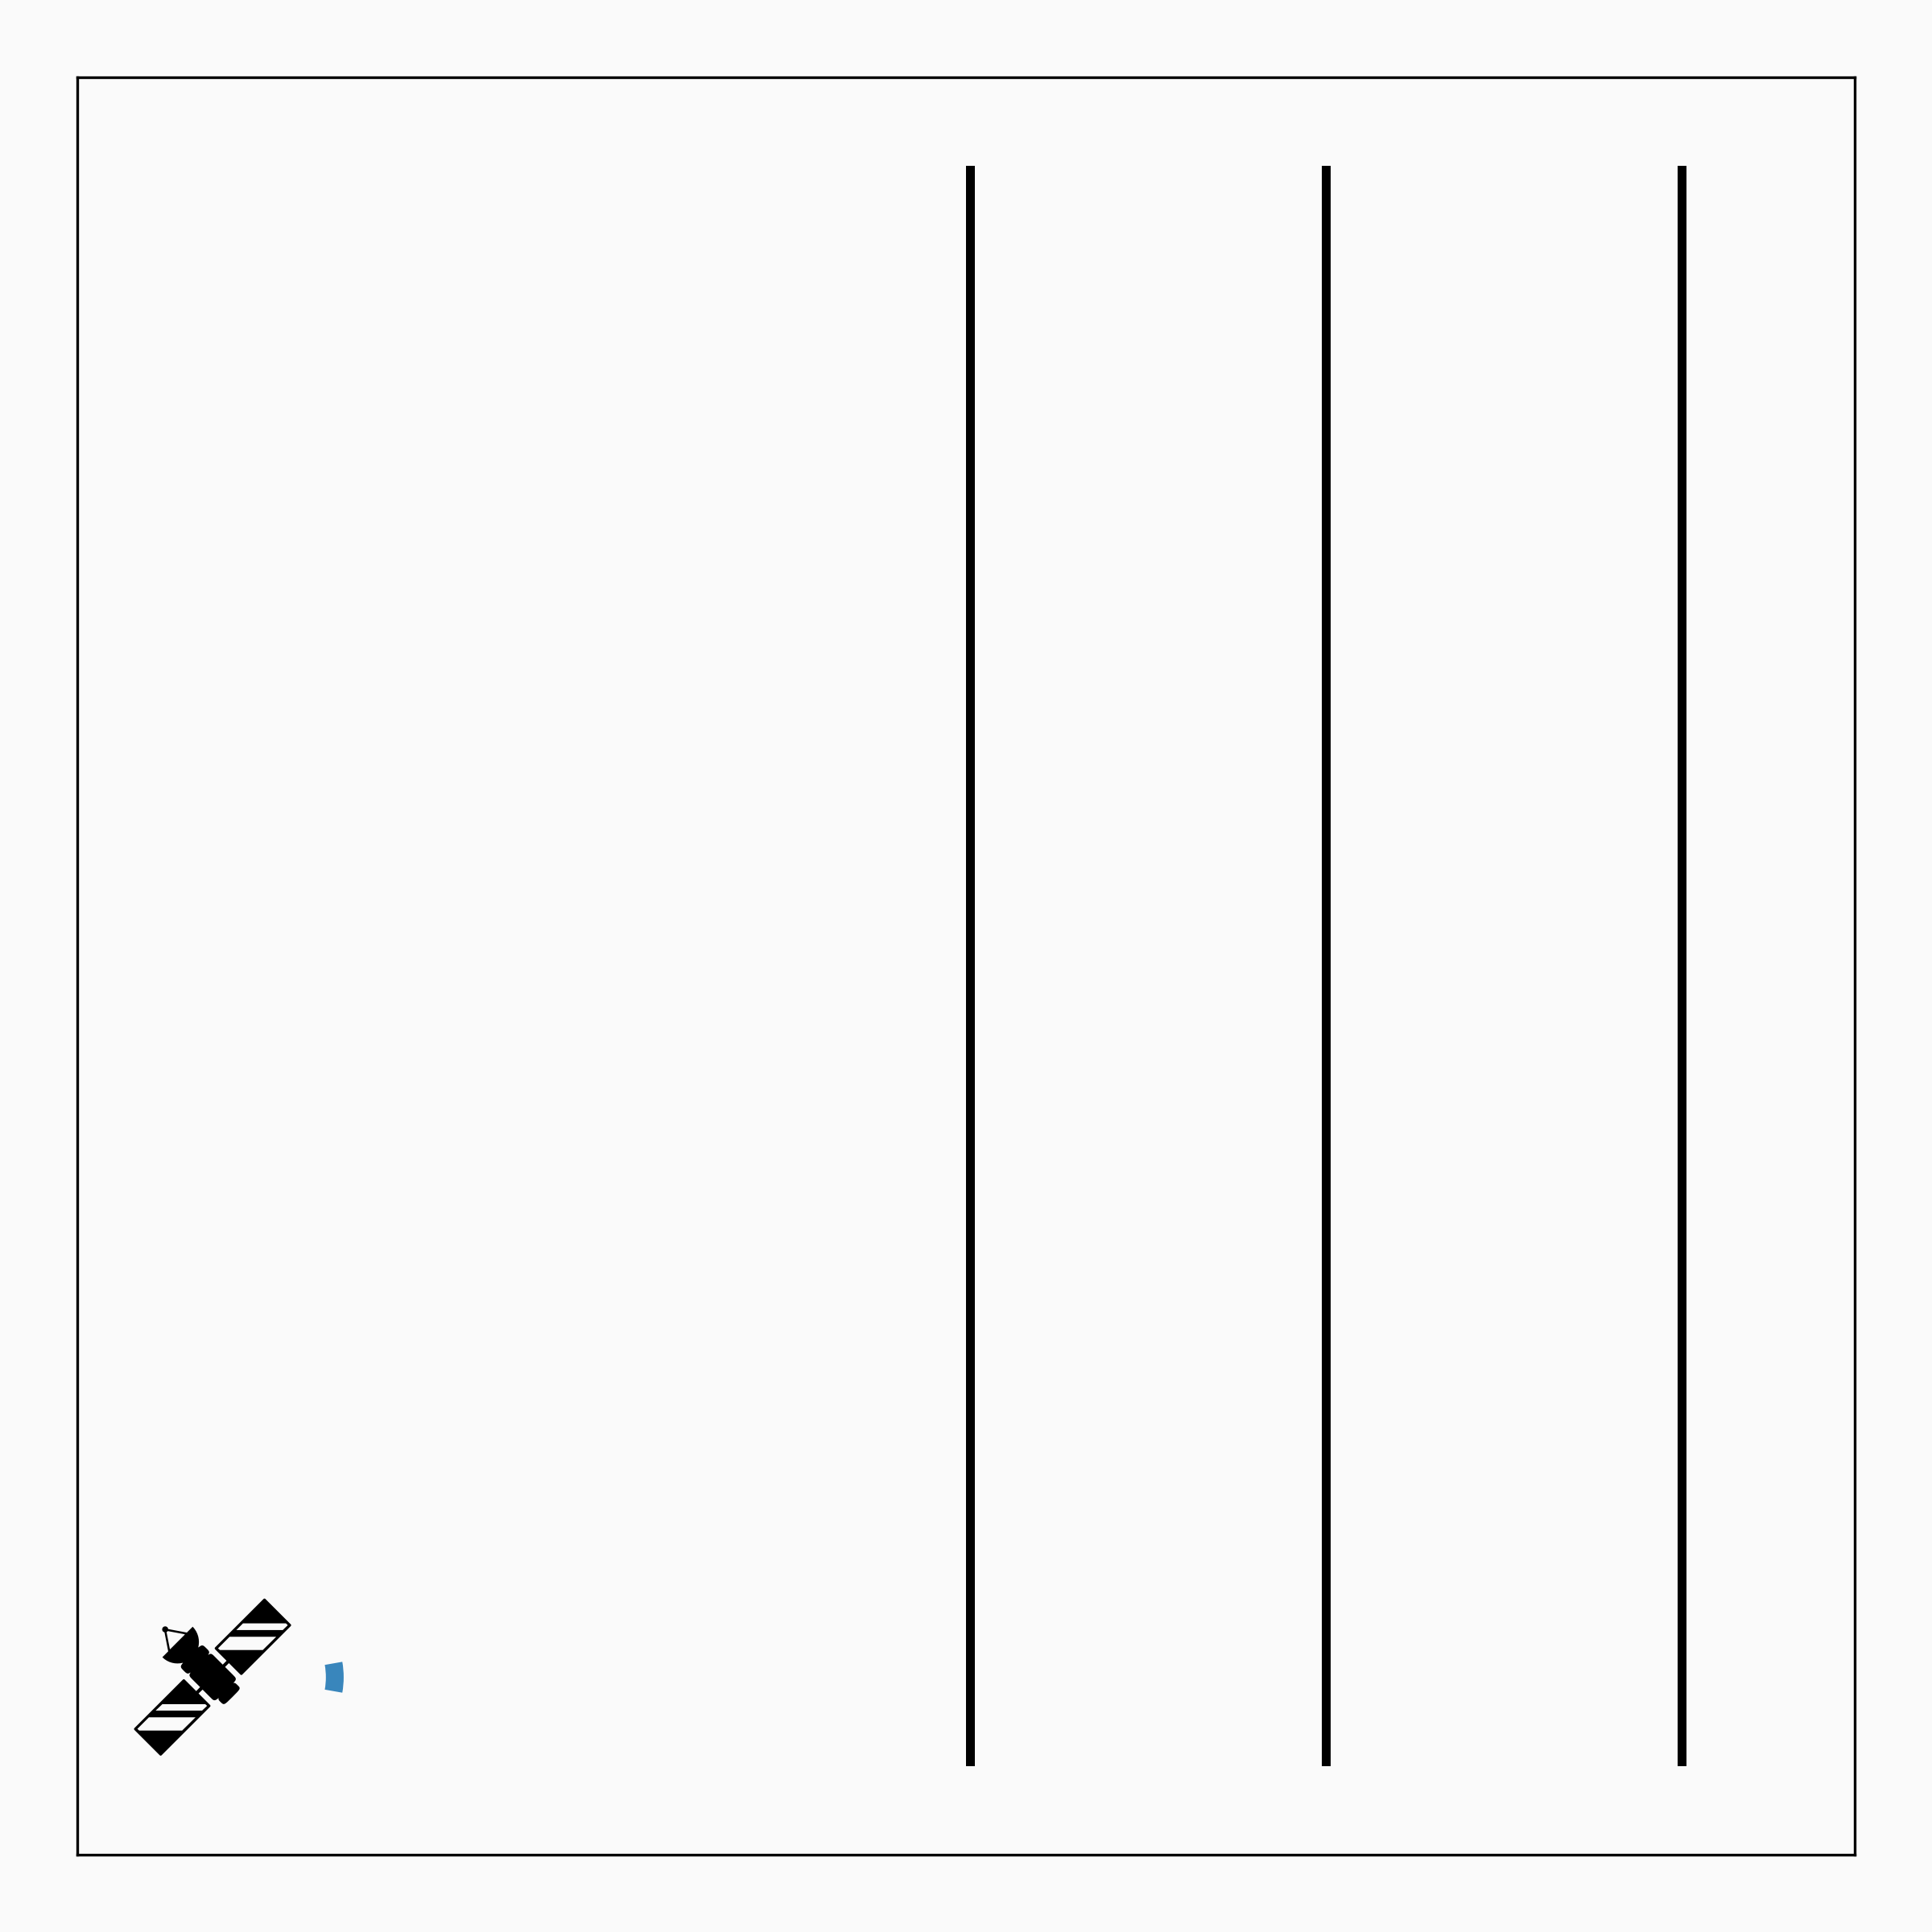
\includegraphics[width=0.95\textwidth]{fig:strip.png}}{../figs/fig:strip.mp4}
         %\caption{Modo de adquisición STRIPMAP.}
         \label{}
       \end{figure}
    \end{column}
    \begin{column}{0.5\textwidth}  %%<--- here
      \begin{block}{Modo de adquisición STRIPMAP}
        \begin{itemize}
          \item El RADAR toma datos de un solo Swadth
          \item Es el método de más básico de adquisición.
          \item Resolución espacial intermedia.
          \item Cobertura limitada.
        \end{itemize}
      \end{block}
    \end{column}
    \end{columns}
\end{frame}
%--- Next Frame ---%

\begin{frame}{} \vskip0cm
  \begin{columns}
    \begin{column}{0.5\textwidth}
       \begin{figure}
         \centering
         \movie[width = 0.95\textwidth,loop,autostart]{\centering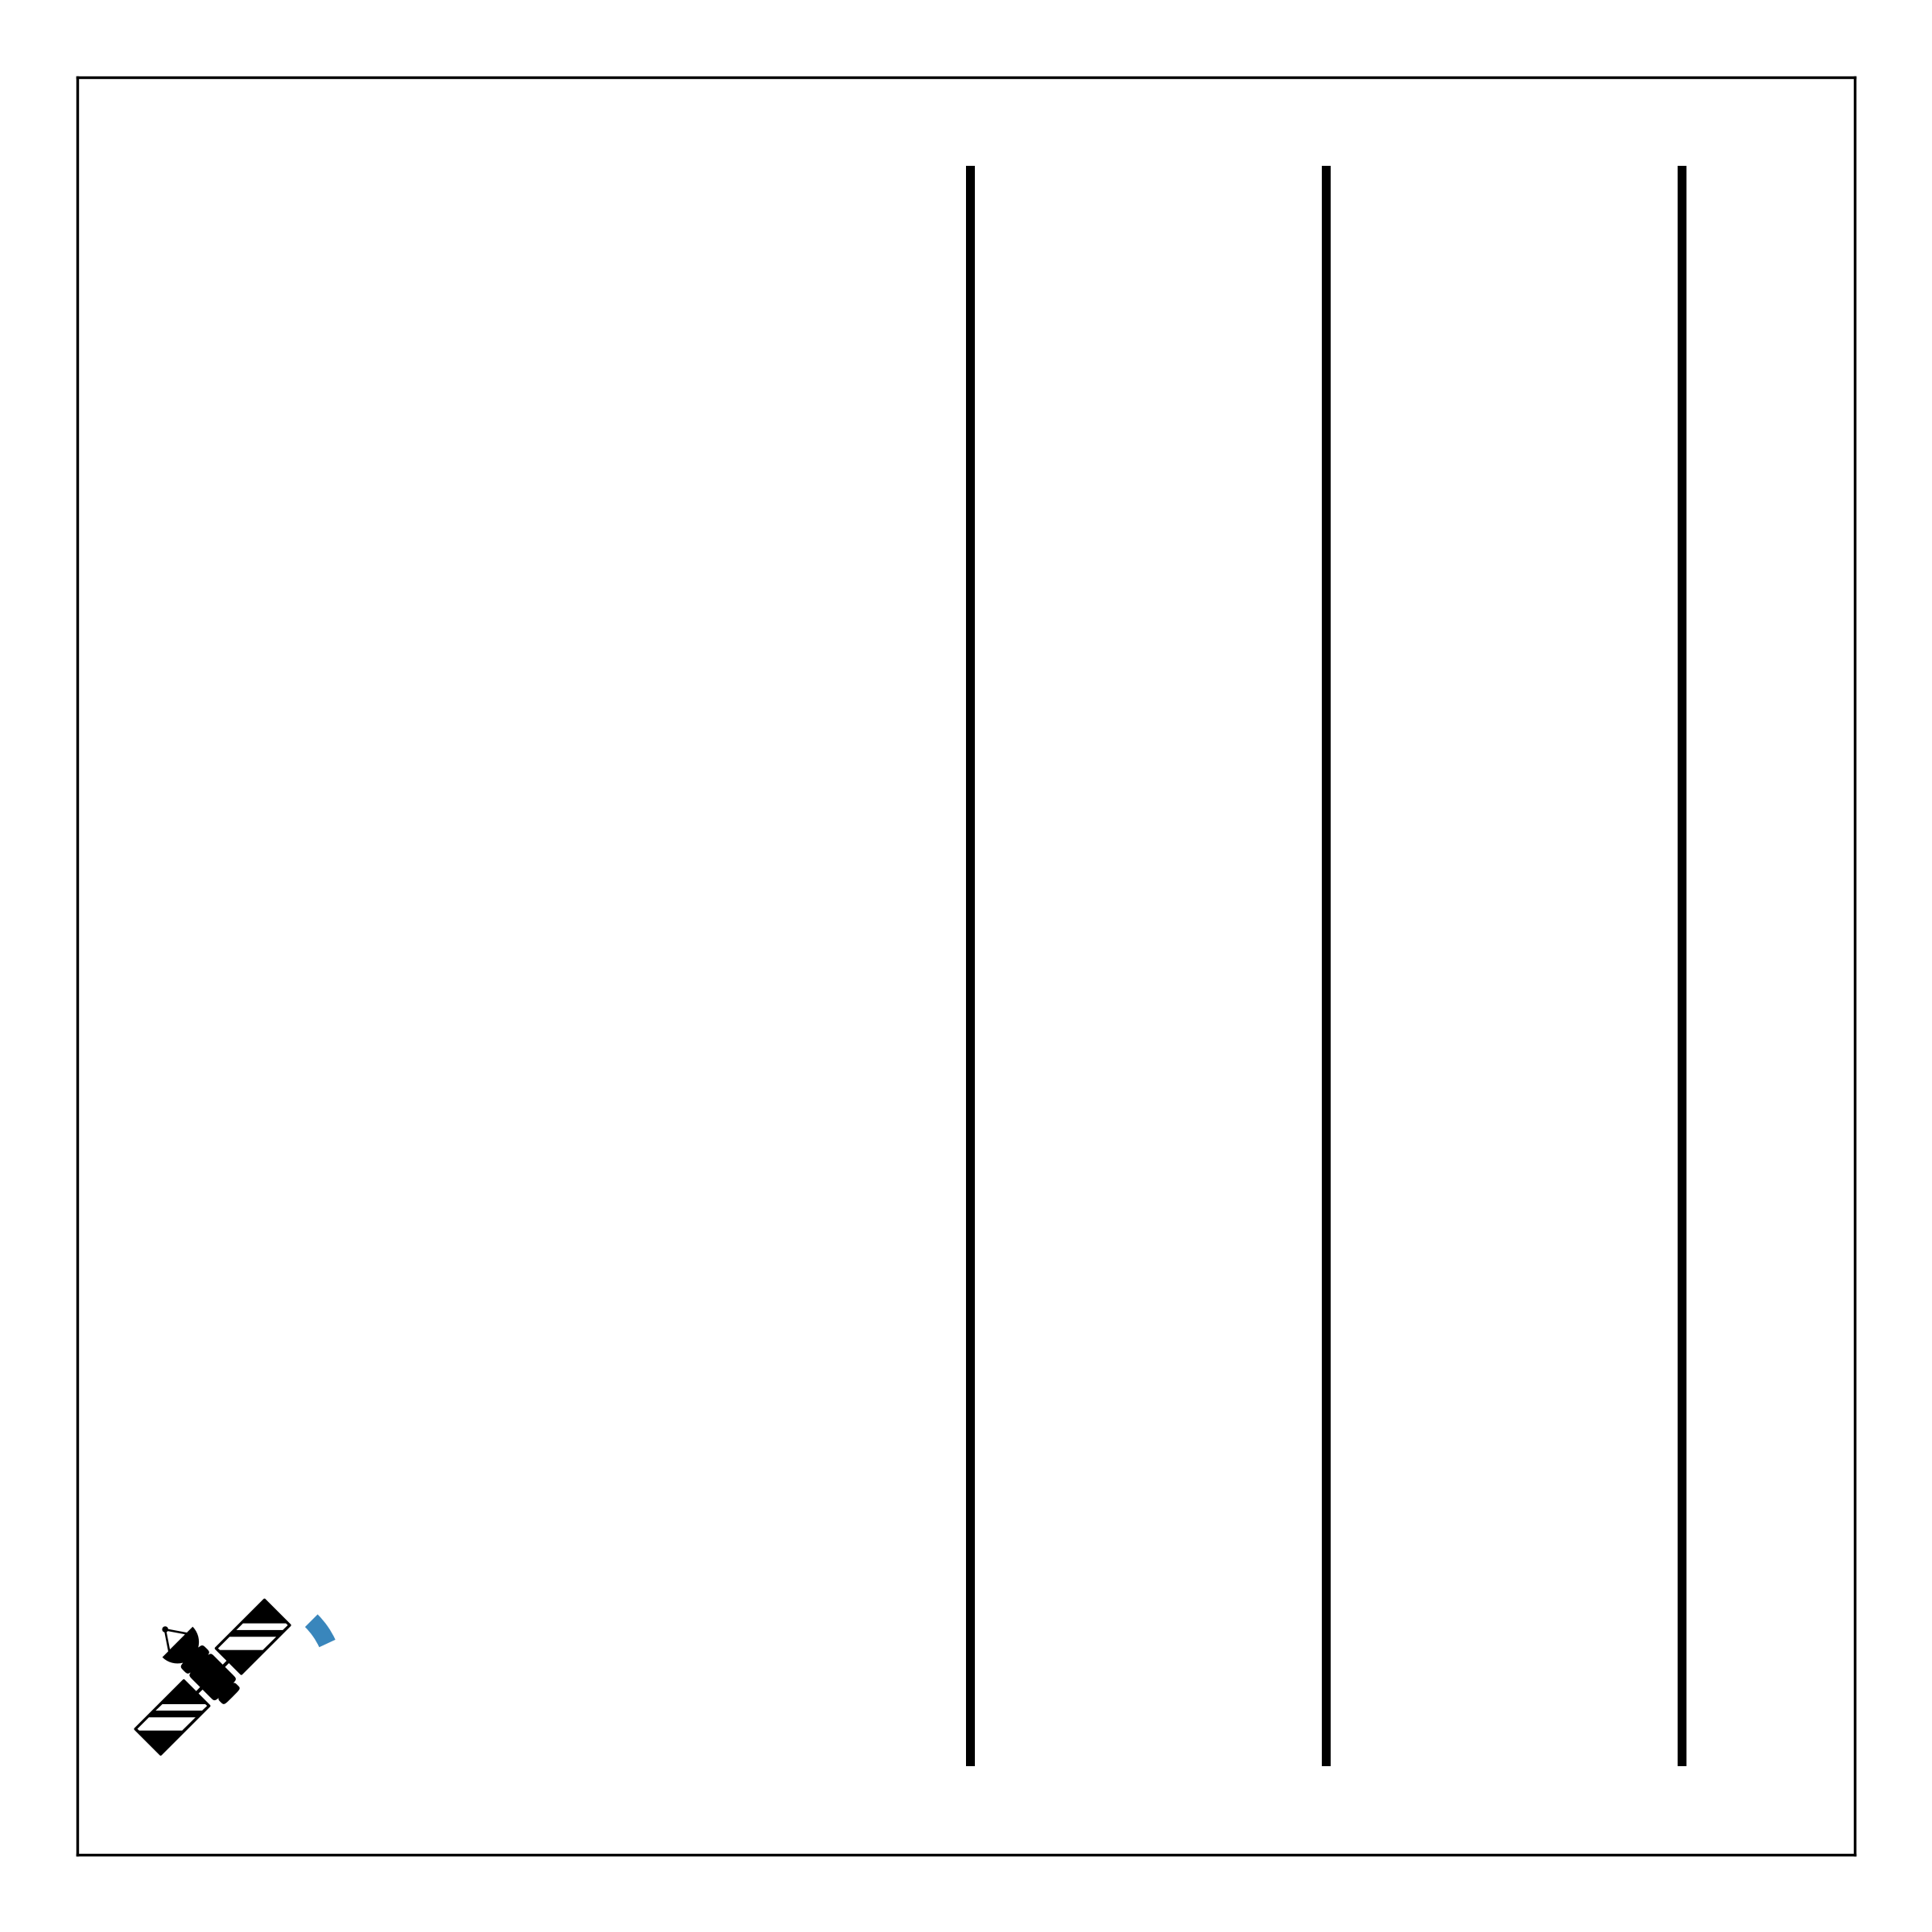
\includegraphics[width=0.95\textwidth]{fig:spot.png}}{../figs/fig:spot.mp4}
         %\caption{Modo de adquisición STRIPMAP.}
         \label{}
       \end{figure}
    \end{column}
    \begin{column}{0.5\textwidth}  %%<--- here
      \begin{block}{Modo de adquisición SPOTLIGHT}
        \begin{itemize}
          \item El RADAR observa un único blanco durante toda la pasada.
          \item Alta resolución espacial.
          \item Baja cobertura.
          \item Necesita reorientar la antena dentro de la adquisición.
        \end{itemize}
      \end{block}
    \end{column}
    \end{columns}
\end{frame}
%--- Next Frame ---%

\begin{frame}{} \vskip0cm
  \begin{columns}
    \begin{column}{0.5\textwidth}
       \begin{figure}
         \centering
         \movie[width = 0.95\textwidth,loop,autostart]{\centering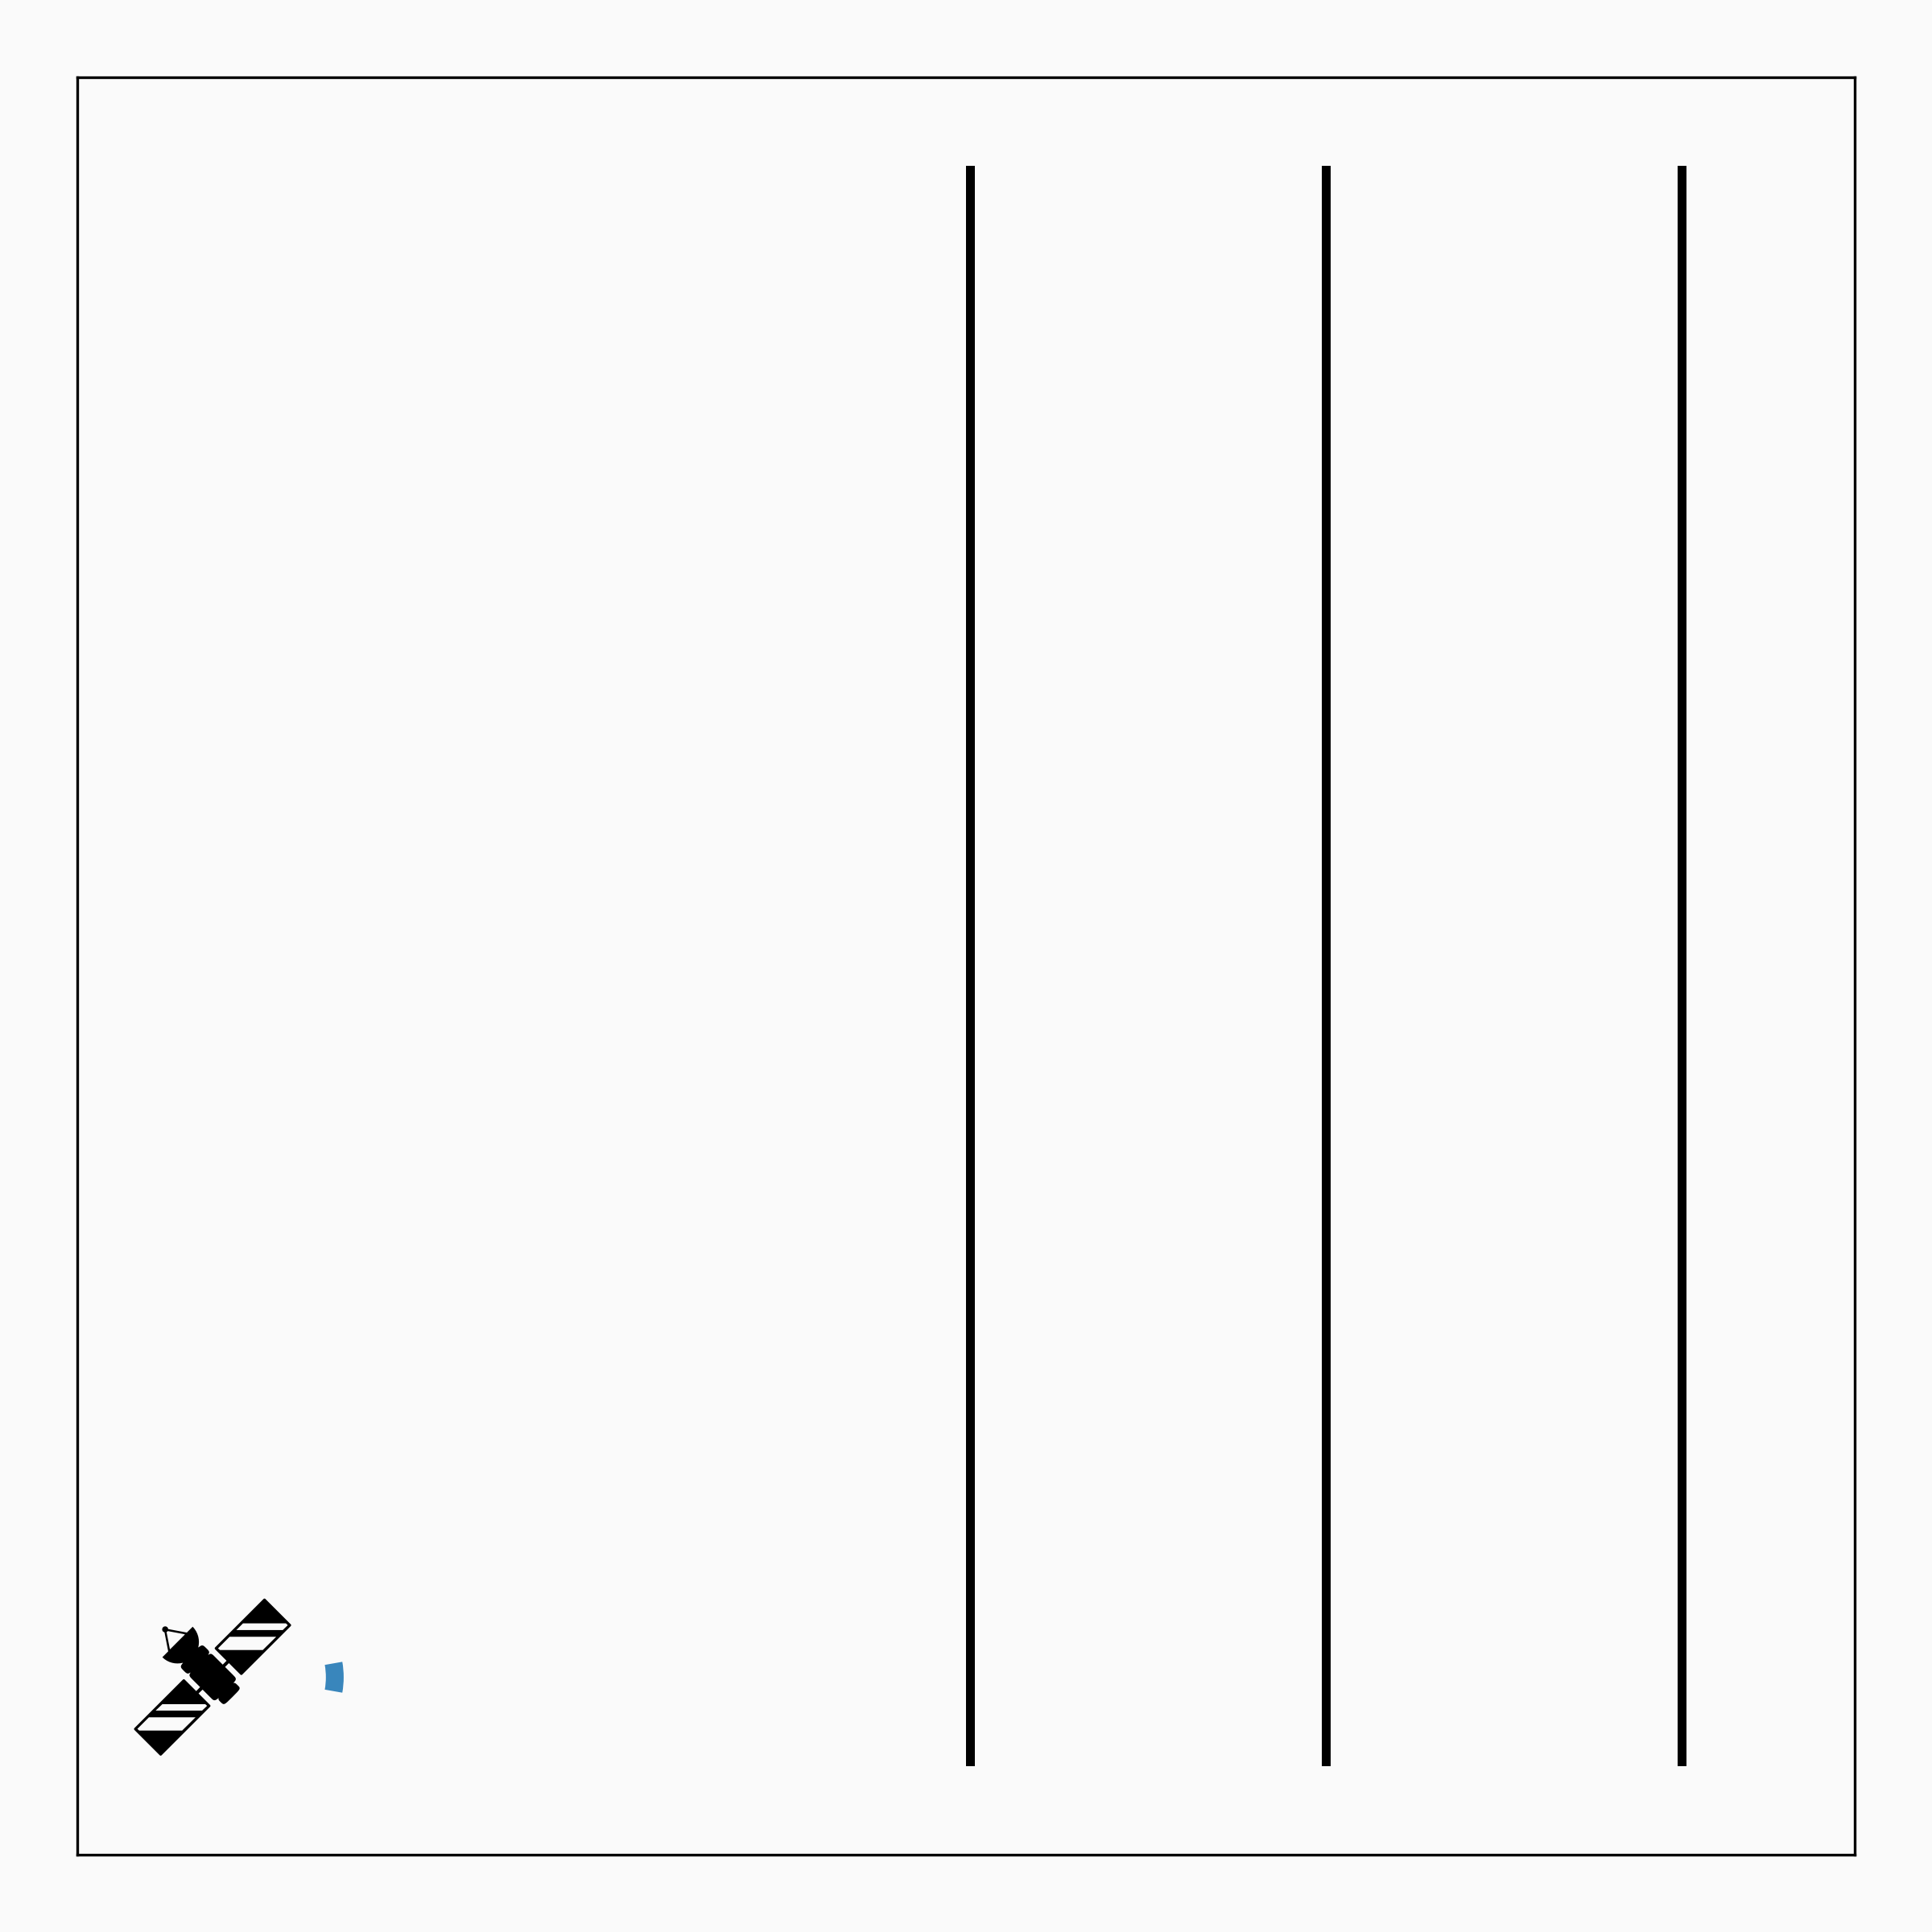
\includegraphics[width=0.95\textwidth]{fig:scan.png}}{../figs/fig:scan.mp4}
         %\caption{Modo de adquisición STRIPMAP.}
         \label{}
       \end{figure}
    \end{column}
    \begin{column}{0.5\textwidth}  %%<--- here
      \begin{block}{Modo de adquisición SCANSAR}
        \begin{itemize}
          \item El RADAR Va distribuyendo pulsos de a bursts entre varios swaths.
          \item Baja resolución.
          \item Gran cobertura.
          \item Mala distribución espacial de potencia.
          \item Hace falta reapuntar la antena en elevación entre burst.
        \end{itemize}
      \end{block}
    \end{column}
    \end{columns}
\end{frame}
%--- Next Frame ---%
\begin{frame}{} \vskip0cm
  \begin{columns}
    \begin{column}{0.5\textwidth}
       \begin{figure}
         \centering
         \movie[width = 0.95\textwidth,loop,autostart]{\centering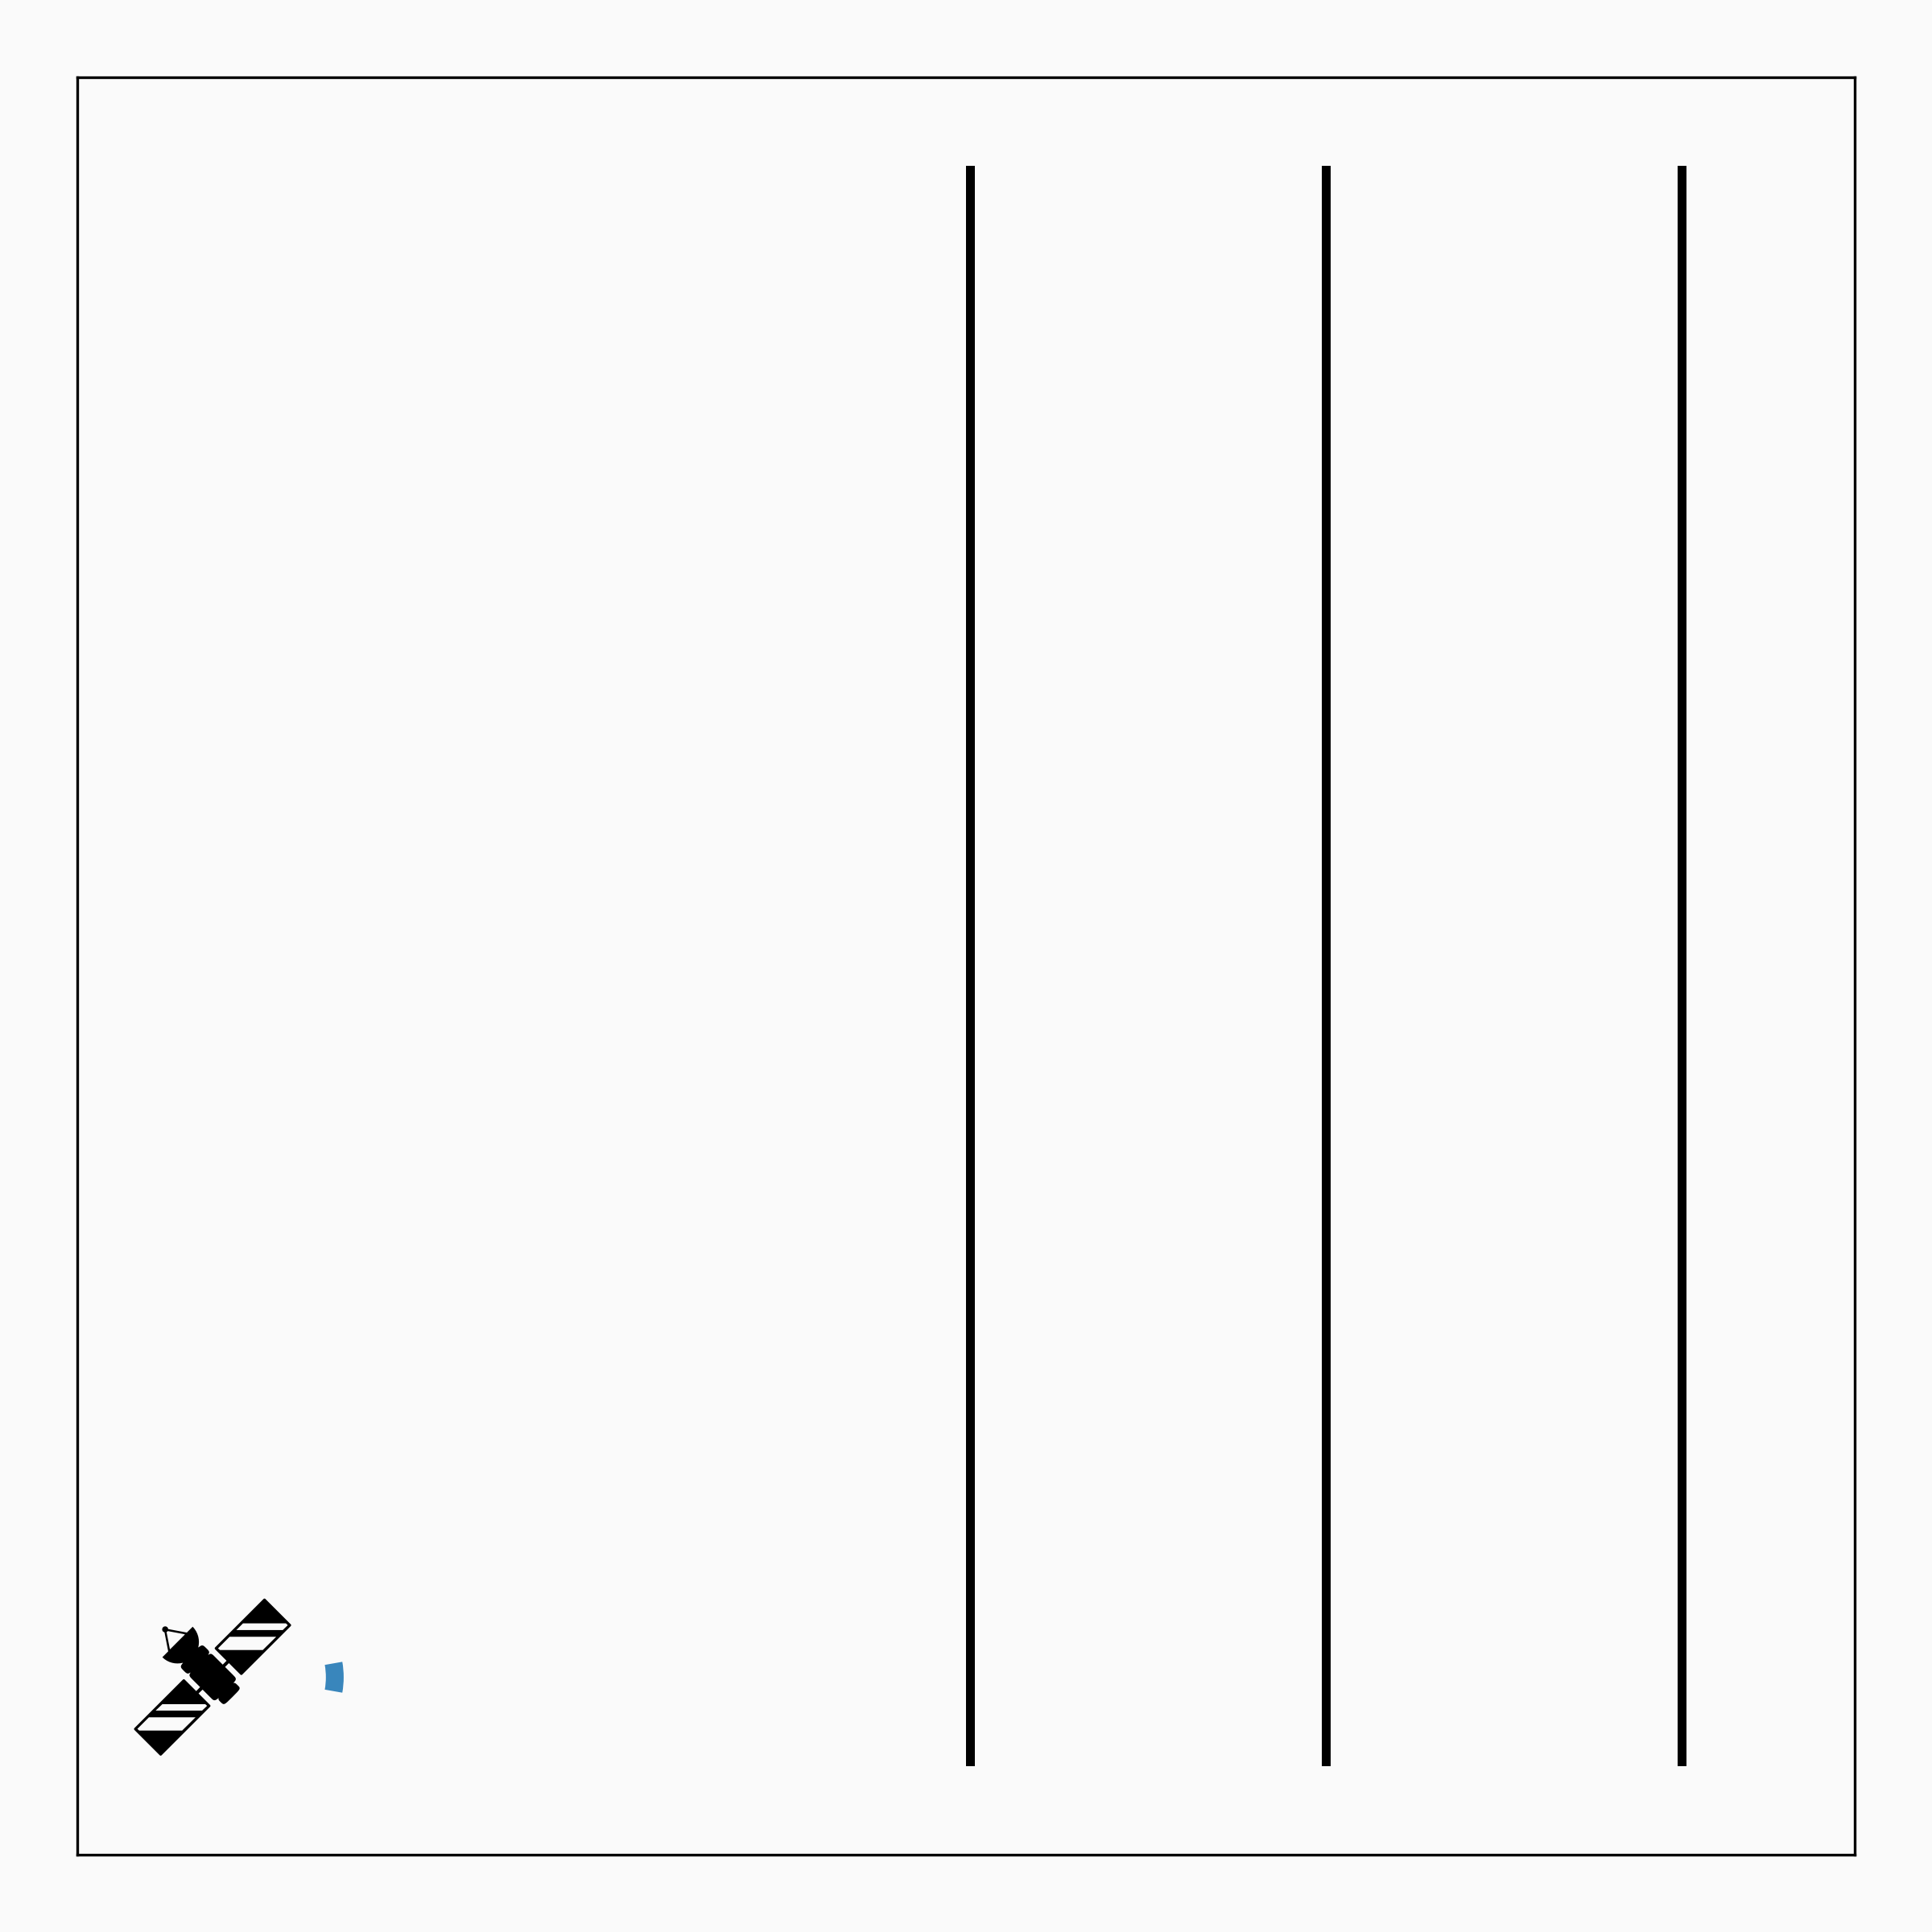
\includegraphics[width=0.95\textwidth]{fig:top.png}}{../figs/fig:top.mp4}
         %\caption{Modo de adquisición STRIPMAP.}
         \label{}
       \end{figure}
    \end{column}
    \begin{column}{0.5\textwidth}  %%<--- here
      \begin{block}{Modo de adquisición TOPSAR}
        \begin{itemize}
          \item El RADAR Va distribuyendo pulsos entre varios swaths y variando el apuntamiento en acimut para iluminar la pisada de manera mas homogénea.
          \item Baja resolución.
          \item Gran cobertura.
          \item Buena distribución de potencia.
        \end{itemize}
      \end{block}
    \end{column}
    \end{columns}
\end{frame}
%--- Next Frame ---%

\begin{frame}{} \vskip0cm
\begin{columns}
  \begin{column}{0.5\textwidth}
   \begin{block}{Óptico}
     \begin{itemize}
       \item Rango de trabajo en los micrometros ($0.3\mu$ m a $2.5\mu m$).
       %\item Detecta luz solar reflejada por la tierra.
       \item Afectado por las condiciones atmosféricas.
       %\item Detecta luz incoherente.
       \item Depende de una fuente de iluminación externa.
     \end{itemize}
   \end{block}
  \end{column}
  \begin{column}{0.5\textwidth}  %%<--- here
    \begin{block}{Radar}
      \begin{itemize}
        \item Rango de trabajo en los microondas ($1cm$ m a $100cm$).
        %\item Emite una señal y mide la intesidad del eco.
        \item Independiente de las condiciones atmosféricas.
        %\item Emite y detecta una onda coherente.
        \item Cuenta con su propia fuente de iluminación.
      \end{itemize}
    \end{block}
  \end{column}
  \end{columns}
\end{frame}
%--- Next Frame ---%

%\gracias
%--- Next Frame ---%

\section{Interacción con el blanco}
\subsection{¿Que es una imagen SAR?}
\begin{frame}{} \vskip0cm
  \begin{columns}[t]
    \begin{column}{0.5\textwidth}
     \begin{block}{SAR}
       \begin{itemize}
         \item Una imagen SAR es un mapa de reflectividad.
         \item Indica cuanta energía vuelve al sensor.
         \item La cantidad de energía retrodispersada depende de la geometría del blanco y su conductividad eléctrica.
         \item Las zonas oscuras y brillantes son zonas de baja y alta reflectividad.
       \end{itemize}
     \end{block}
    \end{column}
    \begin{column}{0.5\textwidth}  %%<--- here
        \begin{figure}
          \centering
          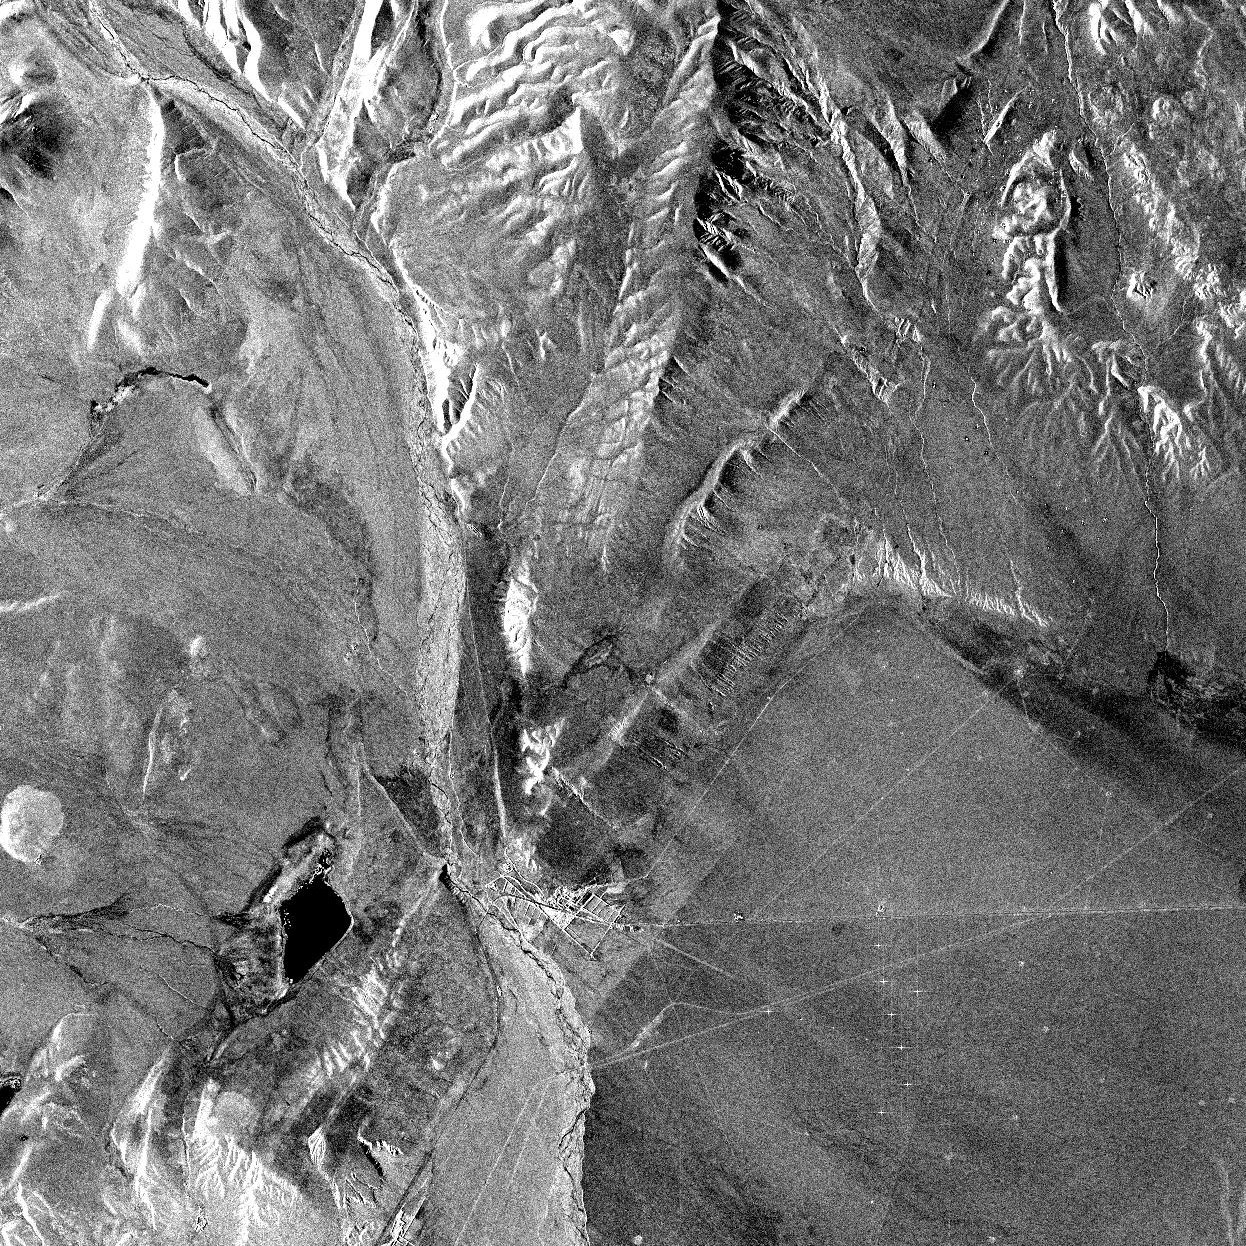
\includegraphics[width=0.8\textwidth]{fig:sar.jpg}
          \caption{Imagen SAR de una zona montañosa.}
          \label{}
        \end{figure}
    \end{column}
    \end{columns}
\end{frame}
%--- Next Frame ---%

\begin{frame}{} \vskip0cm
    \begin{figure}
      \centering
      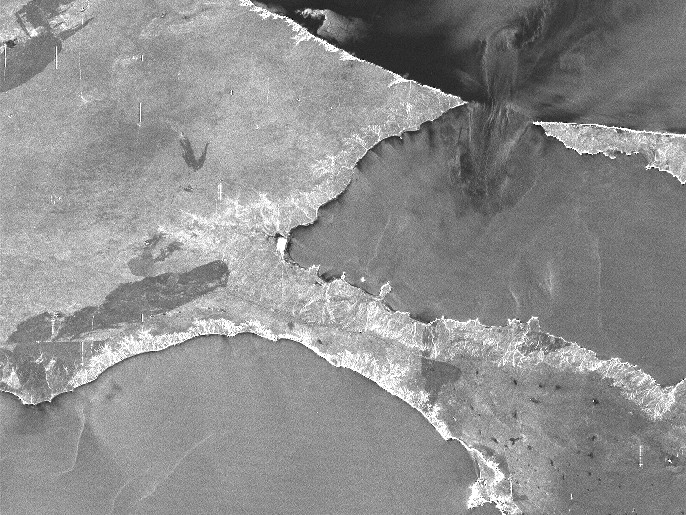
\includegraphics[width=0.6\textwidth]{fig:sar2.jpg}
      \caption{Imagen SAR de una región costera.}
      \label{}
    \end{figure}
\end{frame}
%--- Next Frame ---%

\subsection{Mecanismos de scattering}

\begin{frame}{} \vskip0cm
    \begin{figure}
      \centering
      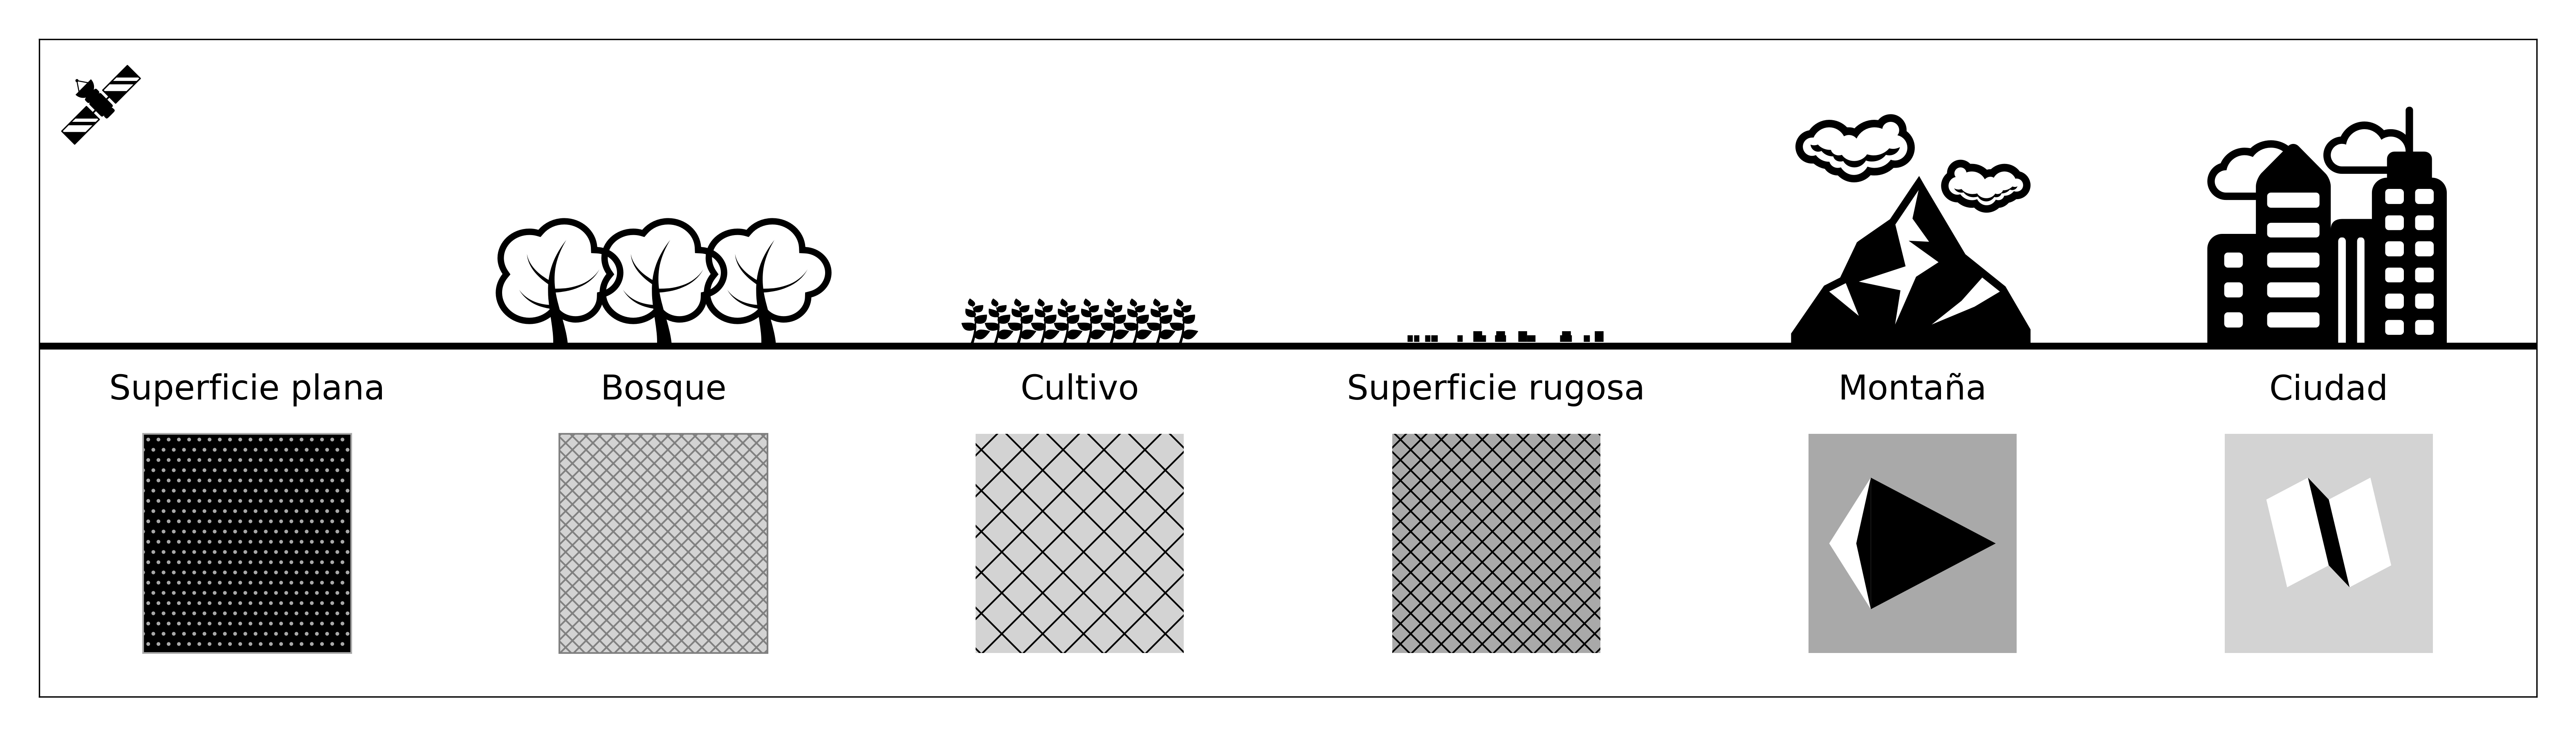
\includegraphics[width=\textwidth]{fig:blancos.png}
      \caption{Interpretación visual de distintos blancos en una imagen SAR considerando tono y textura. Pueden verse los mecanismos de interacción especular, en volumen y doble rebote.}
      \label{}
    \end{figure}
\end{frame}
%--- Next Frame ---%

\begin{frame}{} \vskip0cm
    \begin{figure}
      \centering
      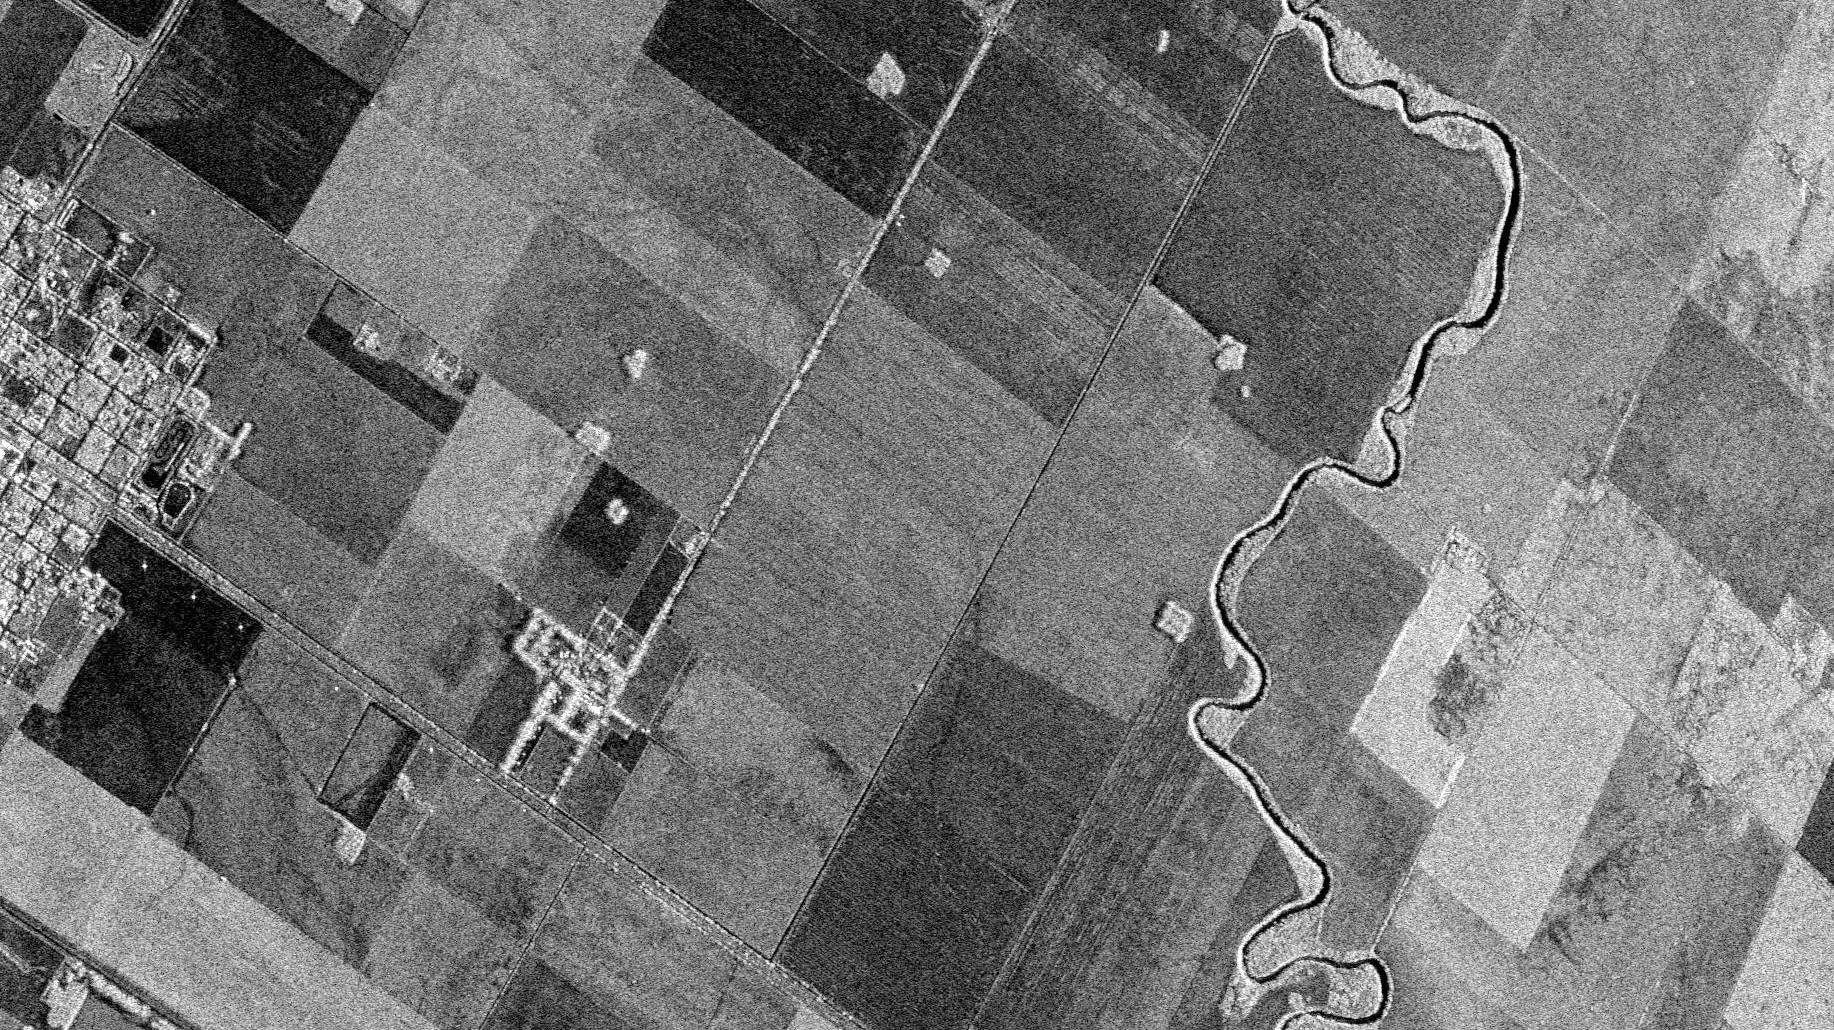
\includegraphics[width=0.6\textwidth]{fig:rebotes2.jpg}
      \caption{Imagen SAR de un área con cultivos. Pueden observarse varios de los mecanismos de interacción anteriores.}
      \label{}
    \end{figure}
\end{frame}
%--- Next Frame ---%

\begin{frame}{} \vskip0cm
  \begin{figure}
    \centering
    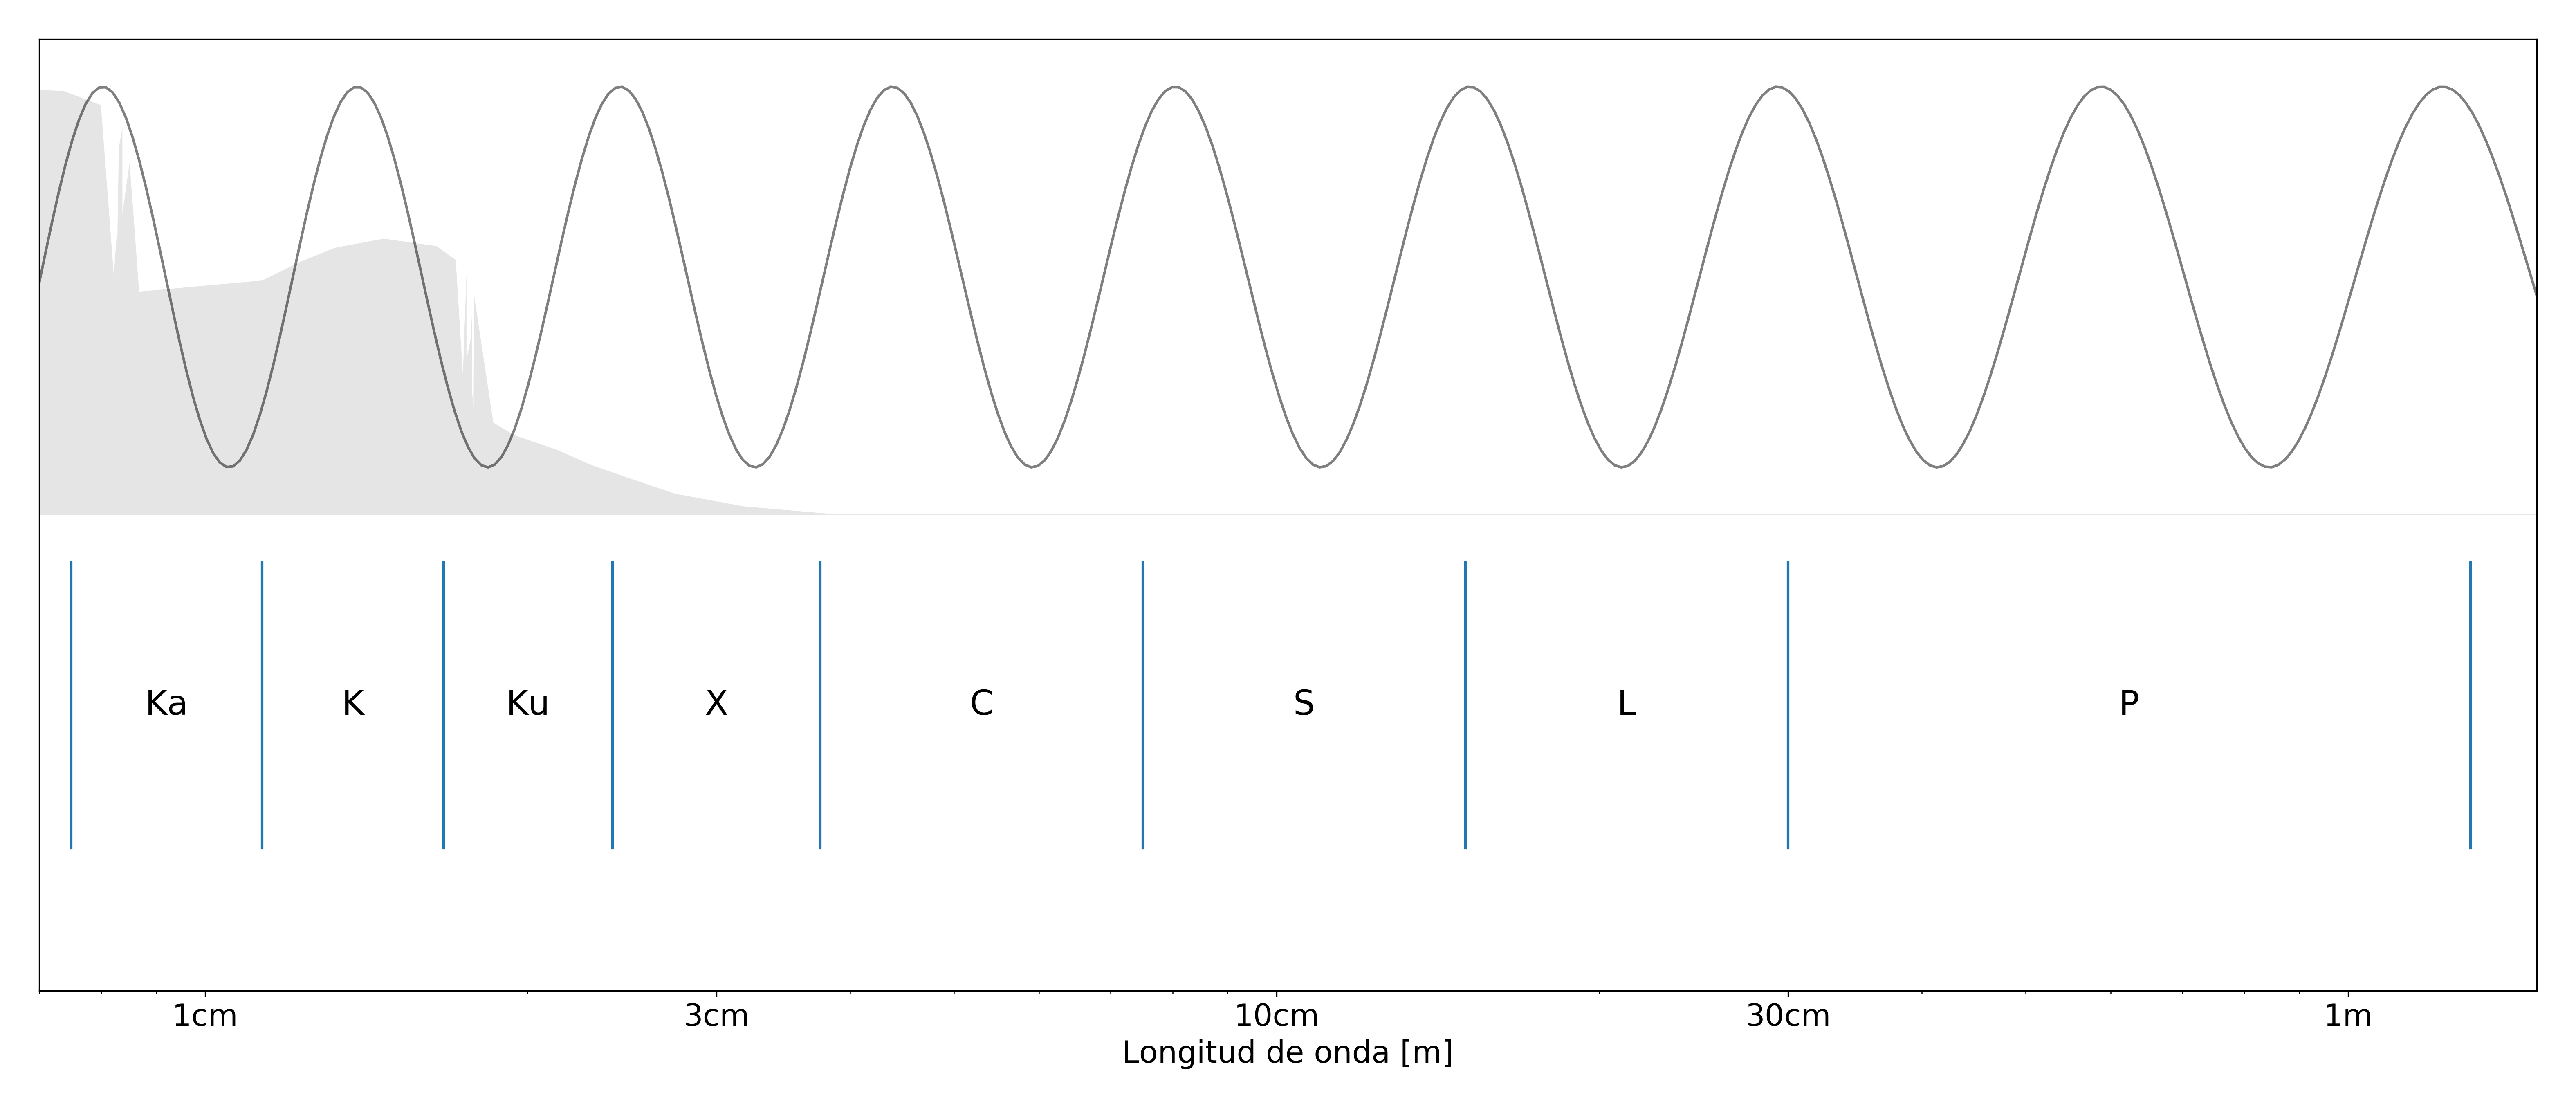
\includegraphics[width=\textwidth]{fig:espectrozoom.png}
    \caption{Espectro electromagnético en longitud de onda para la región de las microondas.}
    \label{}
  \end{figure}
\end{frame}
%--- Next Frame ---%

%\begin{frame}{} \vskip0cm
%    \begin{figure}
%      \centering
%      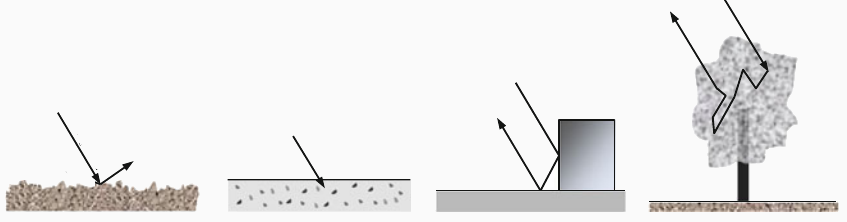
\includegraphics[width=0.9\textwidth]{fig:interacciones.png}
%      \caption{Interacciones entre los distintos blancos según la longitud de onda. De izquierda a derecha: especular, absorción, doble rebote y en volumen.}
%      \label{}
%    \end{figure}
%\end{frame}
%--- Next Frame ---%

\begin{frame}{} \vskip0cm
    \begin{figure}
      \centering
      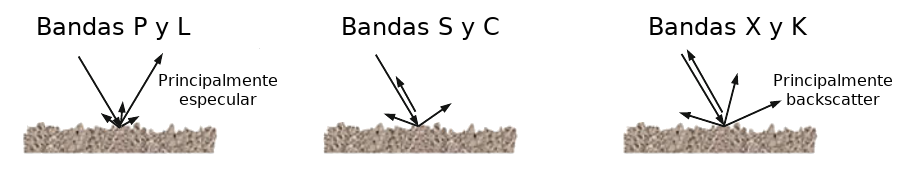
\includegraphics[width=\textwidth]{fig:interacciones-1.png}
      \caption{Interacciones entre los distintos blancos según la longitud de onda.}
      \label{}
    \end{figure}
\end{frame}
%--- Next Frame ---%

\begin{frame}{} \vskip0cm
    \begin{figure}
      \centering
      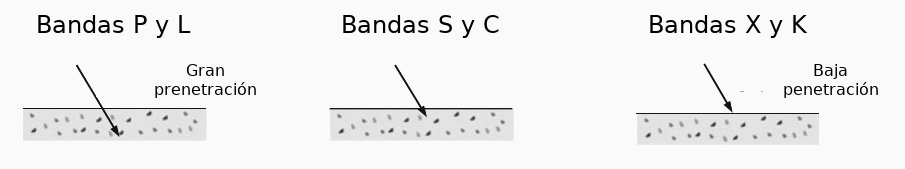
\includegraphics[width=\textwidth]{fig:interacciones-2.png}
      \caption{Interacciones entre los distintos blancos según la longitud de onda.}
      \label{}
    \end{figure}
\end{frame}
%--- Next Frame ---%

\begin{frame}{} \vskip0cm
    \begin{figure}
      \centering
      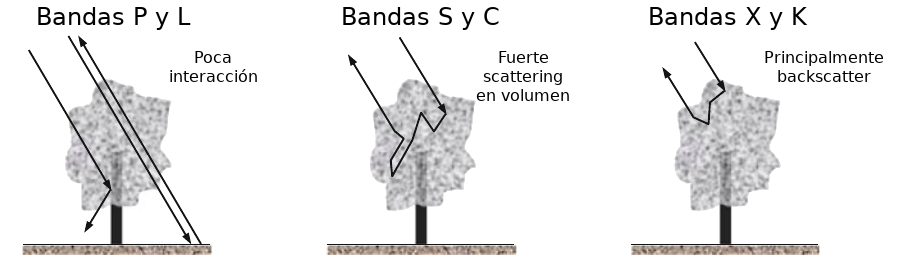
\includegraphics[width=\textwidth]{fig:interacciones-4.png}
      \caption{Interacciones entre los distintos blancos según la longitud de onda.}
      \label{}
    \end{figure}
\end{frame}
%--- Next Frame ---%

\begin{frame}{} \vskip0cm
    \begin{figure}
      \centering
      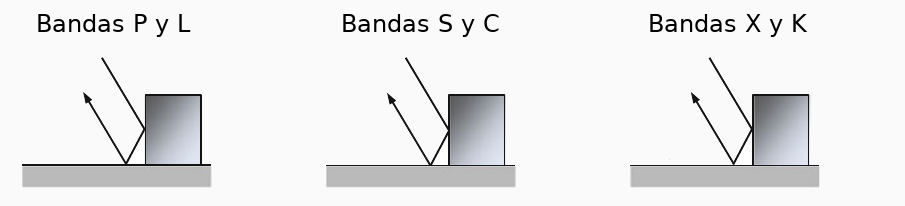
\includegraphics[width=\textwidth]{fig:interacciones-3.png}
      \caption{Interacciones entre los distintos blancos según la longitud de onda.}
      \label{}
    \end{figure}
\end{frame}
%--- Next Frame ---%




\begin{frame}{} \vskip0cm
    \begin{figure}
    \centering
    \subfloat[Banda C ($5.7cm$)]{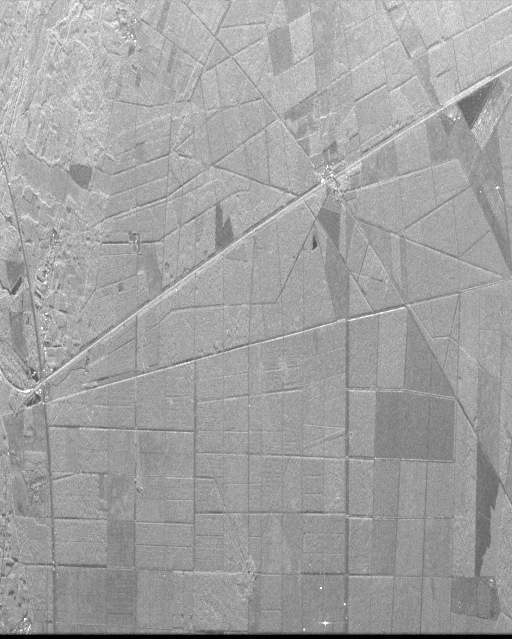
\includegraphics[width=0.2\textwidth]{fig:C.png}}\hspace{1cm}
    \subfloat[Banda L ($24cm$)]{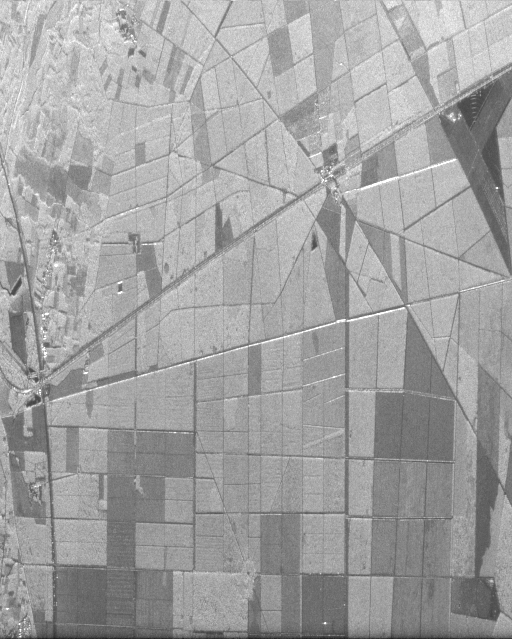
\includegraphics[width=0.2\textwidth]{fig:L.png}}\hspace{1cm}
    \subfloat[Banda P ($68cm$)]{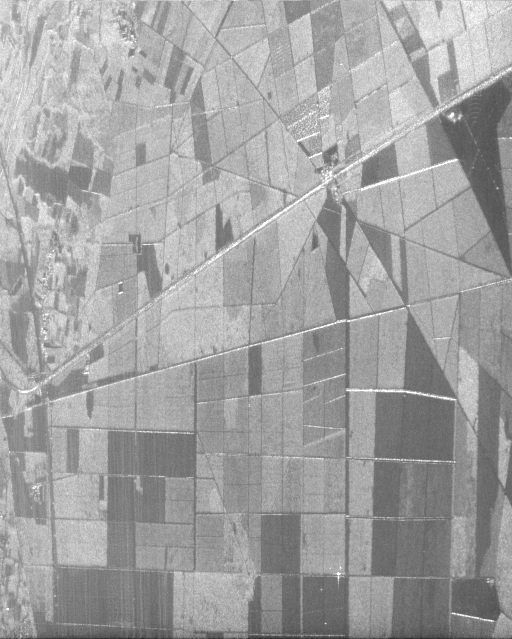
\includegraphics[width=0.2\textwidth]{fig:P.png}}
    \caption{Misma región vista en las bandas C, L y P.}
    \end{figure}
\end{frame}
%--- Next Frame ---%
\subsection{Resolución espacial}

\begin{frame}{} \vskip0cm
    A diferencia de la mayoría de los sistemas ópticos, los sistemas de radar tienen dos resoluciones:
    \begin{itemize}
      \item En rango, perdendicular a la dirección de movimiento del satélite.
      \item En acimut, paralelo a la dirección de movimiento del satélite.
    \end{itemize}
\end{frame}
%--- Next Frame ---%

\begin{frame}{} \vskip0cm
  Se calculan como:
    \begin{columns}
    \begin{column}{0.5\textwidth}
     \begin{block}{Resolución en rango}
      \begin{equation}
        \rho_{RG} = \frac{c}{2B}
      \end{equation}
     \end{block}
    \end{column}
    \begin{column}{0.5\textwidth}  %%<--- here
      \begin{block}{Resolución en azymuth}
        \begin{equation}
          \rho_{AZ} = \frac{L}{2}
        \end{equation}
      \end{block}
    \end{column}
    \end{columns}
    con $c$ la velocidad de la luz, $B$ el \emph{bandwidth} del sistema y $L$ la longitud de la antena.

    \begin{block}{Observación:}
      A diferencia de los satélites ópticos, la resolución en un sistema SAR no depende de la distancia entre el satélite y el blanco.
    \end{block}
\end{frame}
%--- Next Frame ---%


%\gracias
%--- Next Frame ---%

\section{Speckle y procesamiento}

\subsection{Speckle}

\begin{frame}{} \vskip0cm
  \begin{figure}
    \centering
    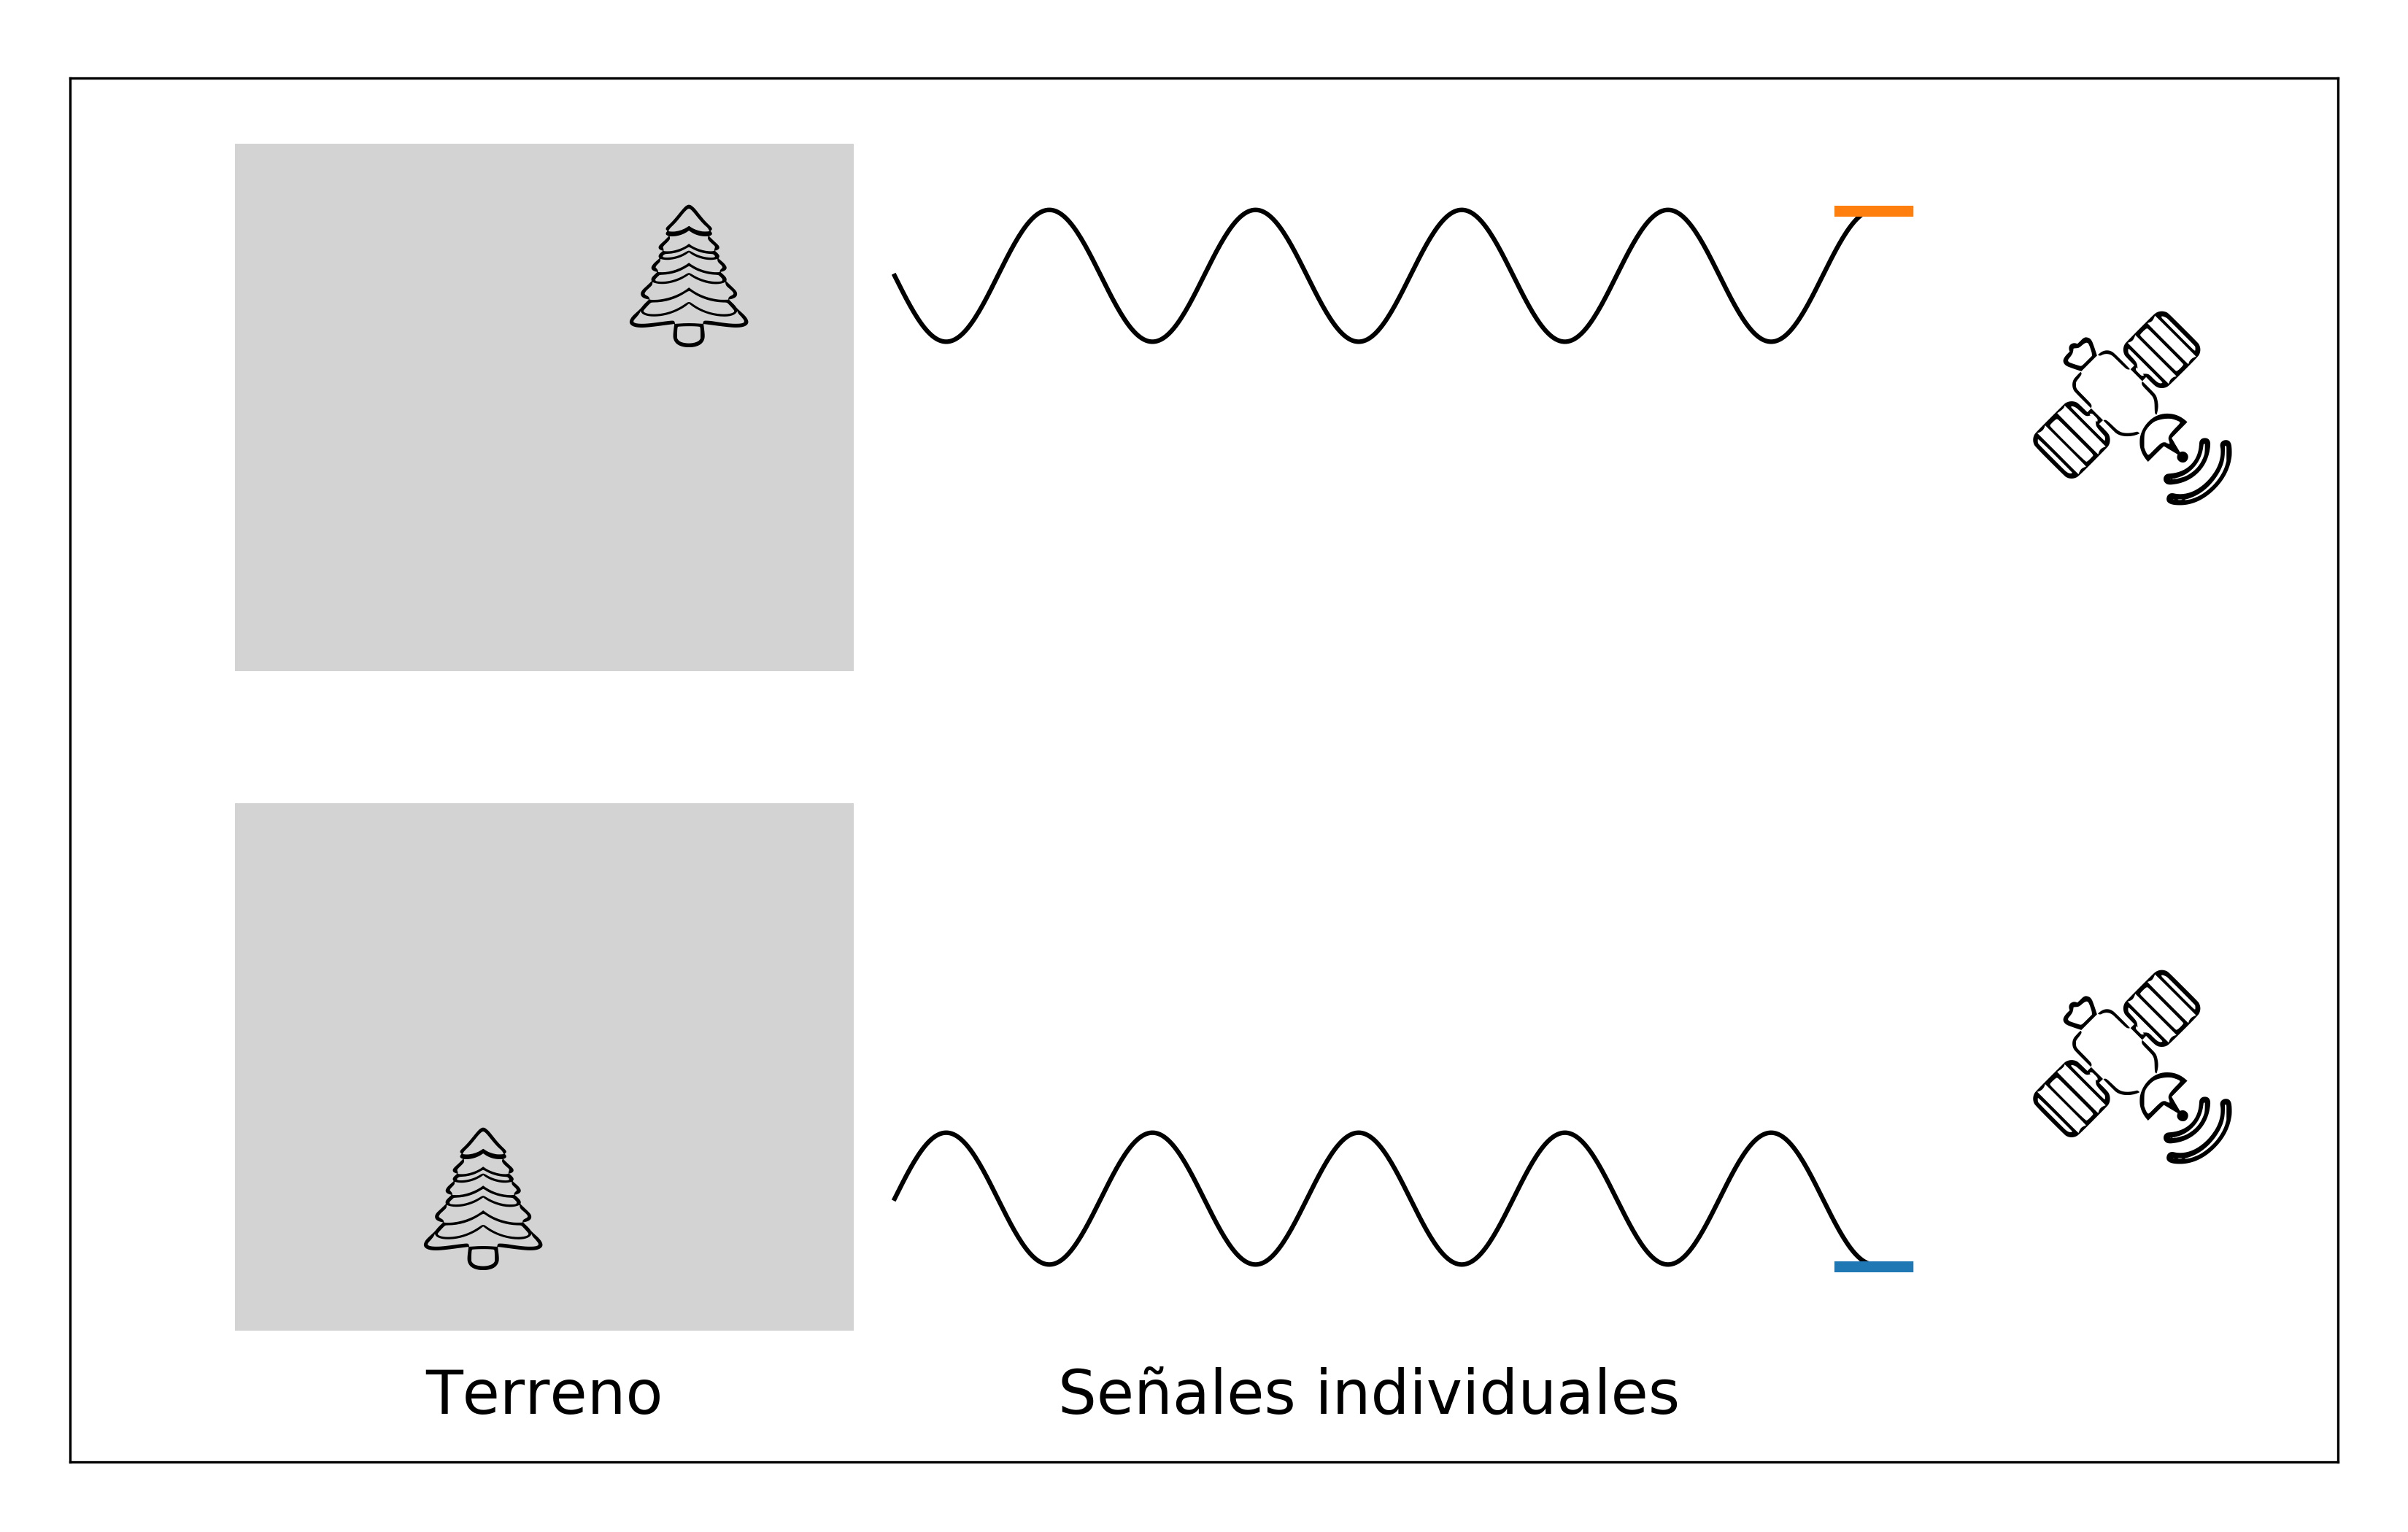
\includegraphics[width=0.65\textwidth]{fig:fase.png}
    \caption{Medición de fase y amplitud para un solo blanco.}
    \label{}
  \end{figure}
\end{frame}
%--- Next Frame ---%

\begin{frame}{} \vskip0cm
  \begin{figure}
    \centering
    \movie[width = 0.95\textwidth,loop,autostart]{\centering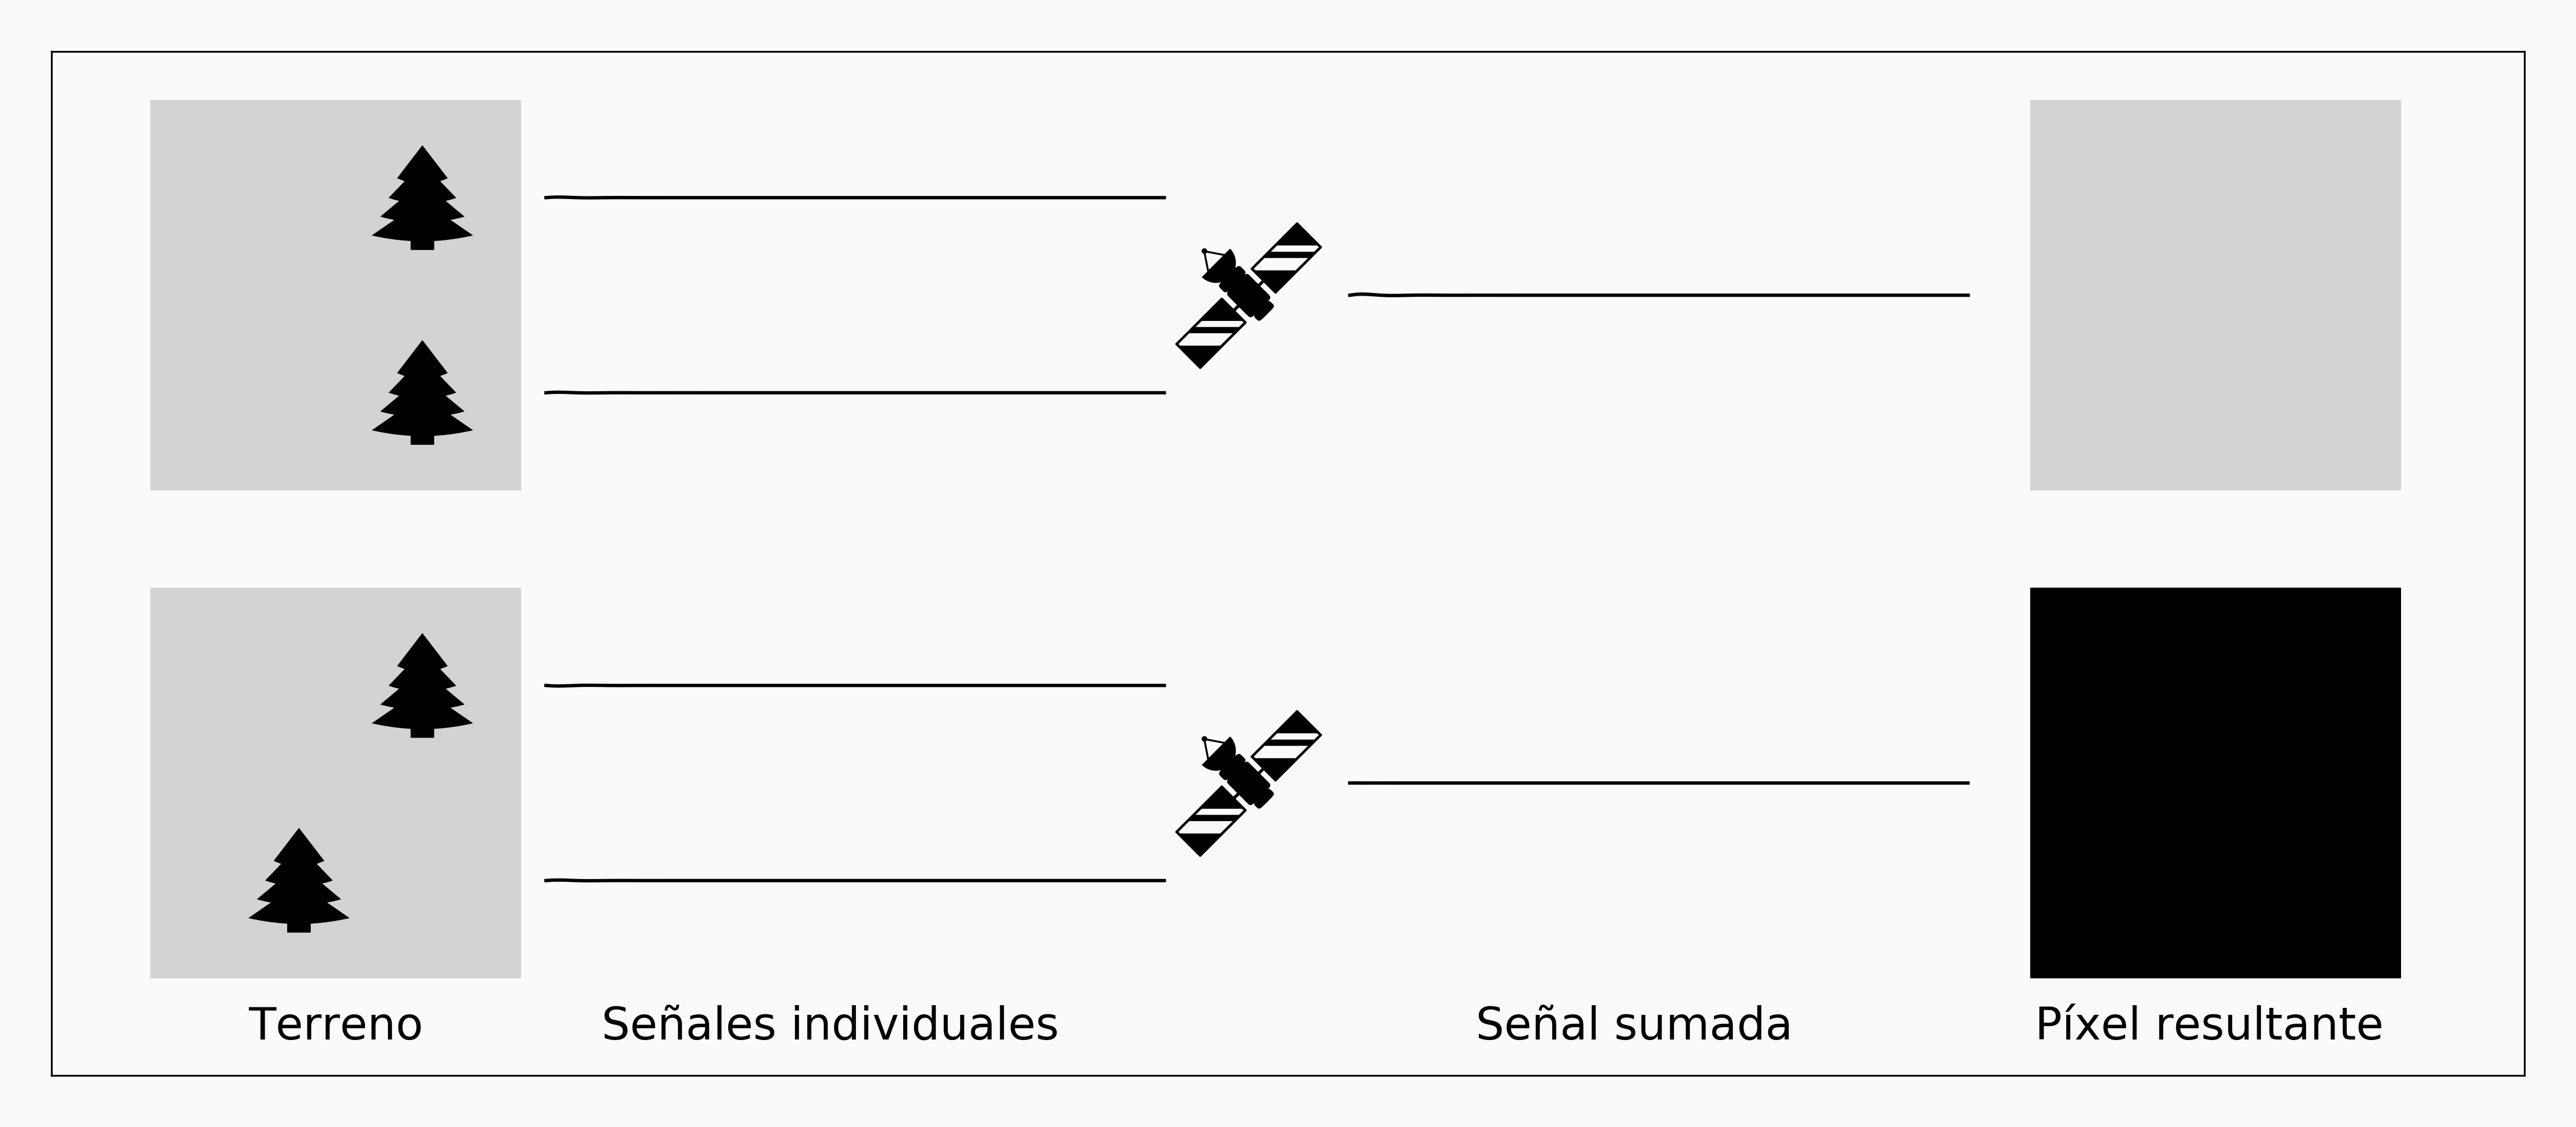
\includegraphics[width=0.95\textwidth]{fig:speckle.png}}{./figs/fig:speckle.mp4}
    \caption{Medición de fase y amplitud con varios blancos dentro del píxel.}
    \label{}
  \end{figure}
\end{frame}
%--- Next Frame ---%


\begin{frame}{} \vskip0cm
  \begin{itemize}
    \item El specke no es ruido, es determinístico. Si repito la adquisición manteniendo la geometría el patrón de specke resulta idéntico.
    \item Si promedio dos pixeles en amplitud tendré el mismo problema. Tengo que promediarlos en potencia (multilooking)
  \end{itemize}
      \begin{figure}
        \centering
        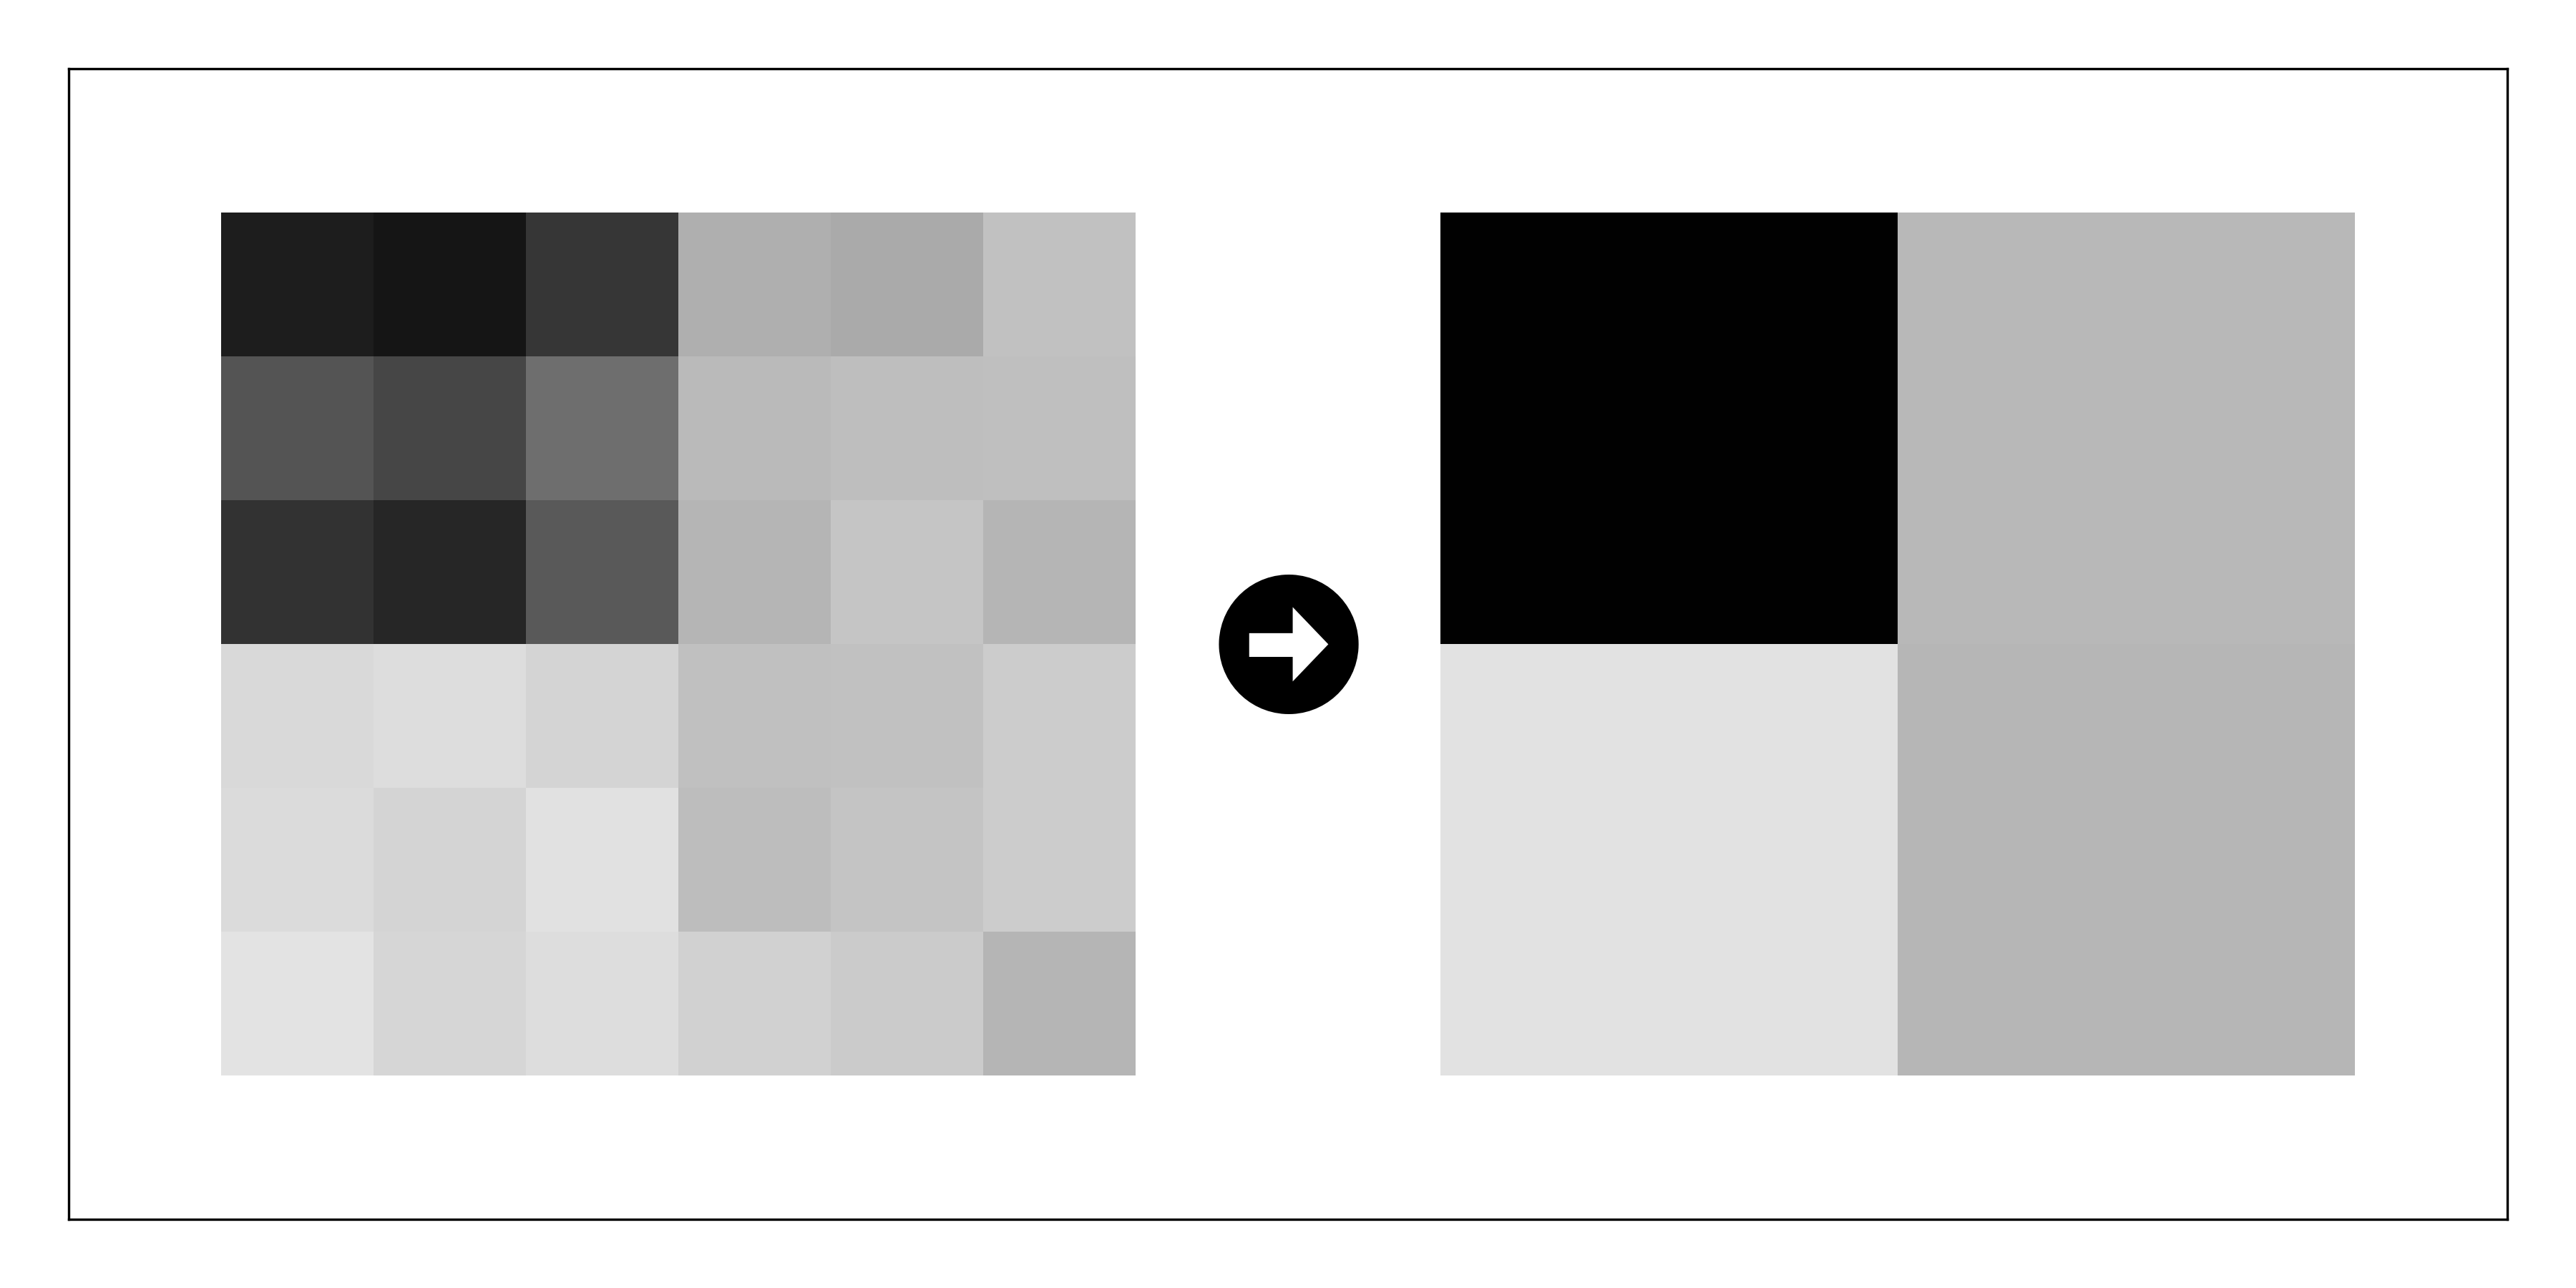
\includegraphics[width=0.65\textwidth]{fig:multilook.png}
        %\caption{Proceso de multilook.}
        \label{}
      \end{figure}

\end{frame}
%--- Next Frame ---%


\begin{frame}{} \vskip0cm

   \begin{block}{Multilook}
     \begin{itemize}
       \item Se promedian en potencia varios píxeles vecinos y se los asigna a uno nuevo
       \item Se pierde resolución.
       \item Efectivo contra el speckle.
     \end{itemize}
   \end{block}

\end{frame}
%--- Next Frame ---%

\begin{frame}{} \vskip0cm
  \begin{columns}
  \begin{column}{0.5\textwidth}
    \begin{figure}
      \centering
      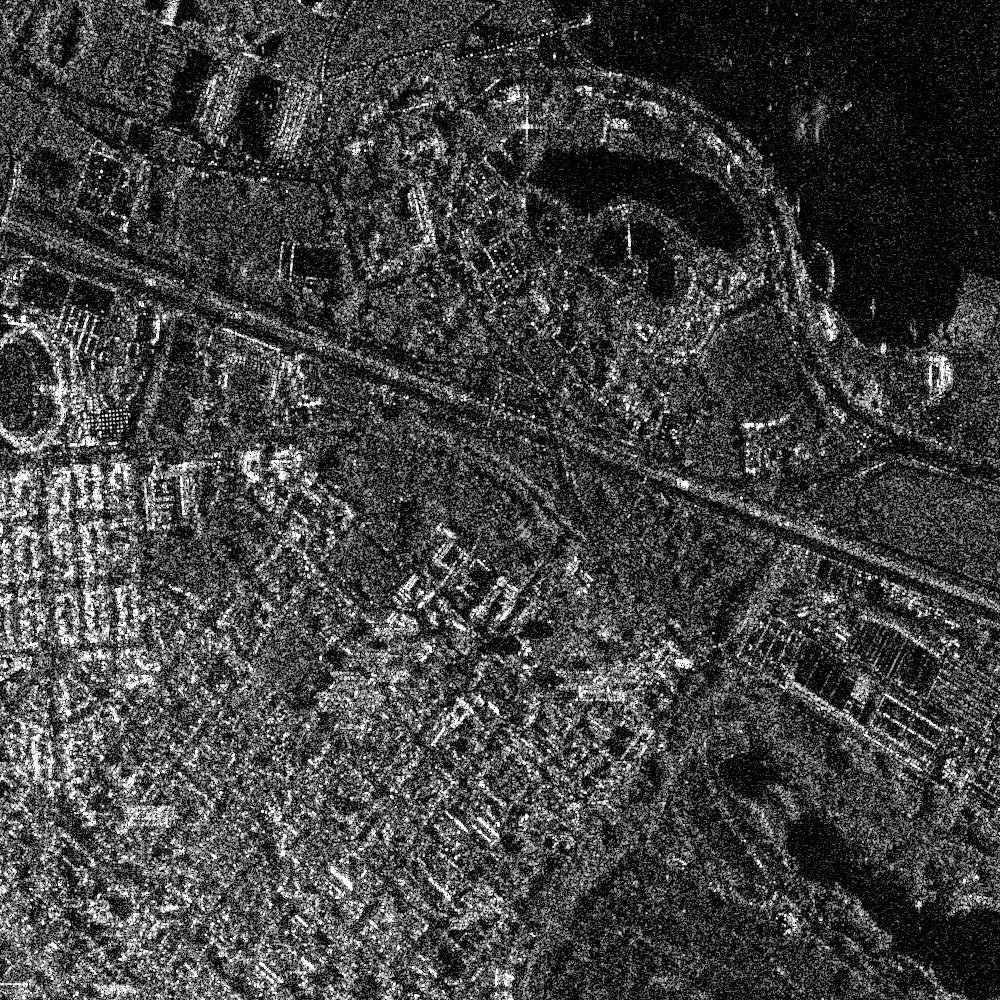
\includegraphics[width=0.8\textwidth]{fig:original.jpg}
      \caption{Imagen original.}
      \label{}
    \end{figure}
  \end{column}
  \begin{column}{0.5\textwidth}  %%<--- here
    \begin{figure}
      \centering
      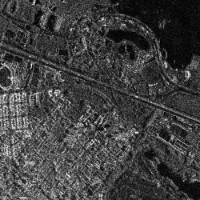
\includegraphics[width=0.8\textwidth]{fig:multilook.jpg}
      \caption{Imagen multilookeada.}
      \label{}
    \end{figure}
  \end{column}
  \end{columns}
\end{frame}
%--- Next Frame ---%


\subsection{Distorciones geométricas}

\begin{frame}{} \vskip0cm
      \begin{figure}
        \centering
        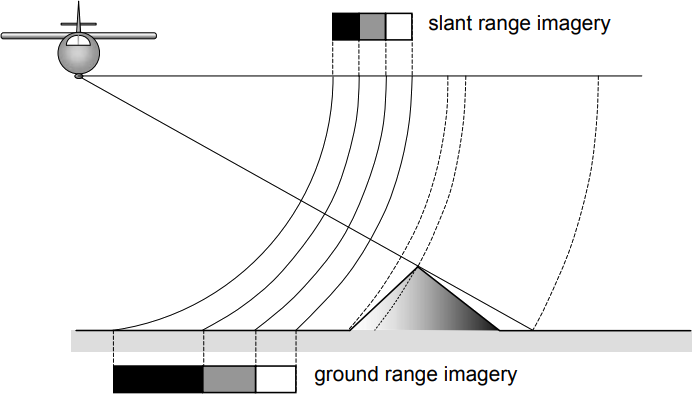
\includegraphics[width=0.8\textwidth]{fig:slant.png}
        \caption{Comparación entre Slant range y Ground range.}
        \label{}
      \end{figure}
\end{frame}
%--- Next Frame ---%

\begin{frame}{} \vskip0cm
      \begin{figure}
        \centering
        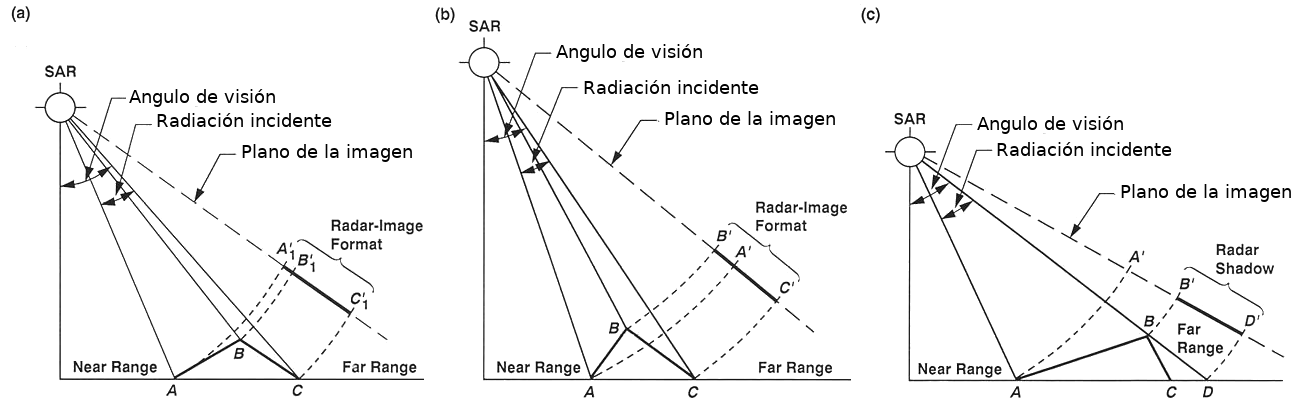
\includegraphics[width=\textwidth]{fig:dist.png}
        \caption{Distorciones geométricas típicas en una imagen radar:\\ {\centering a. foreshortening, b. layover, c. shadowing.}}
        \label{}
      \end{figure}
\end{frame}
%--- Next Frame ---%

\begin{frame}{} \vskip0cm
    \begin{figure}
      \centering
      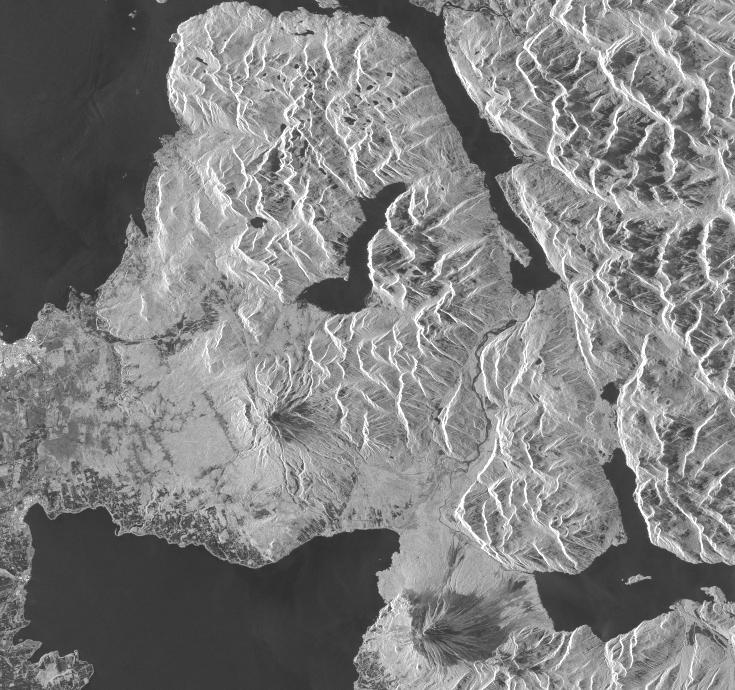
\includegraphics[width=0.5\textwidth]{fig:dist2.jpg}
      \caption{Vista de una imagen radar sin correcciones geométricas.}
      \label{}
    \end{figure}
\end{frame}
%--- Next Frame ---%

\begin{frame}{} \vskip0cm
  \begin{block}{Correcciones geométricas}
    Para resolver parte de las distorciones geométricas es util pasar la imagen del \emph{slant range} al \emph{ground range}. Para esto deberemos proyectarla y podemos hacerlo de dos maneras
    \begin{itemize}
      \item Sobre el elipsoide.
      \item Sobre un modélo de elevación digital.
    \end{itemize}
  \end{block}
\end{frame}
%--- Next Frame --- %

\subsection{Niveles de procesamiento}
\begin{frame}{} \vskip0cm
  % Please add the following required packages to your document preamble:
  % \usepackage{booktabs}
  % \usepackage{graphicx}
  \begin{table}[]
  \centering
  \resizebox{\textwidth}{!}{%
  \begin{tabular}{@{}cccc@{}}
  \toprule
  L1A (SLC)                                                                                                    & L1B (GRD)                                                                  & L1C (GEC)                                                                              & L1D (GTC)                                                                                     \\ \midrule
  Single Look Complex                                                                                          & Ground Range Detected                                                      & Geocoded Elipsoid Corrected                                                            & Geocoded Terrain Corrected                                                                    \\
  \multicolumn{1}{p{4.5cm}}{Datos en formato complejo (real e imaginario), sin multilook y en la geometria del radar} & \multicolumn{1}{p{4.5cm}}{Datos en potencia, con multilook y proyectada al suelo} & \multicolumn{1}{p{4.5cm}}{Datos en potencia, con multilook y geocodificada sobe el elipsoide} & \multicolumn{1}{p{4.5cm}}{Datos en potencia, con multilook y geocodificada sobe el el terreno (DEM)}\\
    \multicolumn{1}{p{4.5cm}}{
\includegraphics[width=4.3cm]{fig:l1a.png}} & \multicolumn{1}{p{4.5cm}}{
\includegraphics[width=4.3cm]{fig:l1b.png}} & \multicolumn{1}{p{4.5cm}}{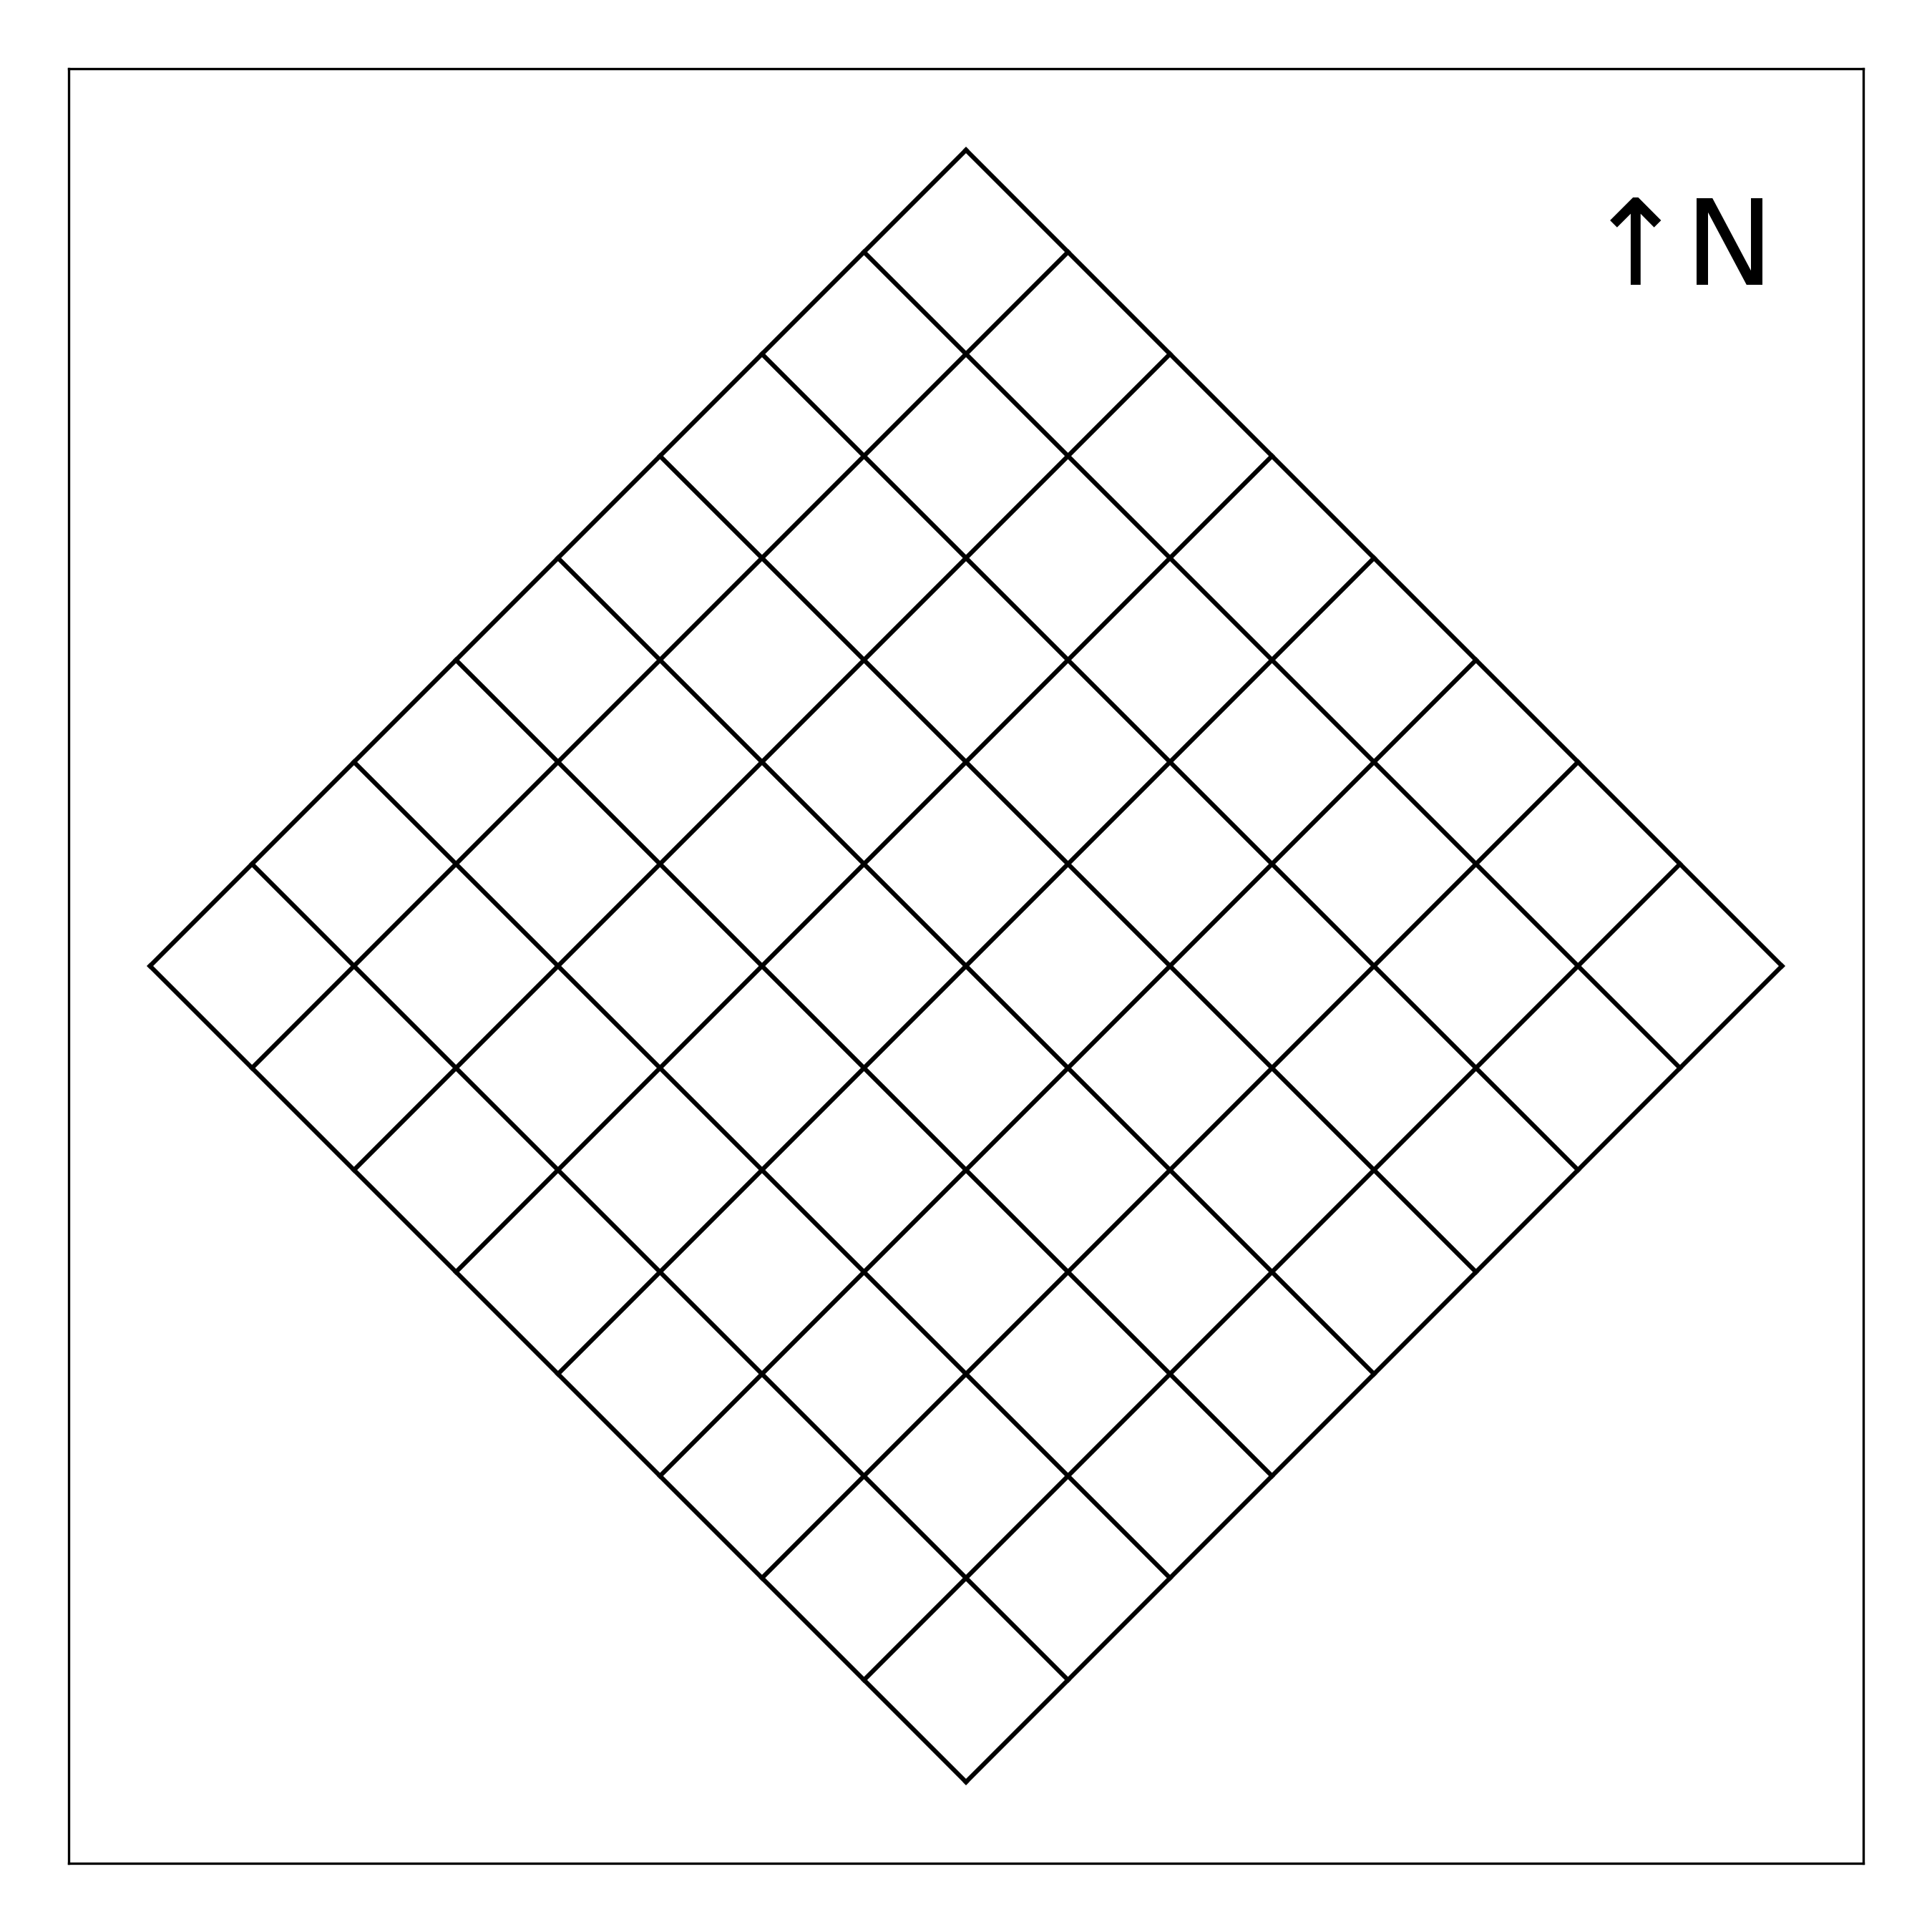
\includegraphics[width=4.3cm]{fig:l1c.png}} & \multicolumn{1}{p{4.5cm}}{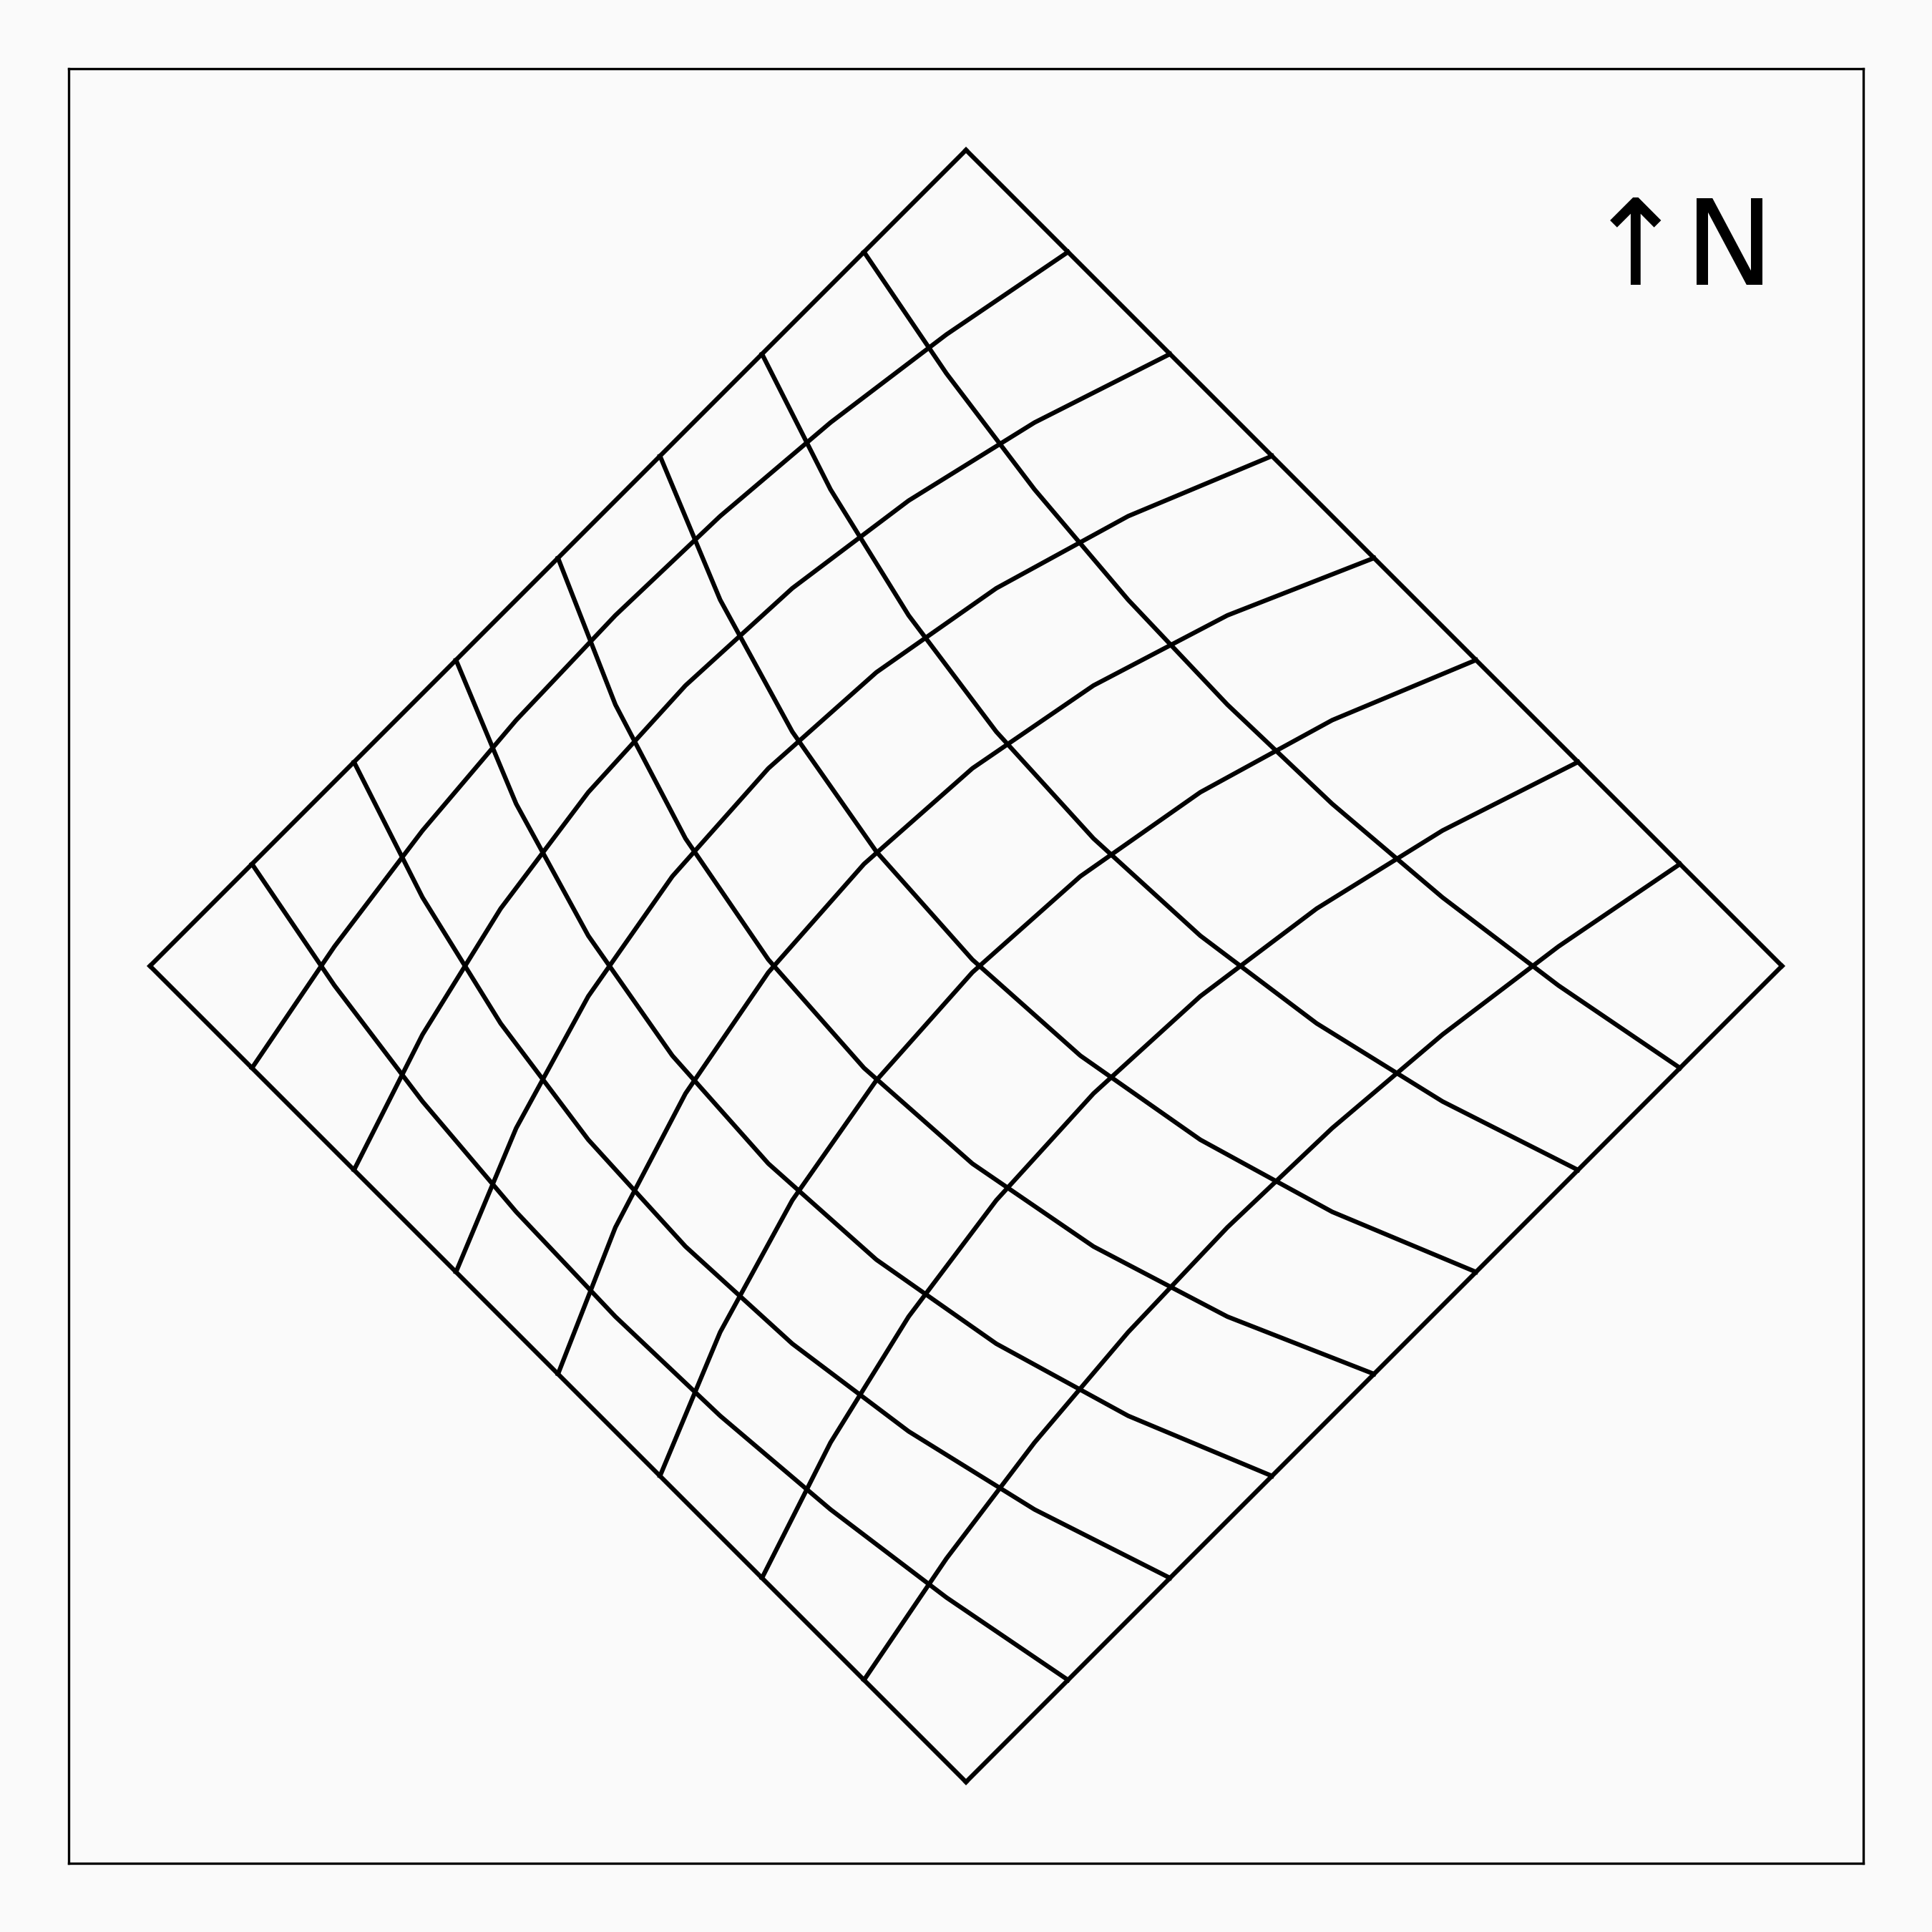
\includegraphics[width=4.3cm]{fig:l1d.png}}\\
    \bottomrule
  \end{tabular}%
  }
  \caption{Niveles de procesamiento típicos para una imagen SAR.}
  \label{my-label}
  \end{table}
\end{frame}

\gracias
%--- Next Frame ---%

\section{Polarimetría}

\subsection{Ecuación de radar}

\begin{frame}{} \vskip0cm
    \begin{block}{Definición}
      \begin{equation}
        P_r \pause \sim \frac{ P_t \pause G_t \pause G_r \pause \lambda^2 \pause \sigma}{\pause R^4}
      \end{equation}
    \end{block}
\end{frame}
%--- Next Frame ---%

\begin{frame}{} \vskip0cm
    \begin{block}{Definición}
      \begin{equation}
        P_r = \frac{ P_t  G_t  G_r  \lambda^2  \sigma}{ (4\pi)^3 \ R^4}
      \end{equation}
      Con $P_r$ y $P_t$ las potencias recibidas y transmitidas, $G_r$ y $G_t$ las ganancias del emisor y receptor, $\lambda$ la longitud de onda, $\sigma$ el coeficiente de backscatter o retrodisperción y $R$ la distancia entre el emisor y el blanco.
    \end{block}
\end{frame}
%--- Next Frame ---%

\begin{frame}{} \vskip0cm

  \begin{block}{Definición}
    Definimos el coeficiente de retrodispersión por unidad de área de un radar como
    \begin{equation}
      \sigma^0 = \frac{\sigma}{A}
    \end{equation}
    donde $\sigma$ es el coeficiente de retrodispersión y $A$ el área del píxel.
  \end{block}
  \pause
    \begin{block}{Definición}
      Es común expresar el coeficiente de retrodispersión por unidad de área como
      \begin{equation}
        \sigma^0 [dB] = 10\log_{10}(\sigma^0).
      \end{equation}
    \end{block}
%\pause
    %\begin{block}{Definición}
    %  Es común expresar el coeficiente de retrodispersión de un radar en decibels cómo
    %  \begin{equation}
    %    \sigma [dB] = 10\log_{10}(\sigma)
    %  \end{equation}
    %  donde $\sigma$ es el coeficiente de retrodispersión.
    %\end{block}
\end{frame}
%--- Next Frame ---%

\subsection{Polarización}

\begin{frame}{} \vskip0cm
  \begin{figure}
    \centering
    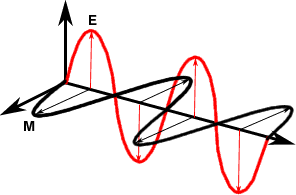
\includegraphics[width=0.5\textwidth]{fig:onda.png}
    \caption{Una onda electromagnética es una oscilación en el campo electromagnético, puede estar orientada en distintas direcciones, llamadas estado de polarización.}
    \label{}
  \end{figure}
\end{frame}
%--- Next Frame ---%

\begin{frame}{} \vskip0cm
  \begin{figure}
    \centering
    \movie[width = 0.8\textwidth,loop,autostart]{\centering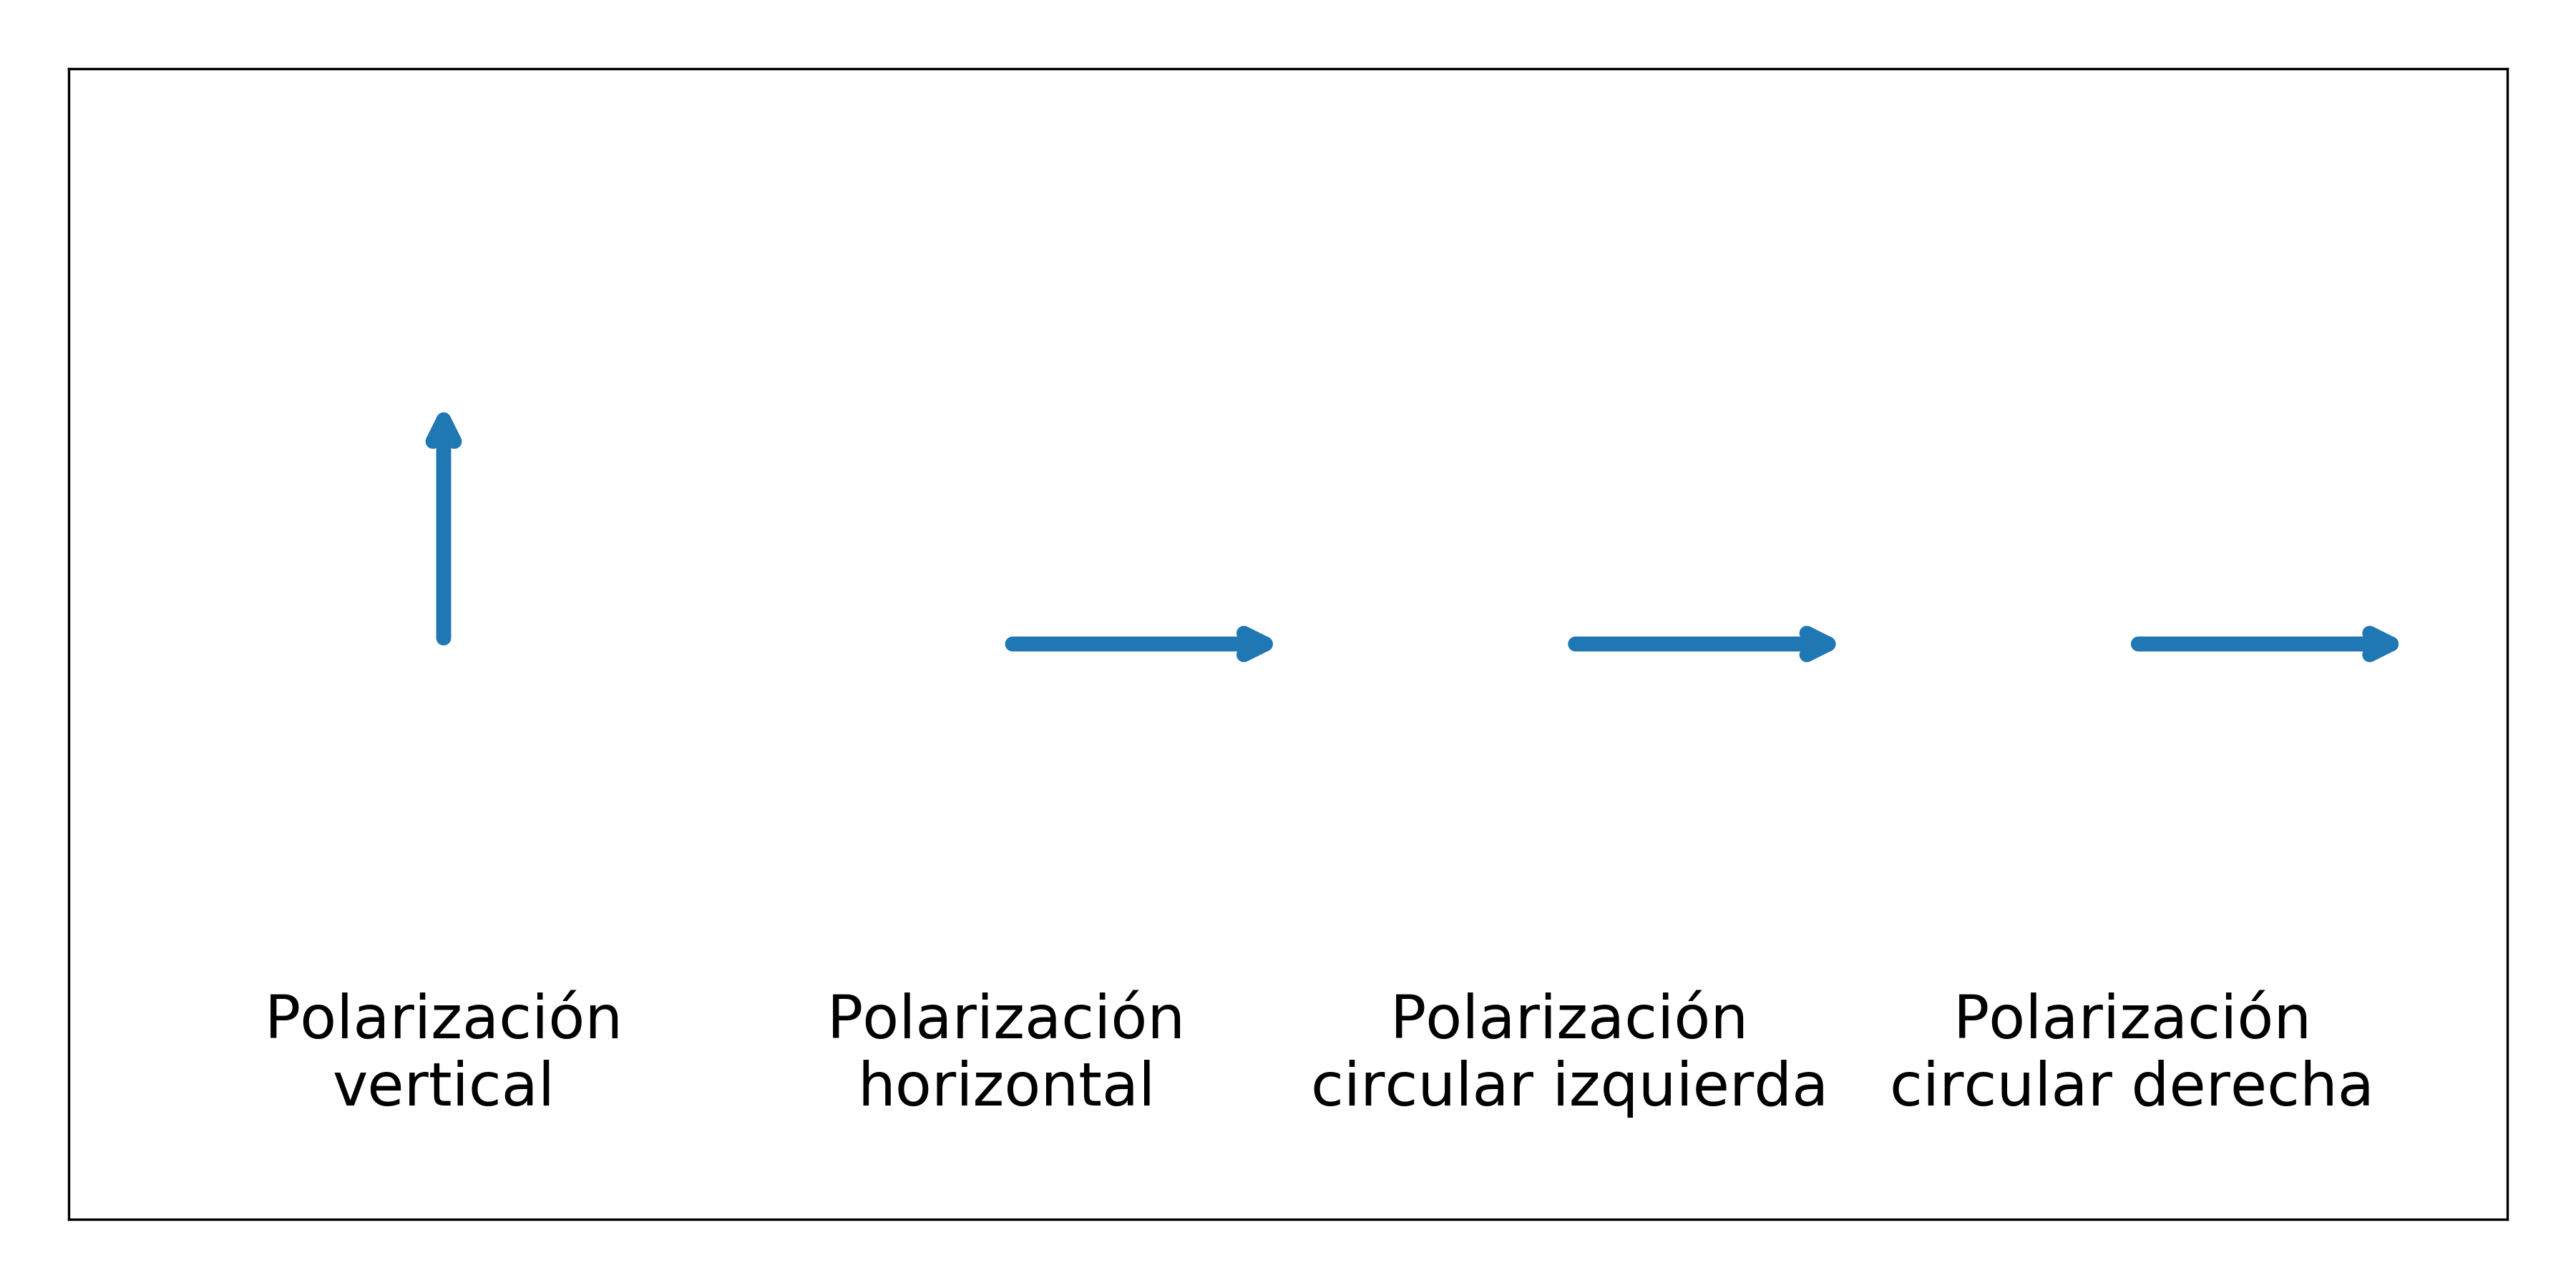
\includegraphics[width=0.8\textwidth]{fig:polarizado.png}}{../figs/fig:polarizado.mp4}
    \caption{Entre los estados de polarización más típicos se pueden destacar la polarización lineal y la circular.}
    \label{}
  \end{figure}
\end{frame}
%--- Next Frame ---%



\begin{frame}{} \vskip0cm
  \begin{figure}
    \centering
    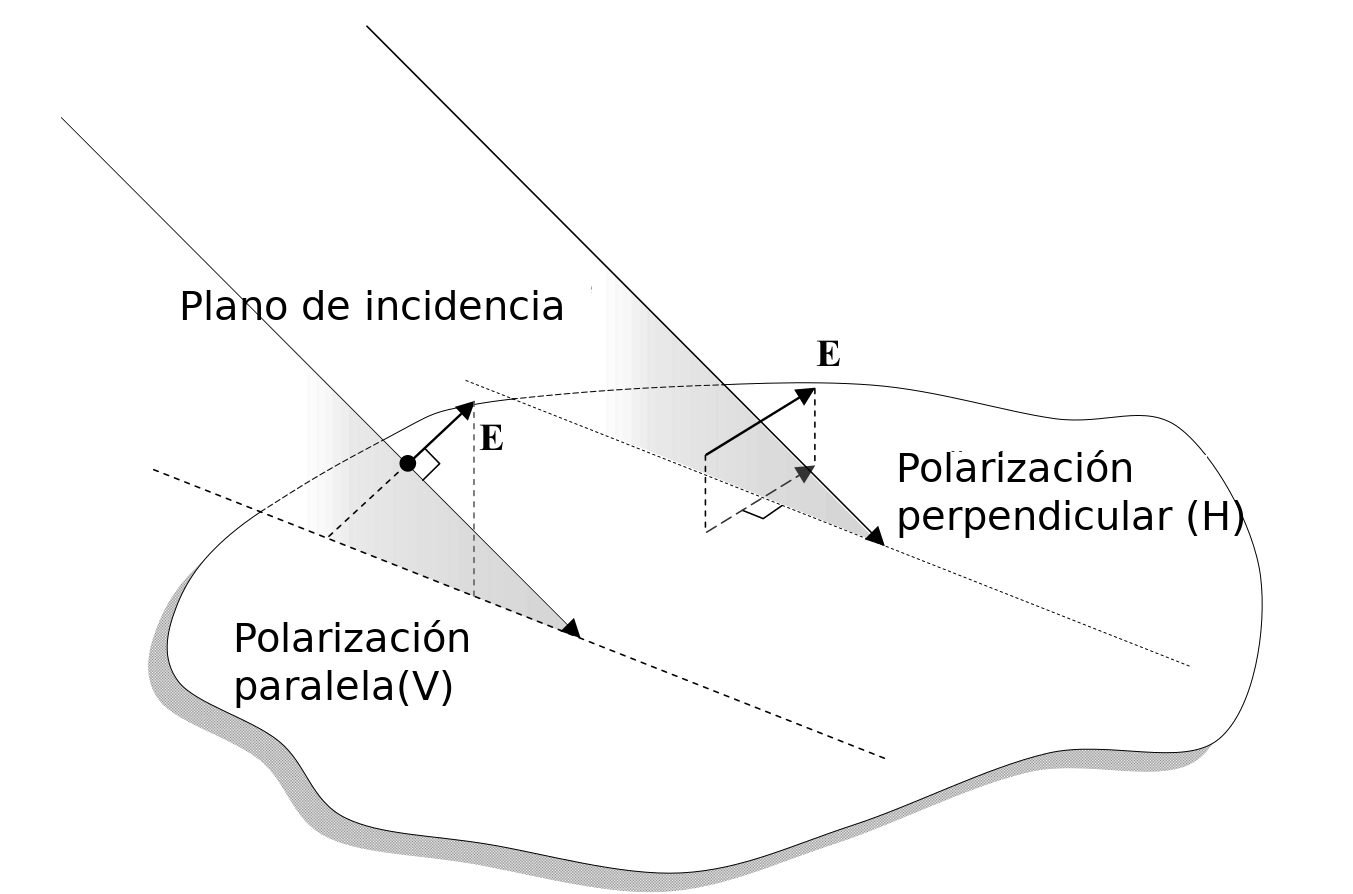
\includegraphics[width=0.55\textwidth]{fig:polarizacion.png}
    \caption{Algunos SAR pueden emitir y recibir tanto en H (Horizontal) -perpendicular al plano de incidencia-, como en V (Vertical) -paralela al plano de incidencia-. Combinándolas entre transmisión y recepción se obtienen 4 combinaciones polarimétricas: {\bf HH, HV, VH, y VV}.}
    \label{}
  \end{figure}
\end{frame}
%--- Next Frame ---%

\begin{frame}{} \vskip0cm
  \begin{figure}
    \centering
    \subfloat[Polarización HH]{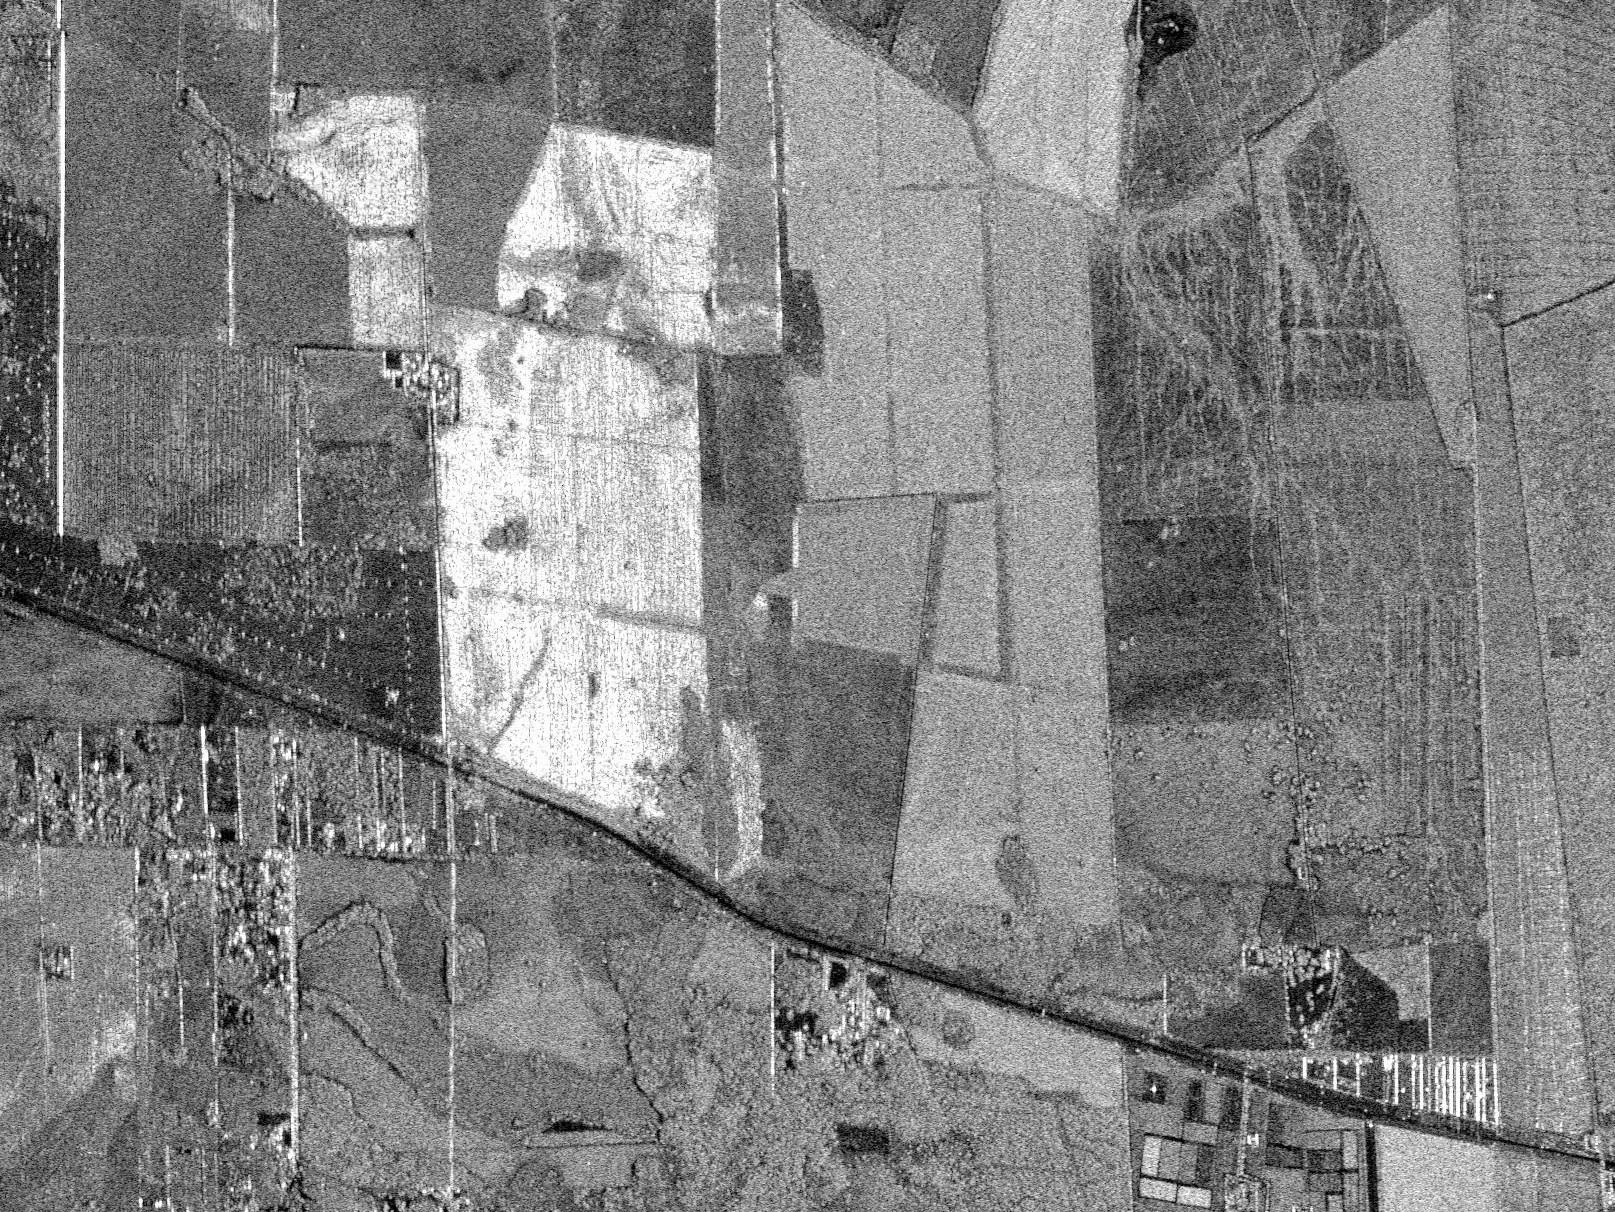
\includegraphics[width=0.25\textwidth]{fig:HH.jpg}}\hspace{1cm}
    \subfloat[Polarización HV]{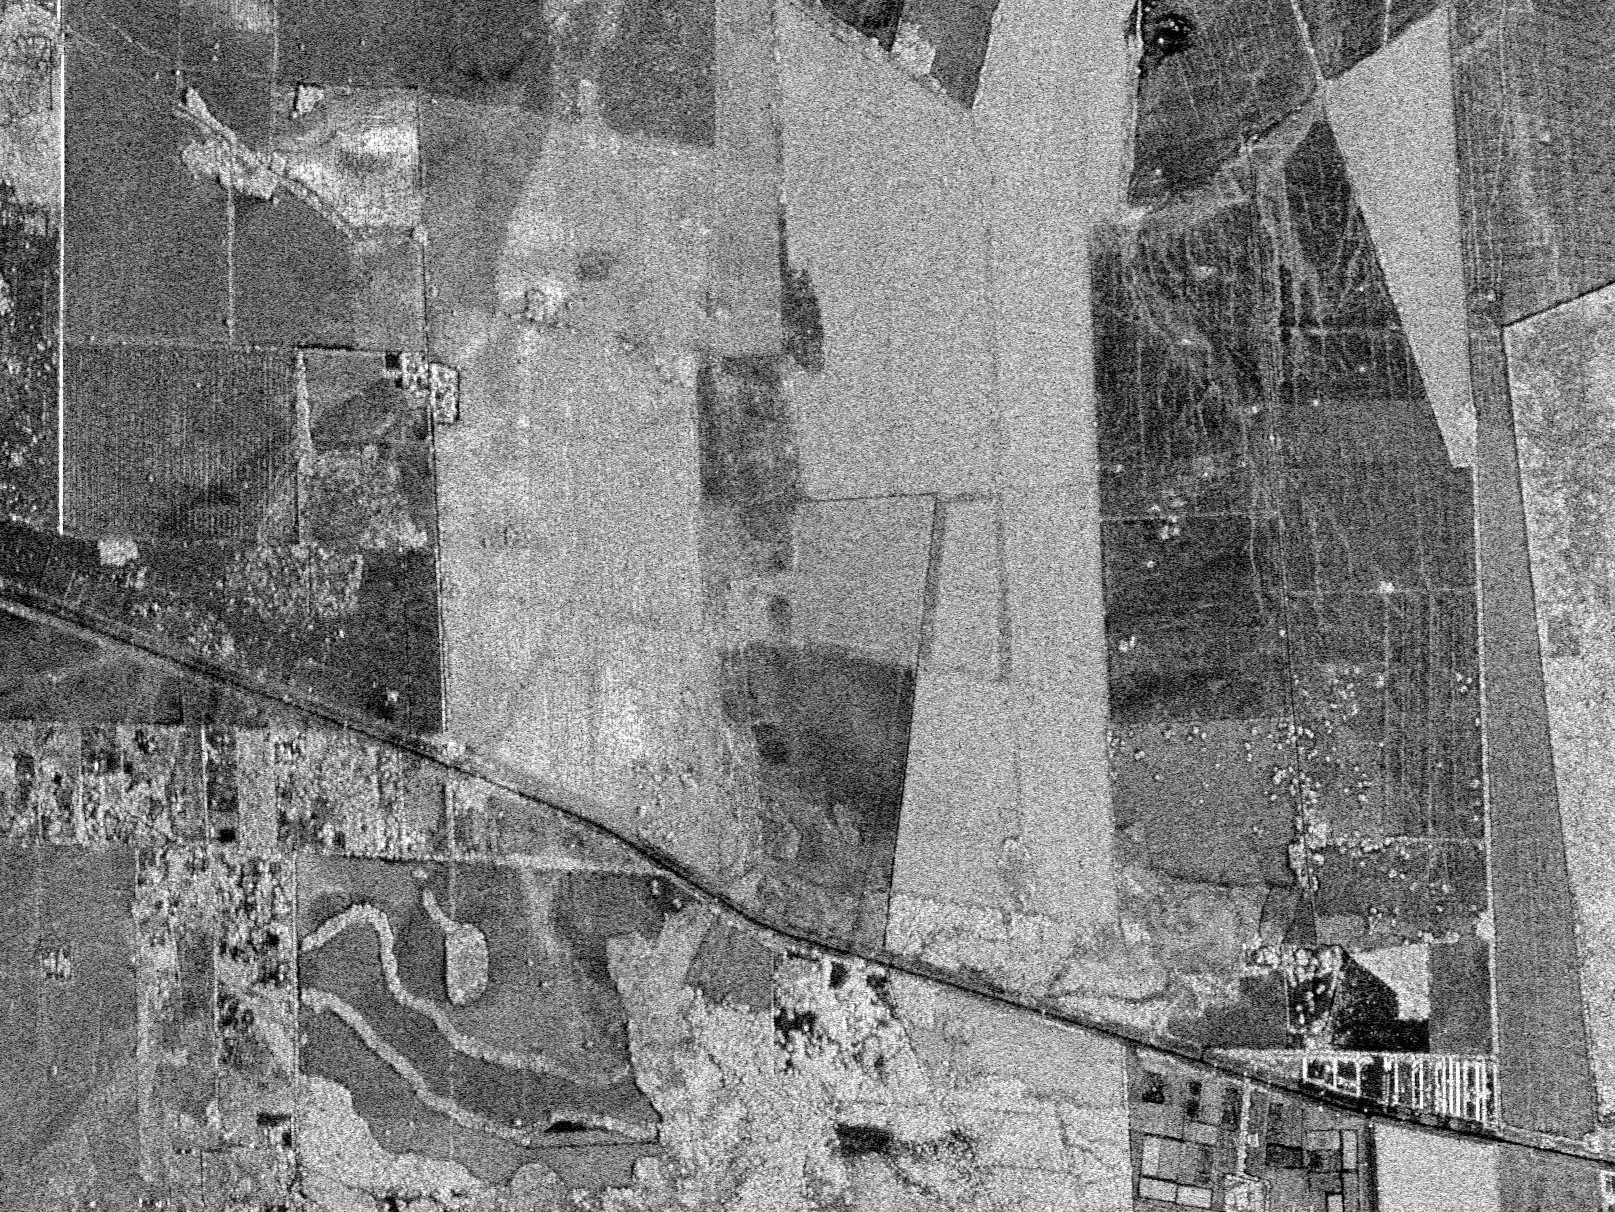
\includegraphics[width=0.25\textwidth]{fig:HV.jpg}}
    \\
    \subfloat[Polarización VH]{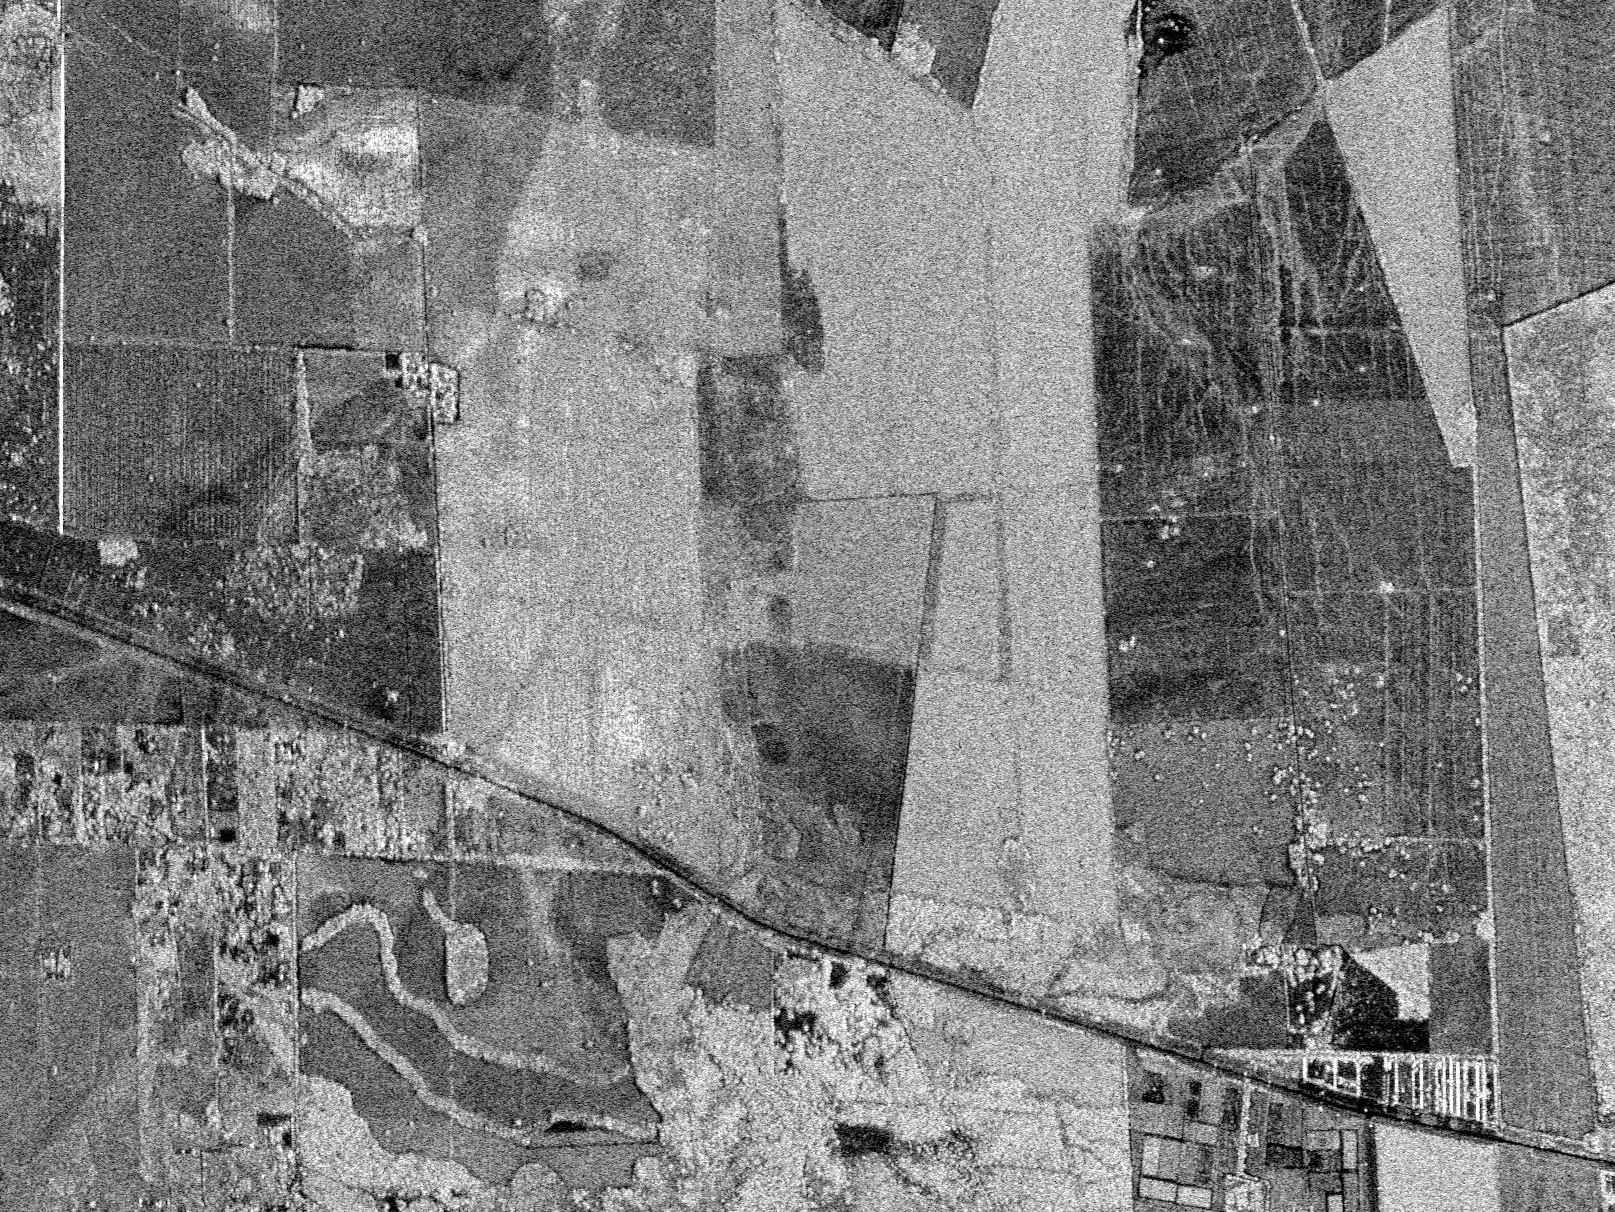
\includegraphics[width=0.25\textwidth]{fig:VH.jpg}}\hspace{1cm}
    \subfloat[Polarización VV]{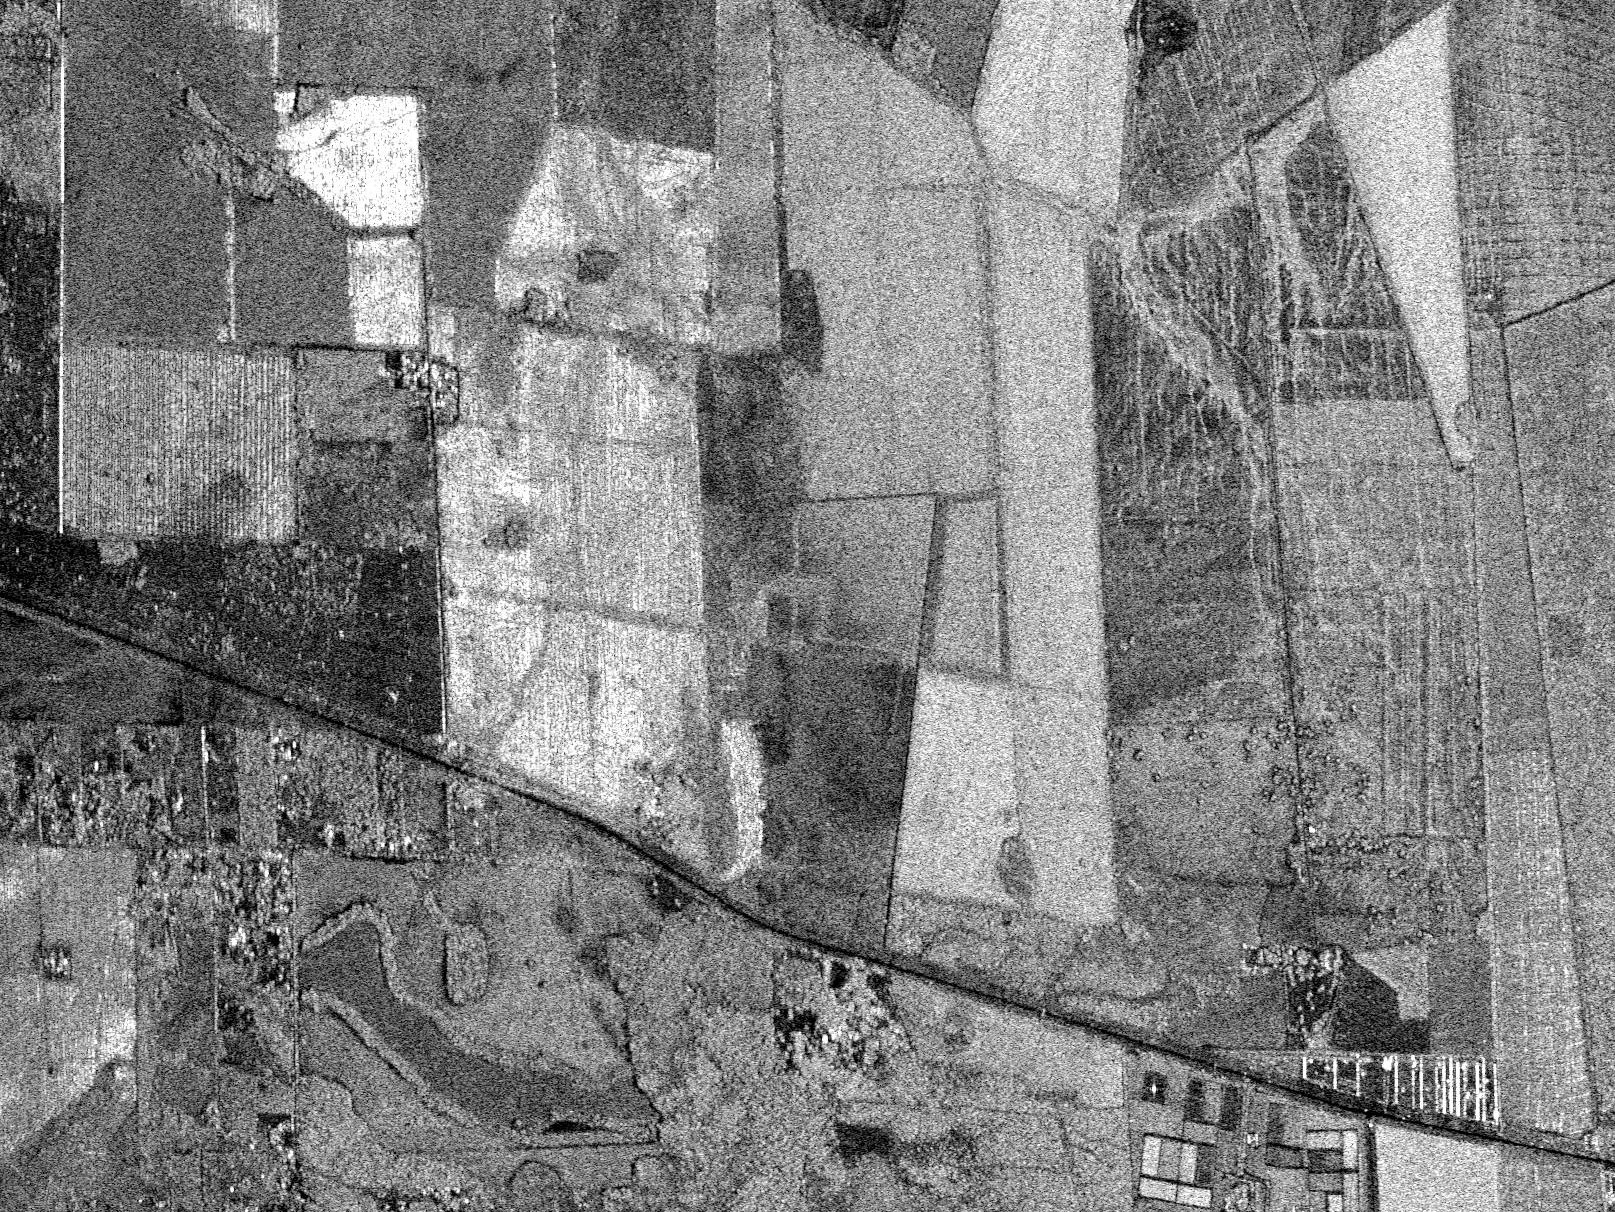
\includegraphics[width=0.25\textwidth]{fig:VV.jpg}}
    \caption{Distintas polarizaciones para una misma región.}
  \end{figure}
\end{frame}
%--- Next Frame ---%

%\begin{frame}{} \vskip0cm
%  En este caso la representación del coeficiente de backscatter es matricial
%  \begin{columns}
%    \begin{column}{0.5\textwidth}
%     \begin{block}{Matriz de scattering}
%      \begin{equation}
%        S=
%  \begin{bmatrix}
%    S_{HH} & S_{HV} \\
%    S_{VH} & S_{VV}
%  \end{bmatrix}
%      \end{equation}
%     \end{block}
%    \end{column}
%    \begin{column}{0.5\textwidth}  %%<--- here
%      \begin{block}{Matriz de backscatter}
%        \begin{equation}
%          \sigma_0= \frac{1}{A}
%  \begin{bmatrix}
%    |S_{HH}|^2 & |S_{HV}|^2 \\
%    |S_{VH}|^2 & |S_{VV}|^2
%  \end{bmatrix}
%        \end{equation}
%        con $A$ el area del píxel.
%      \end{block}
%    \end{column}
%    \end{columns}
%\end{frame}
%--- Next Frame ---%

\subsection{Descoposición de Pauli}

\begin{frame}{} \vskip0cm
     \begin{block}{Descomposición de Pauli}
      \begin{equation}
        R = \left(\frac{HH-VV}{\sqrt{2}}\right)^2
      \end{equation}
      \begin{equation}
        G = \left(\sqrt{2}HV\right)^2
      \end{equation}
      \begin{equation}
        B = \left(\frac{HH+VV}{\sqrt{2}}\right)^2
      \end{equation}
     \end{block}
    La descomposición de Pauli es una manera de visualizar los distintos mecanismo de scattering presentes: azul -especular-, verde -en volumen- y rojo -doble rebote-.
\end{frame}
%--- Next Frame ---%

\begin{frame}{} \vskip0cm
  \begin{figure}
    \centering
    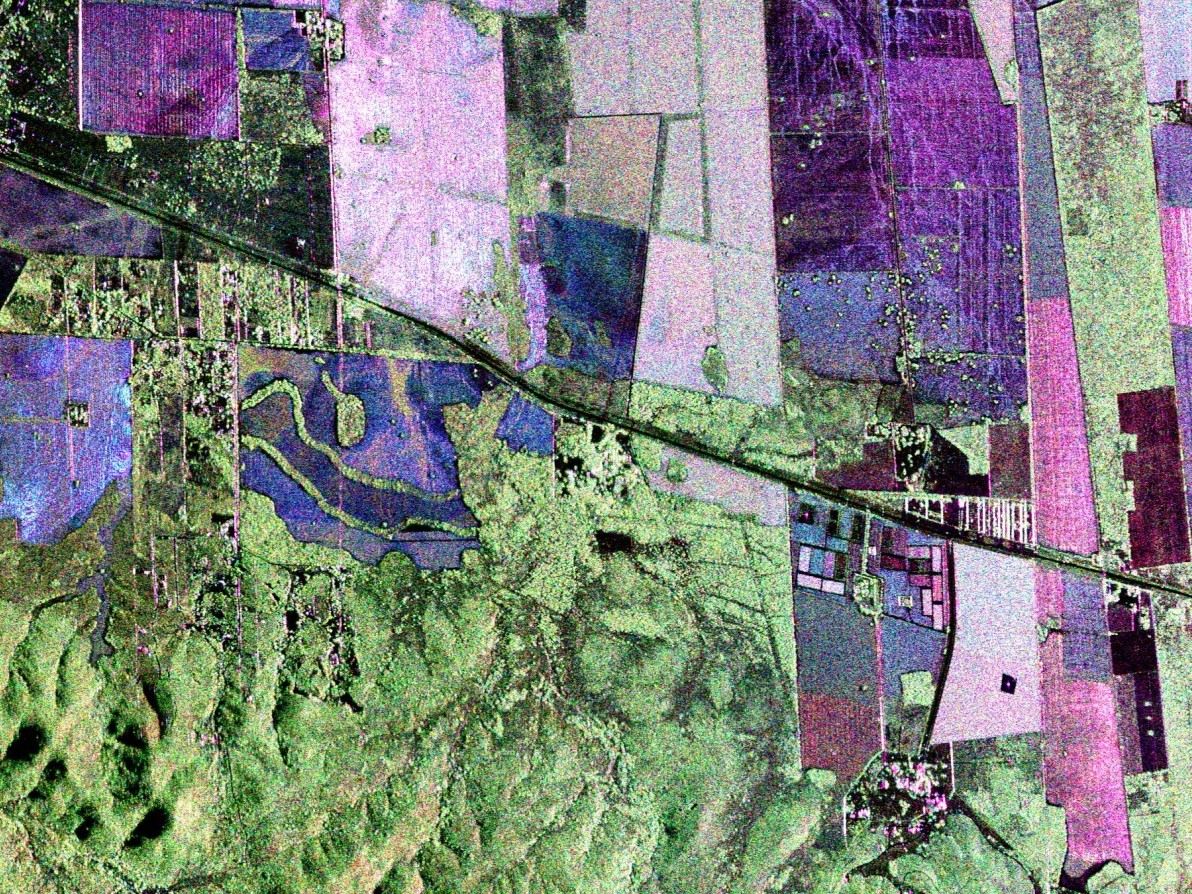
\includegraphics[width=0.5\textwidth]{fig:rgbpauli}
    \caption{Descomposición de Pauli en combinación RGB.}
    \label{}
  \end{figure}
\end{frame}
%--- Next Frame ---%

%\gracias
%--- Next Frame ---%

\section{Misión SAOCOM y aplicaciones}
\subsection{Misión SAOCOM}

\begin{frame}{} \vskip0cm
  \begin{figure}
    \centering
    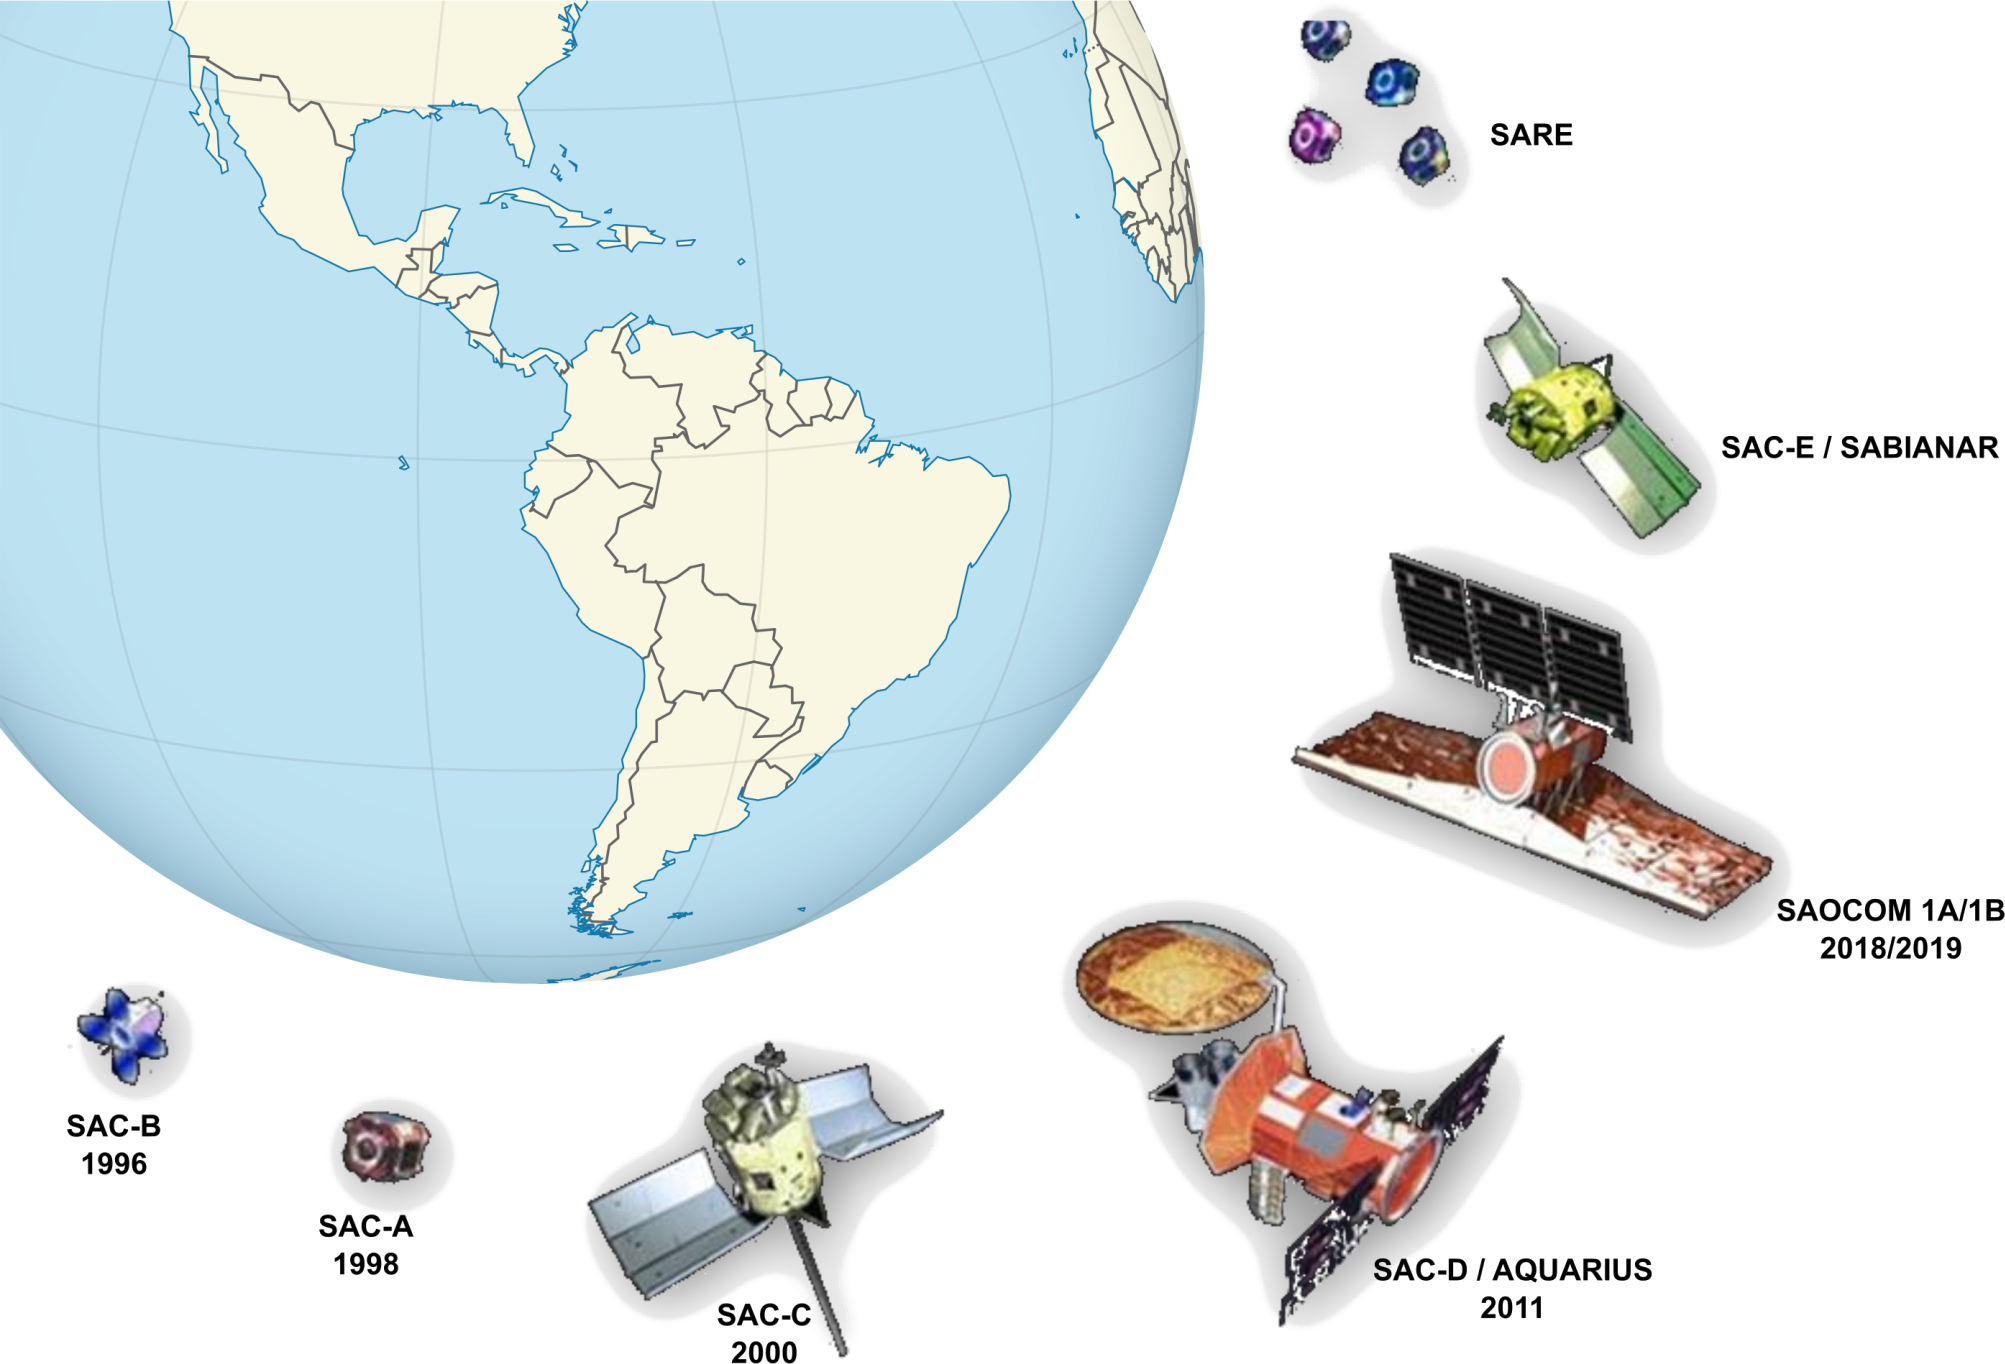
\includegraphics[width=0.65\textwidth]{fig:plan}
    \caption{Satélites del plan espacial nacional.}
    \label{}
  \end{figure}
\end{frame}
%--- Next Frame ---%

\begin{frame}{} \vskip0cm
  \begin{figure}
    \centering
    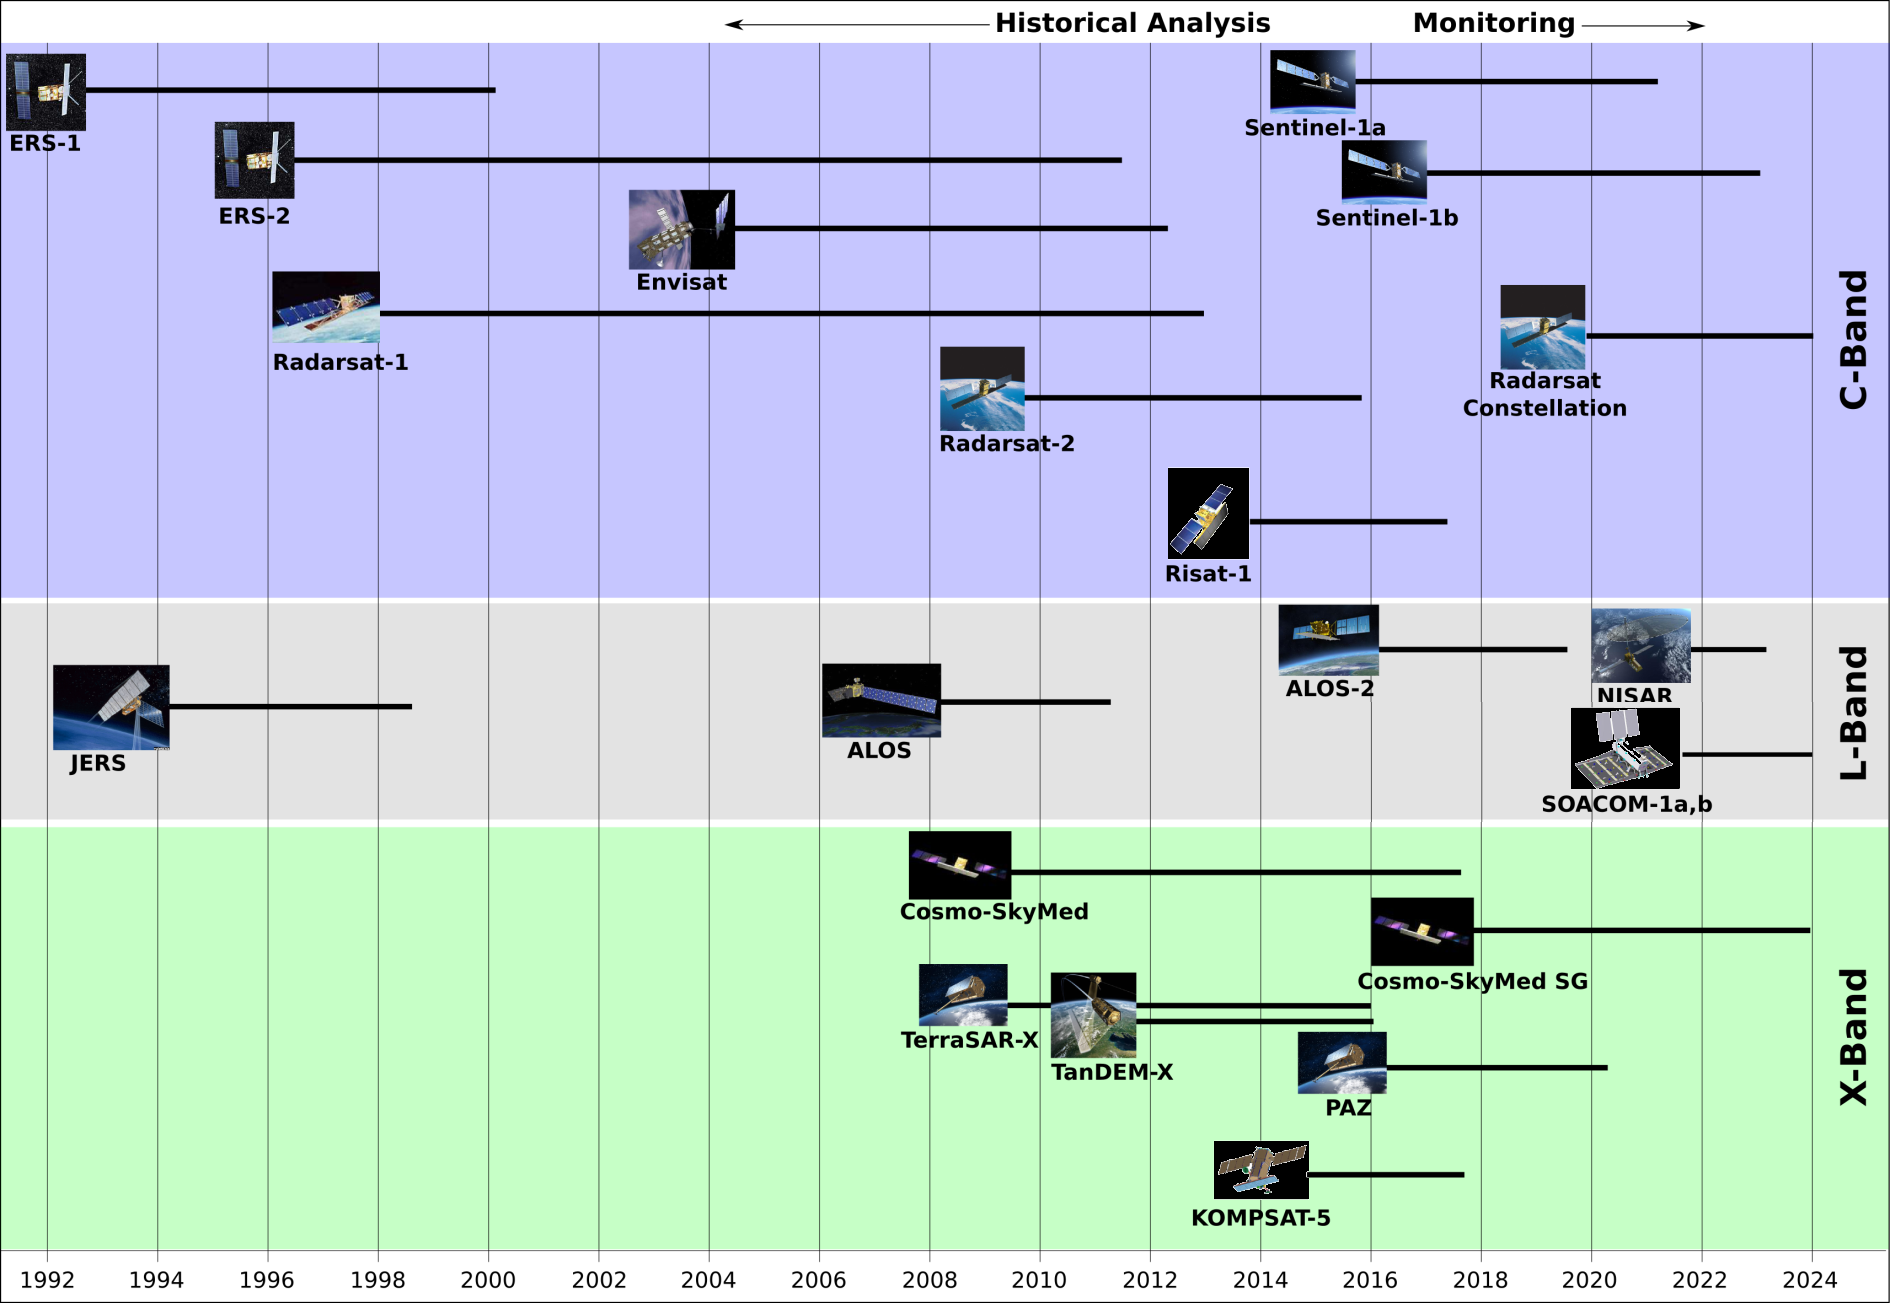
\includegraphics[width=0.7\textwidth]{fig:misiones}
    \caption{Misiones satelitales históricas y actuales.}
    \label{}
  \end{figure}
\end{frame}
%--- Next Frame ---%



\begin{frame}{} \vskip0cm
  \begin{columns}
    \begin{column}{0.6\textwidth}
     \begin{block}{Mision SAOCOM}
\begin{itemize}
  \item Dos satélites idénticos
  \item L-Band SAR (1275 Mhz)
  \item Cobertura Global
  \item Mirada a derecha
  \item Mirada a izquierda
  \begin{itemize}
    \item Hasta 5 minutos
  \end{itemize}
  \item Antena activa de 10m x 3.5m con 140 MTR
\end{itemize}
     \end{block}
    \end{column}
    \begin{column}{0.4\textwidth}  %%<--- here
      \begin{figure}
        \centering
        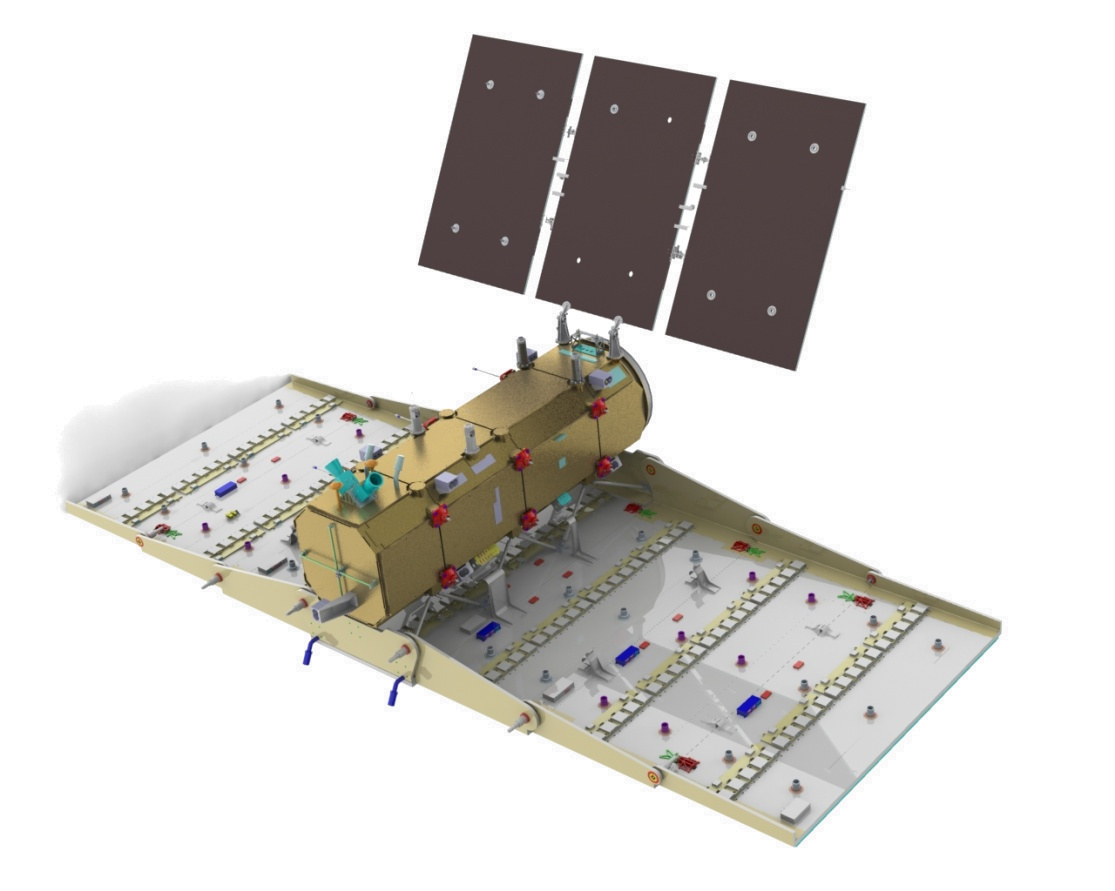
\includegraphics[width=1.1\textwidth]{fig:saocom.jpg}
        \caption*{}
        \label{}
      \end{figure}
    \end{column}
    \end{columns}

\end{frame}
%--- Next Frame ---%

\begin{frame}{} \vskip0cm
  \begin{columns}
    \begin{column}{0.6\textwidth}
     \begin{block}{Mision SAOCOM}
\begin{itemize}
  \item Órbita polar, heliosincrónica (inclinación 97.89) a 620 km de altura.
  \item Cada satélite esta desfasado 180 grados.
  \item Hora local de pasada por el Ecuador en forma ascendente: 6:12 am.
  \item Duración de la orbita 97.2 minutos.
  \item Tiempo de revisita: 16 días (1 satélite)/8 días (constelación)
  \item Órbitas por ciclo: 237.
  \item 23 ciclos por año
\end{itemize}
     \end{block}
    \end{column}
    \begin{column}{0.4\textwidth}  %%<--- here
      \begin{figure}
        \centering
        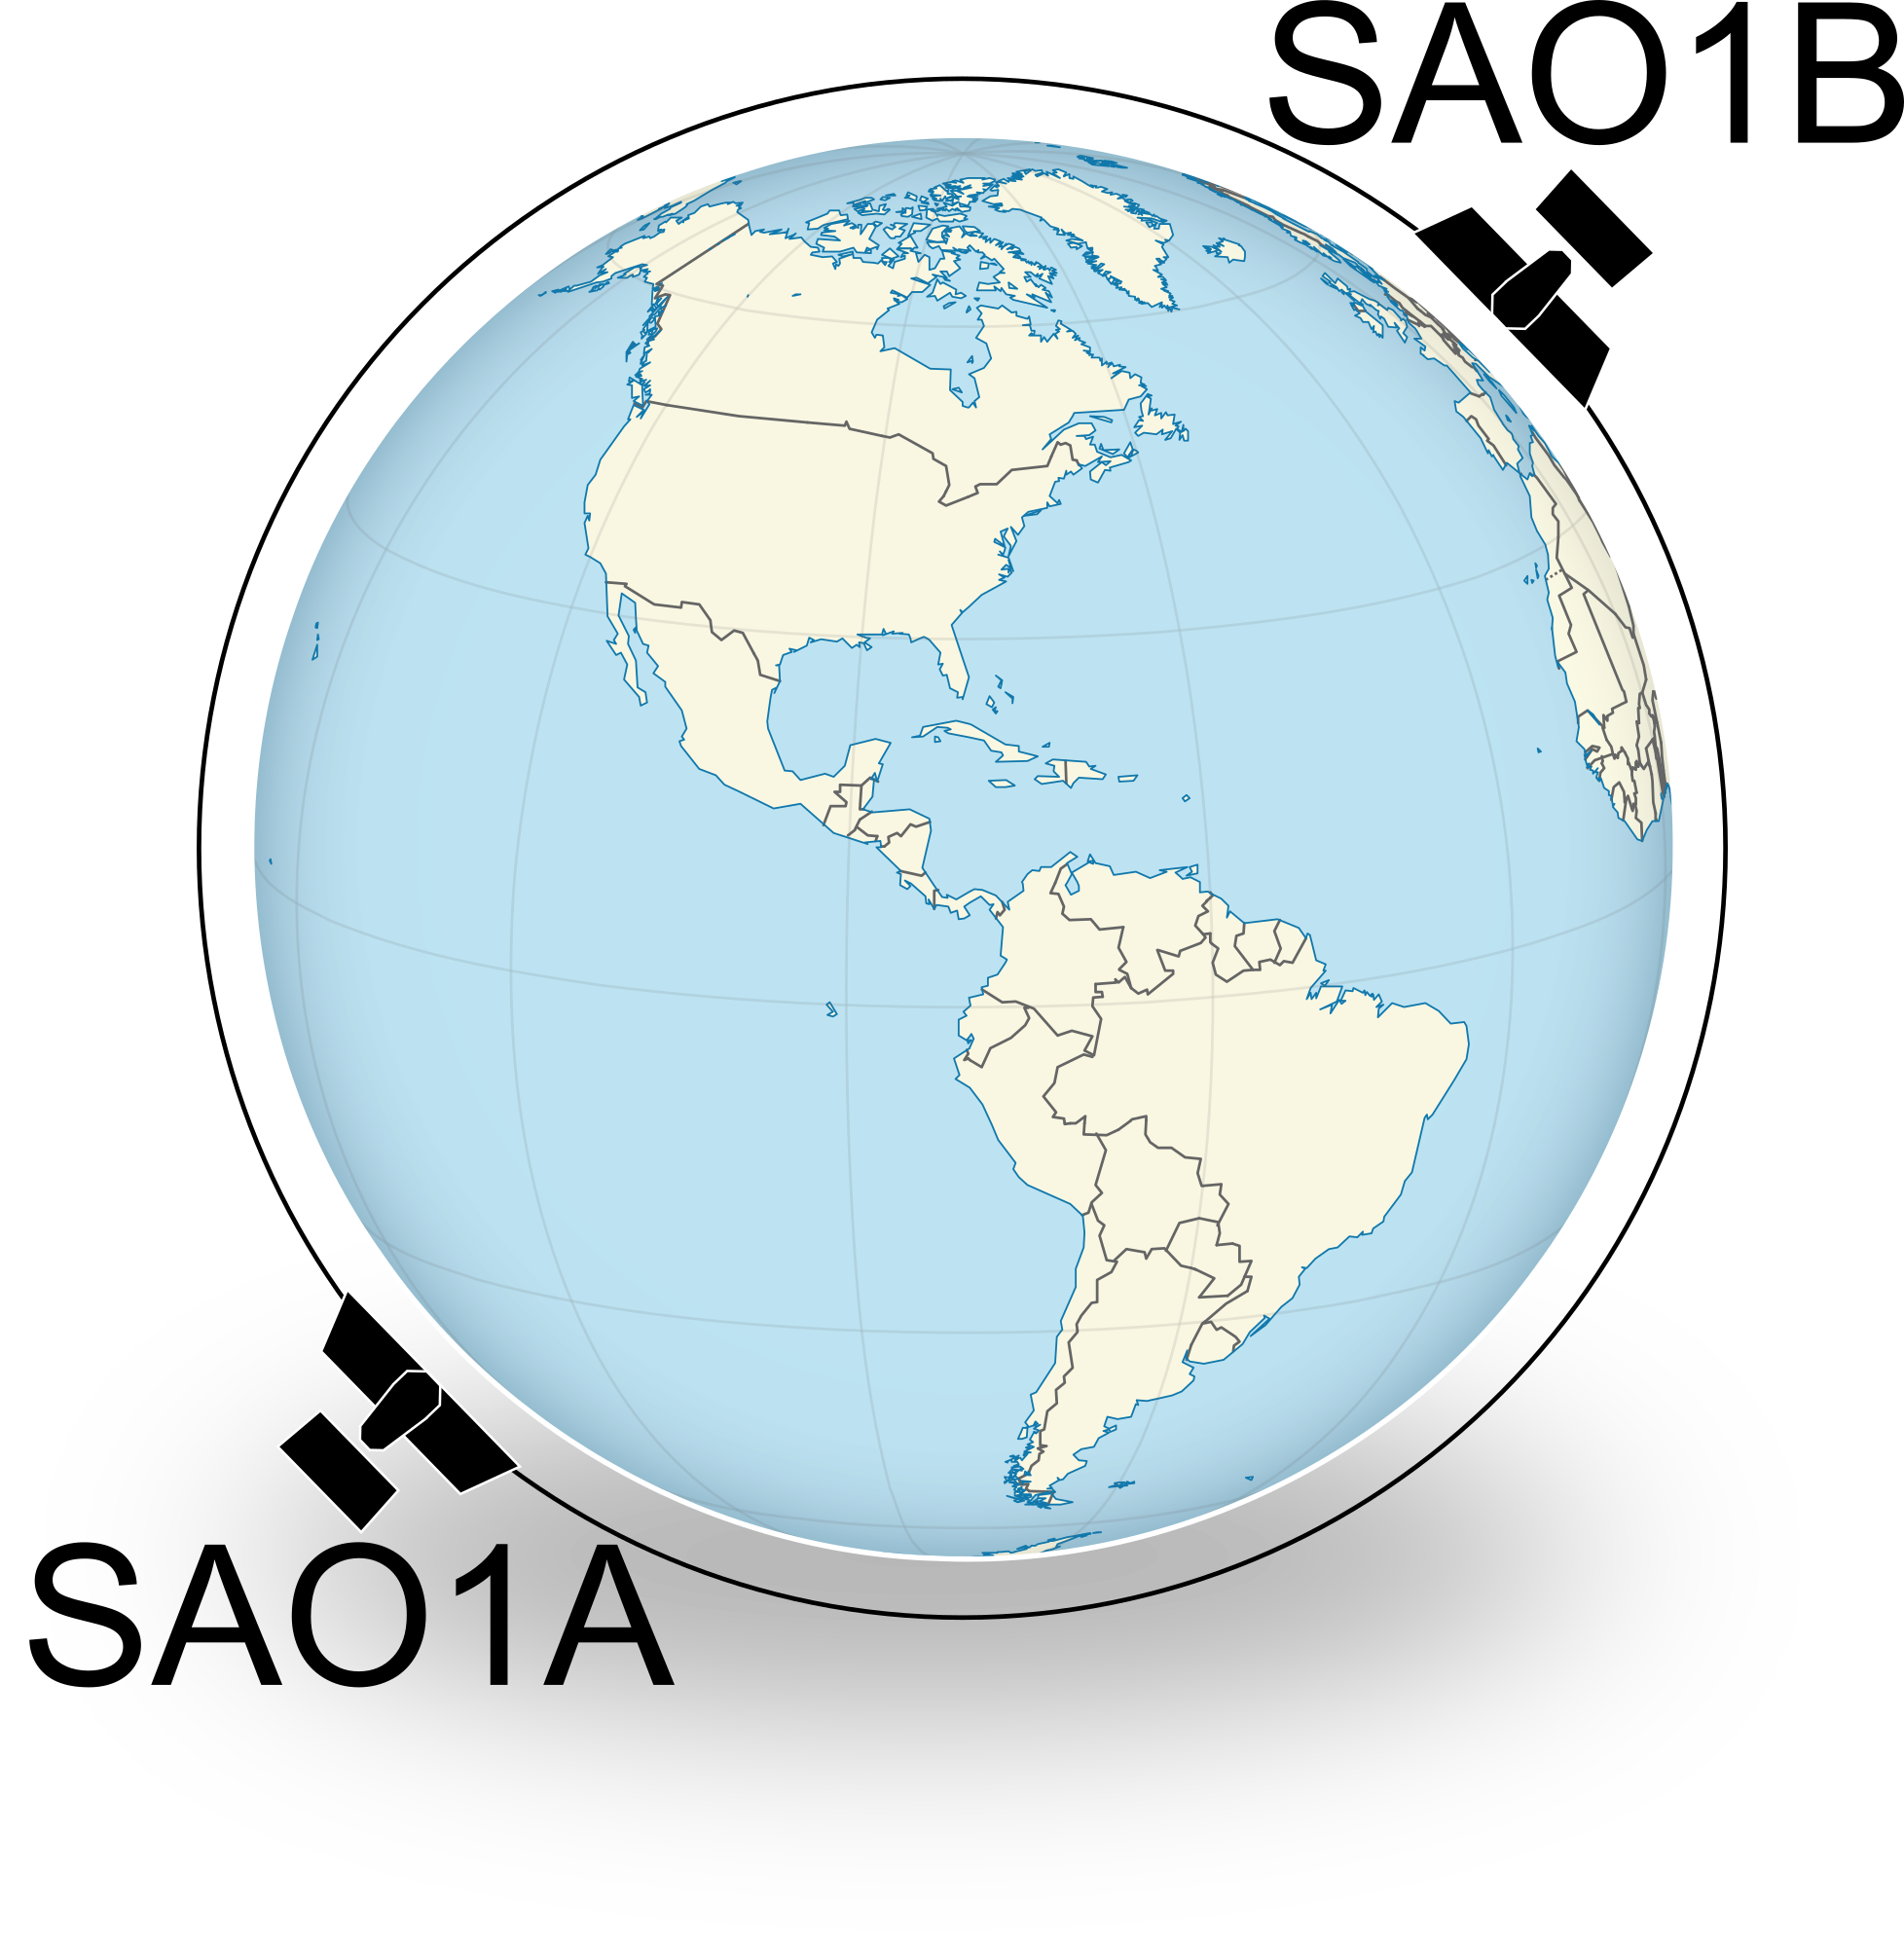
\includegraphics[width=1.1\textwidth]{fig:costelacion.png}
        \caption*{}
        \label{}
      \end{figure}
    \end{column}
    \end{columns}

\end{frame}
%--- Next Frame ---%

\subsection{Aplicaciones SAR}

\begin{frame}{} \vskip0cm
  \begin{figure}
    \centering
    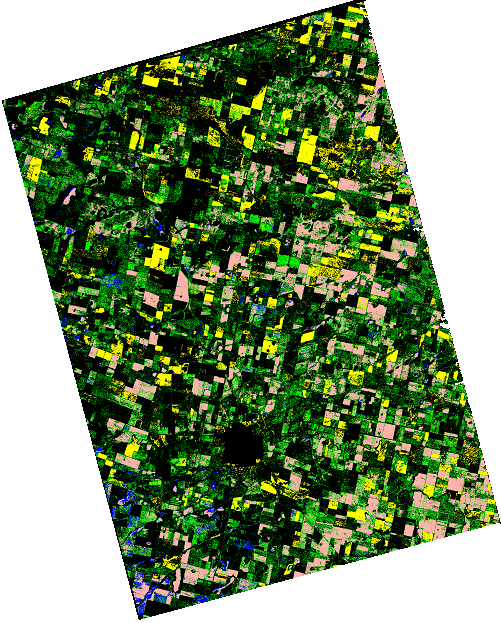
\includegraphics[width=0.35\textwidth]{fig:class.png}
    \caption{Clasificación de cultivos. Rosa: Suelo desnudo, Amarillo: Maiz, Verde: Soja, Agua: Azul, Negro, sin dato. Cosmo SkyMed.}
    \label{}
  \end{figure}
\end{frame}
%--- Next Frame ---%

\begin{frame}{} \vskip0cm
  \begin{figure}
    \centering
    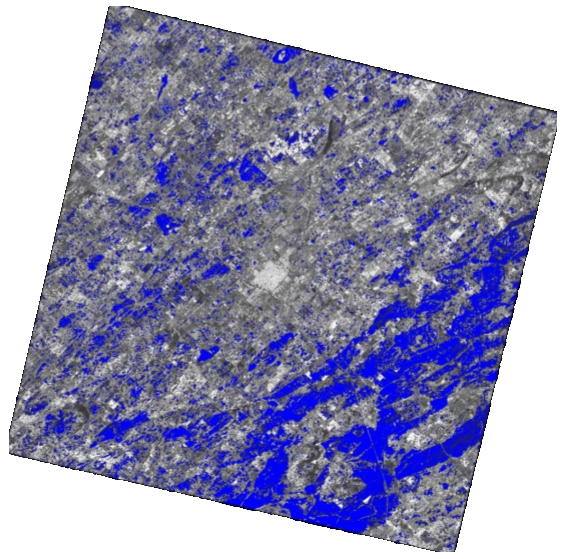
\includegraphics[width=0.48\textwidth]{fig:agua.png}
    \caption{Detección de cuerpos de agua. 19 de agosto de 2017. Cosmo SkyMed.}
    \label{}
  \end{figure}
\end{frame}
%--- Next Frame ---%

\begin{frame}{} \vskip0cm
  \begin{figure}
    \centering
    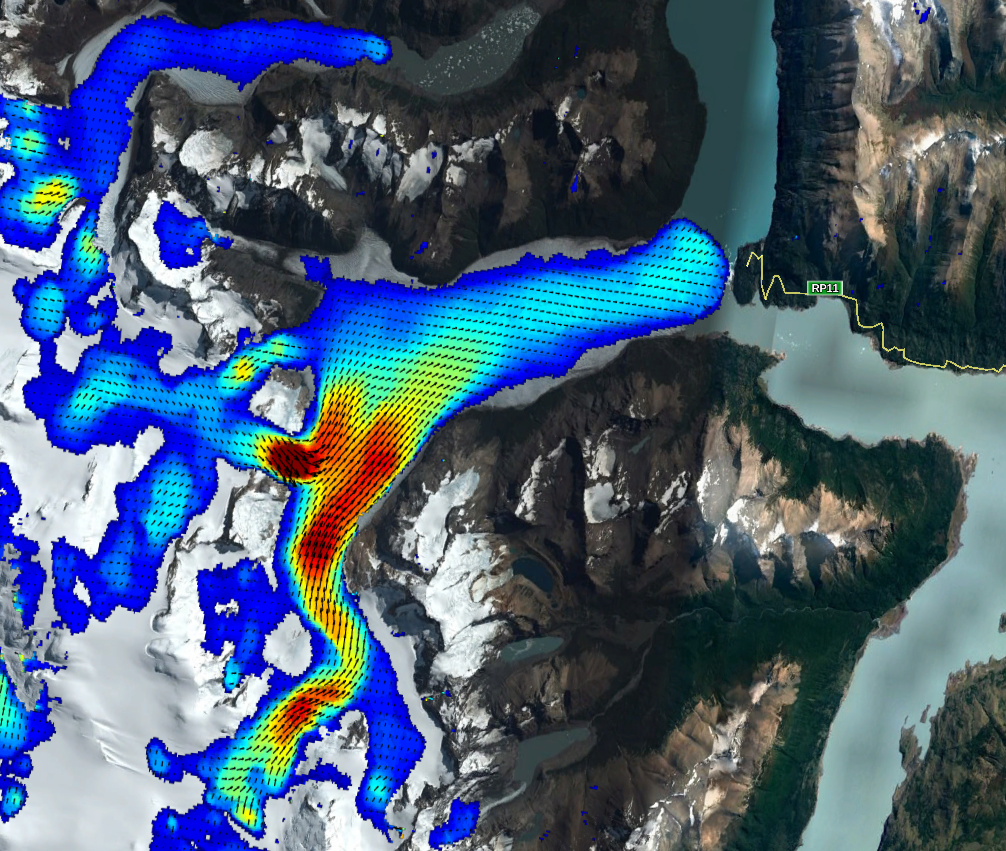
\includegraphics[width=0.5\textwidth]{fig:glaciar.png}
    \caption{Velocidad de desplazamiento de glaciares. Glaciar Perito Moreno. COSMO-SkyMed.}
    \label{}
  \end{figure}
\end{frame}
%--- Next Frame ---%

\begin{frame}{} \vskip0cm
  \begin{figure}
    \centering
    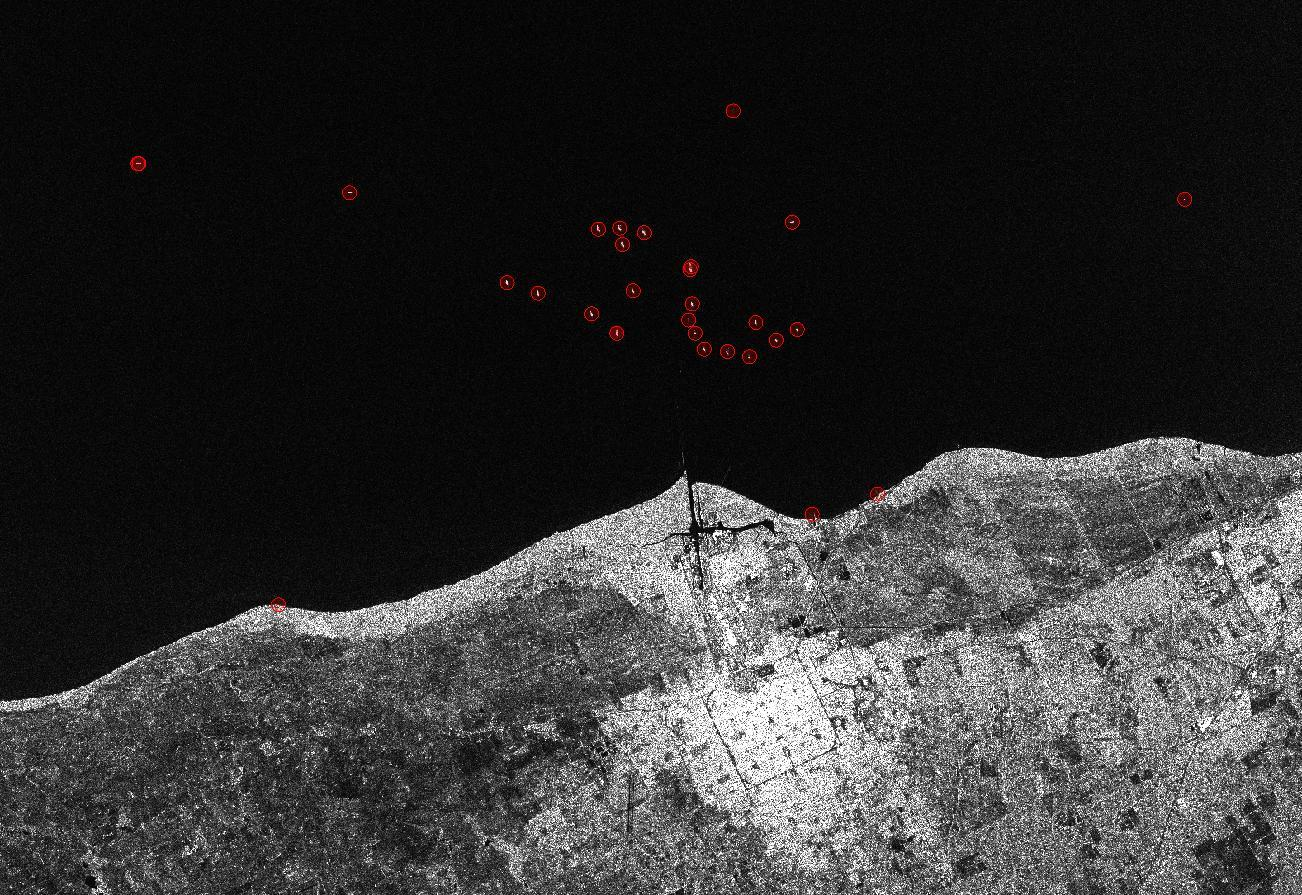
\includegraphics[width=0.6\textwidth]{fig:barcos.jpg}
    \caption{Detección de barcos frente a la ciudad de La Plata. 6 de diciembre de 2017. Sentinel 1.}
    \label{}
  \end{figure}
\end{frame}
%--- Next Frame ---%

\begin{frame}{} \vskip0cm
  \begin{figure}
    \centering
    \includegraphics[width=0.6\textwidth]{fig:expansion.png}
    \caption{Detección de áreas urbanas. Ciudad de La Plata y alrededores.}
    \label{}
  \end{figure}
\end{frame}
%--- Next Frame ---%

\begin{frame}{} \vskip0cm
  \begin{figure}
    \centering
    \includegraphics[width=0.65\textwidth]{fig:volcan.png}
    \caption{Deformación de la superficie por erupción del Volcán Calbuco, 22 de abril de 2015. Imagen ALOS PALSAR 2.}
    \label{}
  \end{figure}
\end{frame}
%--- Next Frame ---%

\begin{frame}{} \vskip0cm
  \begin{figure}
    \centering
    \includegraphics[width=0.75\textwidth]{fig:subduccion.jpg}
    \caption{Detección de subsidencia por métodos interferométricos.}
    \label{}
  \end{figure}
\end{frame}
%--- Next Frame ---%

\begin{frame}{} \vskip0cm
  \begin{figure}
    \centering
    \includegraphics[width=0.65\textwidth]{fig:dem.png}
    \caption{Modelo digital de elevación (DEM). Cosmo SkyMed.}
    \label{}
  \end{figure}
\end{frame}
%--- Next Frame ---%


\gracias
%--- Next Frame ---%


\end{document}
